% Created 2023-01-09 Mon 11:54
% Intended LaTeX compiler: pdflatex
\documentclass{wx672ctexart} \usepackage{hyperref}
\usepackage{amsmath,amsfonts,amssymb}
\usepackage{graphicx}
\usepackage{tabularray}
\usepackage{minted}
\author{王晓林}
\date{\today}
\title{Debian快速安装指导}
\hypersetup{
 pdfauthor={王晓林},
 pdftitle={Debian快速安装指导},
 pdfkeywords={},
 pdfsubject={},
 pdfcreator={Emacs 28.2 (Org mode 9.5.5)}, 
 pdflang={Cn}}
\begin{document}

\maketitle
\tableofcontents


\section{UEFI}
\label{sec:org2d26eb1}
现在(2018年10月)的电脑都很新潮,在主板上几乎都用UEFI取代了传统的BIOS。关于UEFI设置,我的
经验是:

\begin{itemize}
\item 把下列和Windows相关的选项都关掉(disable):
\begin{itemize}
\item \texttt{Secure boot}
\item \texttt{QuickBoot/FastBoot}
\item \texttt{Intel Smart Response Technology (SRT)}
\item \texttt{FastStartup}
\end{itemize}

\item 如果在下面的安装过程中(硬盘分区的时候)看不到硬盘,那么你需要在UEFI设置里找到Intel Rapid Storage
Technology (Intel RST),把它设置为AHCI。
\end{itemize}

\section{安装最小系统}
\label{sec:org94724dc}

【注意事项】为了避免不必要的麻烦:

\begin{enumerate}
\item 不要选择图形界面安装(Graphical Install); \textbf{不要图形界面}; \textbf{不要图形界面};
\item 不要选择中文安装界面; \textbf{不要中文}; \textbf{不要中文};
\item 不要为root设置密码; \textbf{不要root密码}; \textbf{不要root密码};
\item 安装过程中不要联网; \textbf{不要联网}; \textbf{不要联网};
\item 只要两个分区 \texttt{swap} 和 \texttt{/} ,换言之,不要 \texttt{/boot, /home, /var, ...} 等分区。
\end{enumerate}

安装Debian最小系统的大致步骤如下:

\begin{enumerate}
\item 先准备好一个安装盘(LiveUSB)
\begin{enumerate}
\item \textbf{下载:} \url{https://cdimage.debian.org/cdimage/unofficial/non-free/cd-including-firmware/current/amd64/iso-cd/}
\begin{itemize}
\item 该目录中有两个(也许更多)iso文件,下载名字最短的那个就好。比如:
\begin{verbatim}
firmware-11.6.0-amd64-netinst.iso     <-- 只要这个
firmware-edu-11.6.0-amd64-netinst.iso        
\end{verbatim}
\end{itemize}

\item \textbf{制作U盘:} 在Debian/Ubuntu平台上制作启动U盘非常简单,敲个命令就行了:
\begin{minted}[mathescape=true,linenos=true,numbersep=5pt,frame=lines,framesep=2mm]{sh}
sudo cp fir<TAB> /dev/sdX  # <TAB> 指的是键盘上的 TAB 键,它能帮你补全文件名。
						   # 把 sdX 换成 sdb 或者 sdc。用 lsblk 命令看一眼,
						   # 就知道是 b 还是 c 了。
sync
\end{minted}
【注意】
\begin{itemize}
\item \textbf{如果没有现成的Linux系统,只有Windows可用,怎么做启动U盘?} 抱歉,我也不知道。我
知道肯定可以,而且见人做过,只不过我真的不用Windows,所以真的不关心。
\end{itemize}
\end{enumerate}
\item 拔掉网线,从U盘重启系统,开始安装。大概半个小时,一个“最小系统”就装
好了。「拔掉网线」只是我的个人习惯,并不是必须的。联网安装的话,可能会遭遇若干问题:
\begin{enumerate}
\item 如果网络不畅,安装过程会很慢,甚至失败;
\item 现在时髦的笔记本都不带有线网口,如果选择联网安装,安装过程中就要涉及安装网卡驱动、输
入无线密码等步骤,麻烦多多;
\item 联网安装,系统还会提示你选择镜像源、选择要安装的“全家桶”,这些貌似友好的功能选项,在
我看弊大于利,只能增加入门者的困扰。
\end{enumerate}
\item 完事后,拔掉U盘,重启系统。
\item 【注意】
\begin{itemize}
\item 安装的时候 \textbf{不要选择中文语言环境}, 因为后面的安装配置工作都是在非图形环境下进行,
采用中文的话,你很可能会遭遇乱码。
\item 提示你“Loading missing firmware”的时候,选择“NO”。
\item “Configure the network”的时候,选择一连串的“Cancel”,直到你看到“Do not configure the
network at this time”。
\item 看到提示“Root password:”的时候,不要给密码,直接回车跳过这一步。
\item 看到“continue without a network mirror?”的时候,选择 <Yes>。
\item 硬盘分区的时候,如果你是装Linux单系统,就非常简单,没啥可说的;如果你是要装双系统(保
留原来的Windows),那么,有三点烦,
\begin{enumerate}
\item 可用空间不够怎么办?删掉哪个分区?如何压缩原来的Windows分区?总之,烦!
\item 以后,霸道的Windows每次升级、更新,都会让你的Linux消失……
\item 装了双系统之后,通常(不争气的)你会选用熟悉的Windows系统,渐渐地,过不了多久,你就忘了电
脑上还有一个Linux系统。
\end{enumerate}
所以,我很不愿意搭理装双系统的人。
\end{itemize}
\end{enumerate}
\subsection{截图}
\label{sec:orgc37e52e}

\begin{enumerate}
\item 开始安装,选择“Install”,不要选“Graphical install”

\begin{center}
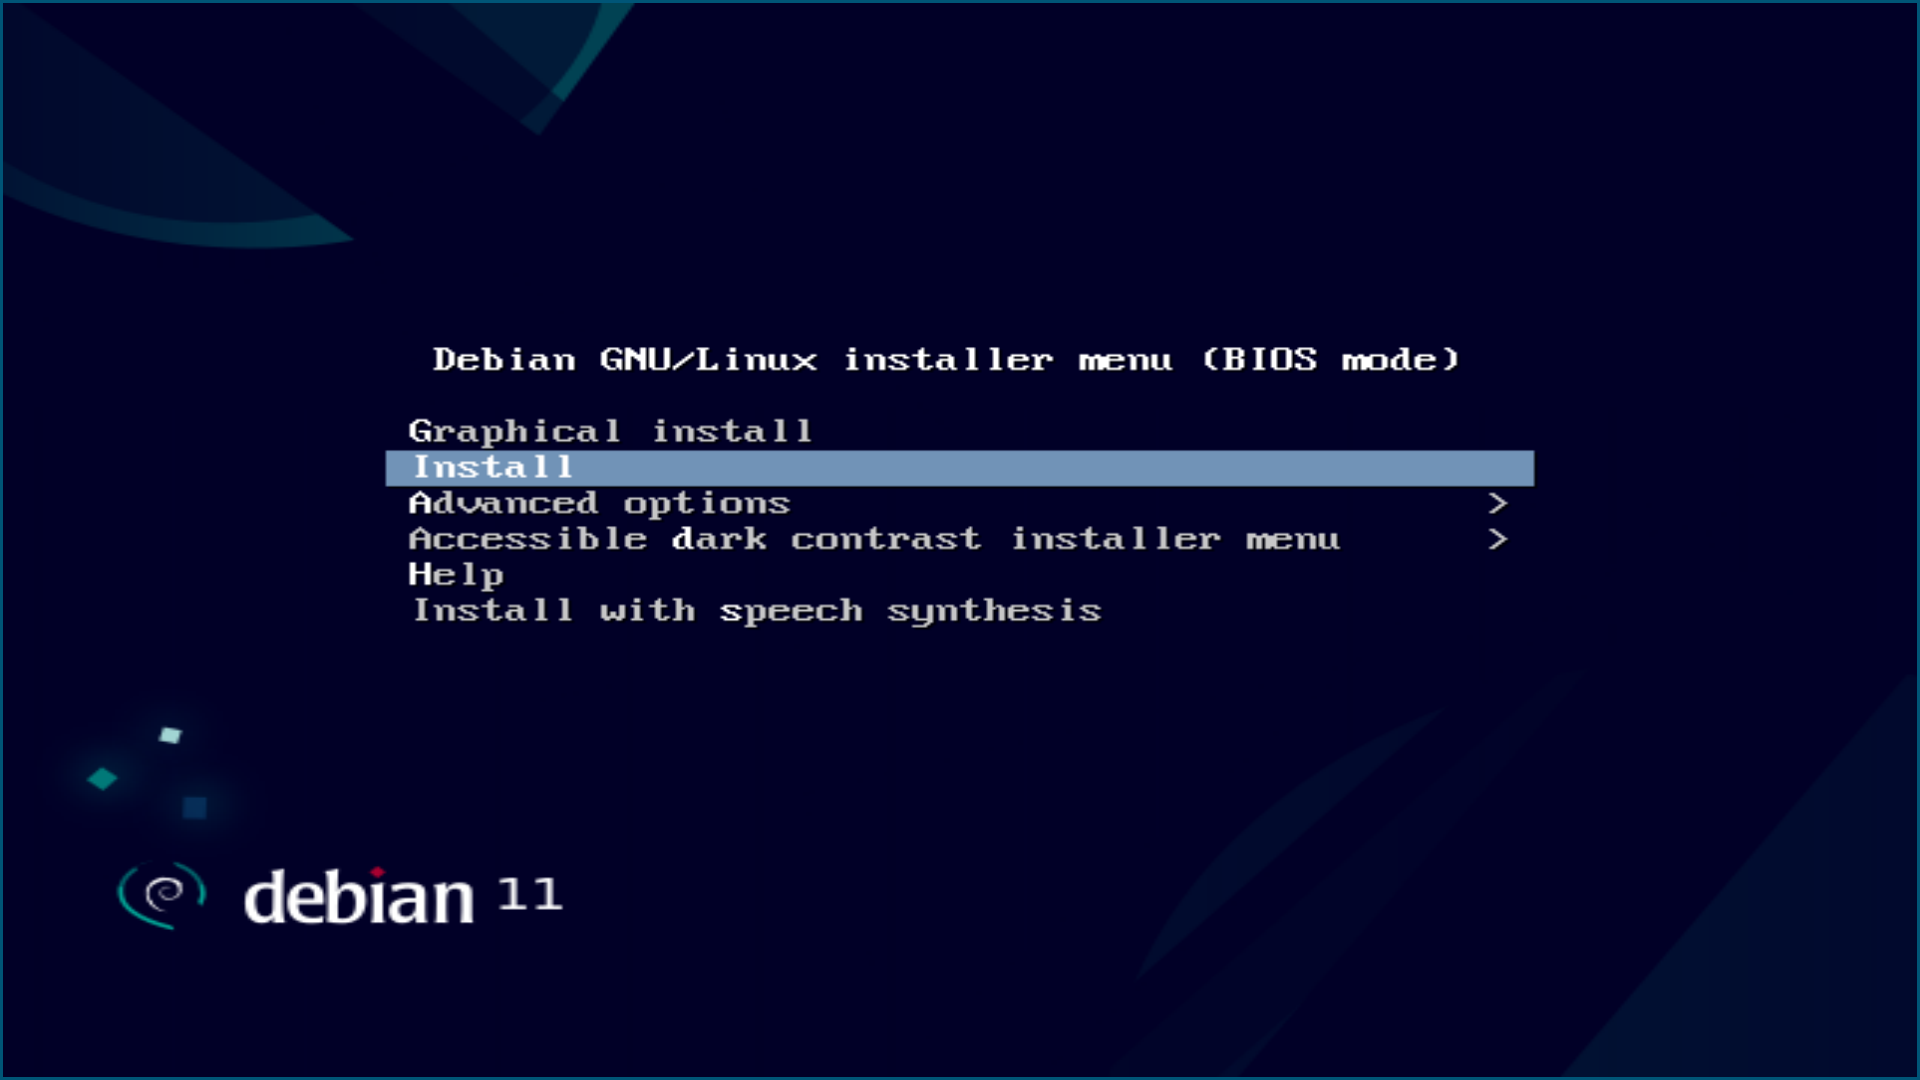
\includegraphics[width=.5\linewidth]{screenshots/01.png}
\end{center}

\item 选择“English”,千万别选“中文”!

\begin{center}
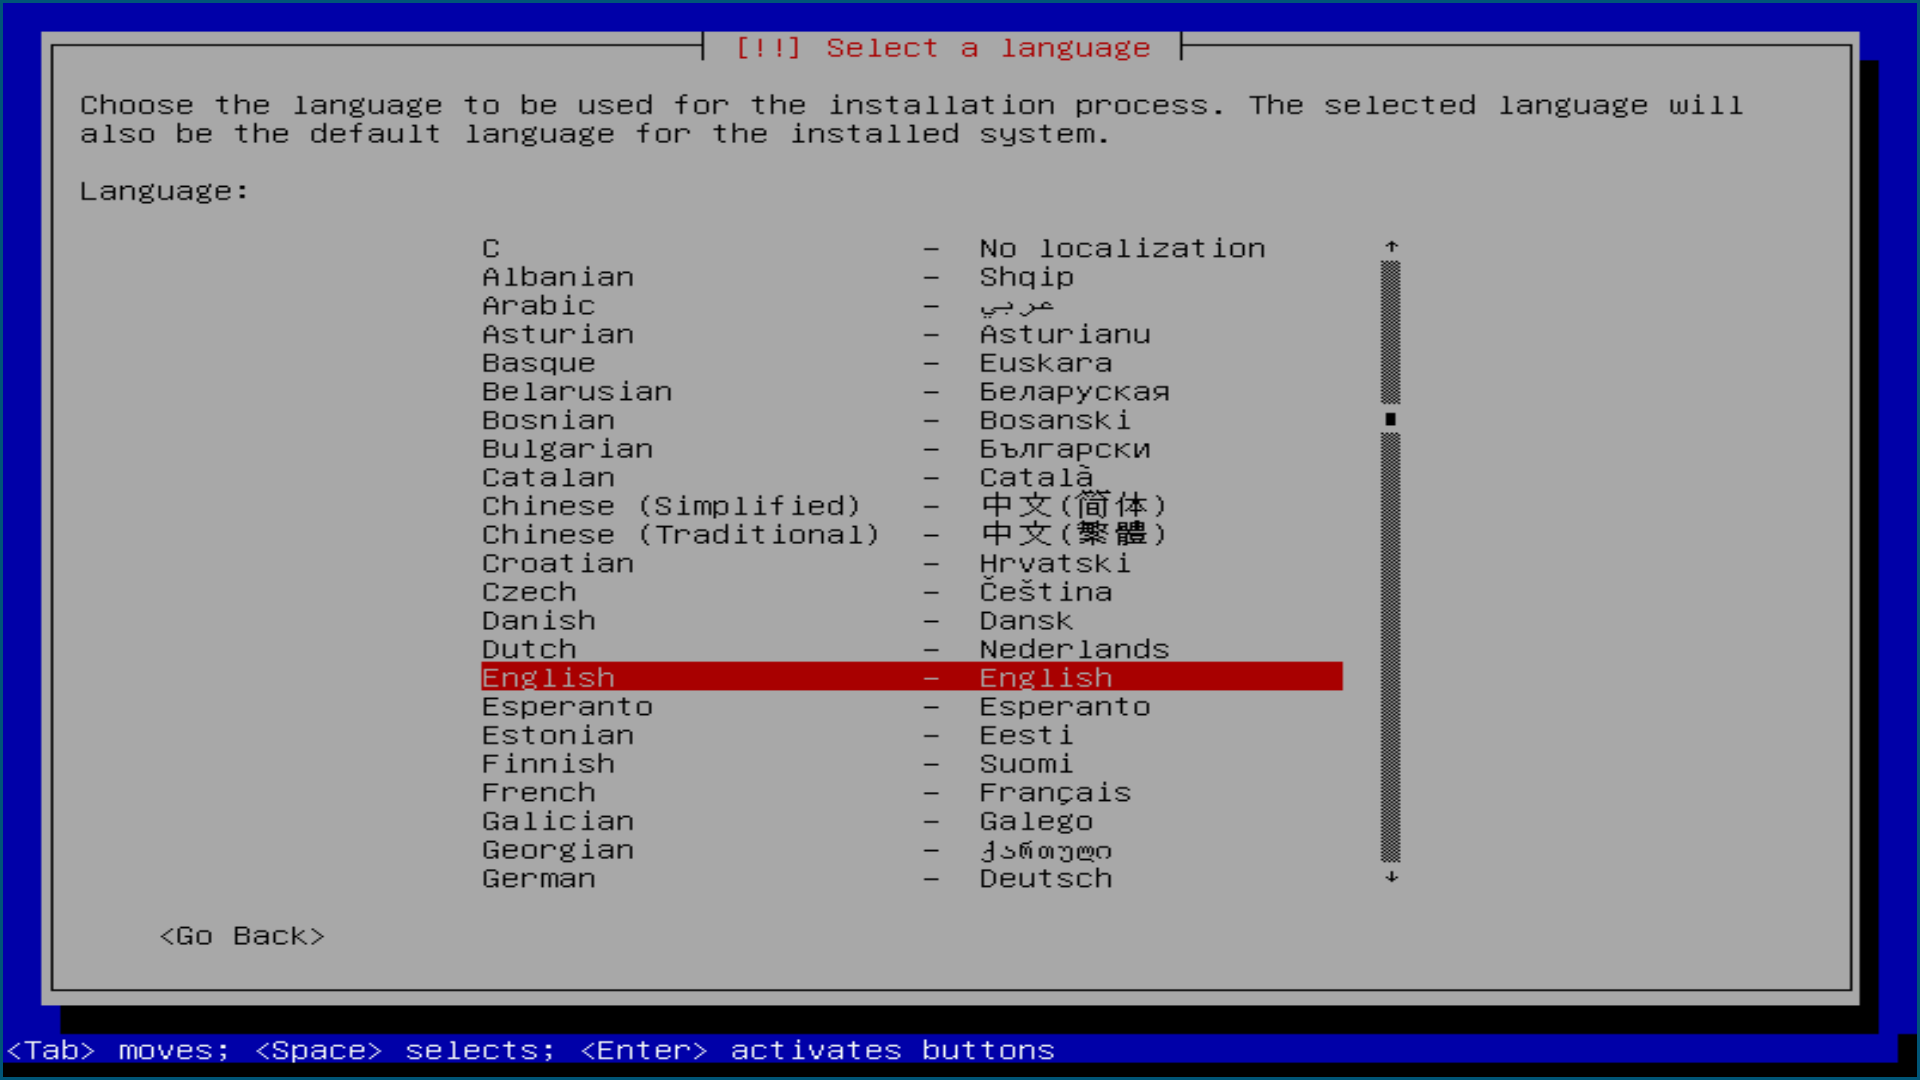
\includegraphics[width=.5\linewidth]{screenshots/02.png}
\end{center}

\item 这一步不重要,回车接受默认值就好

\begin{center}
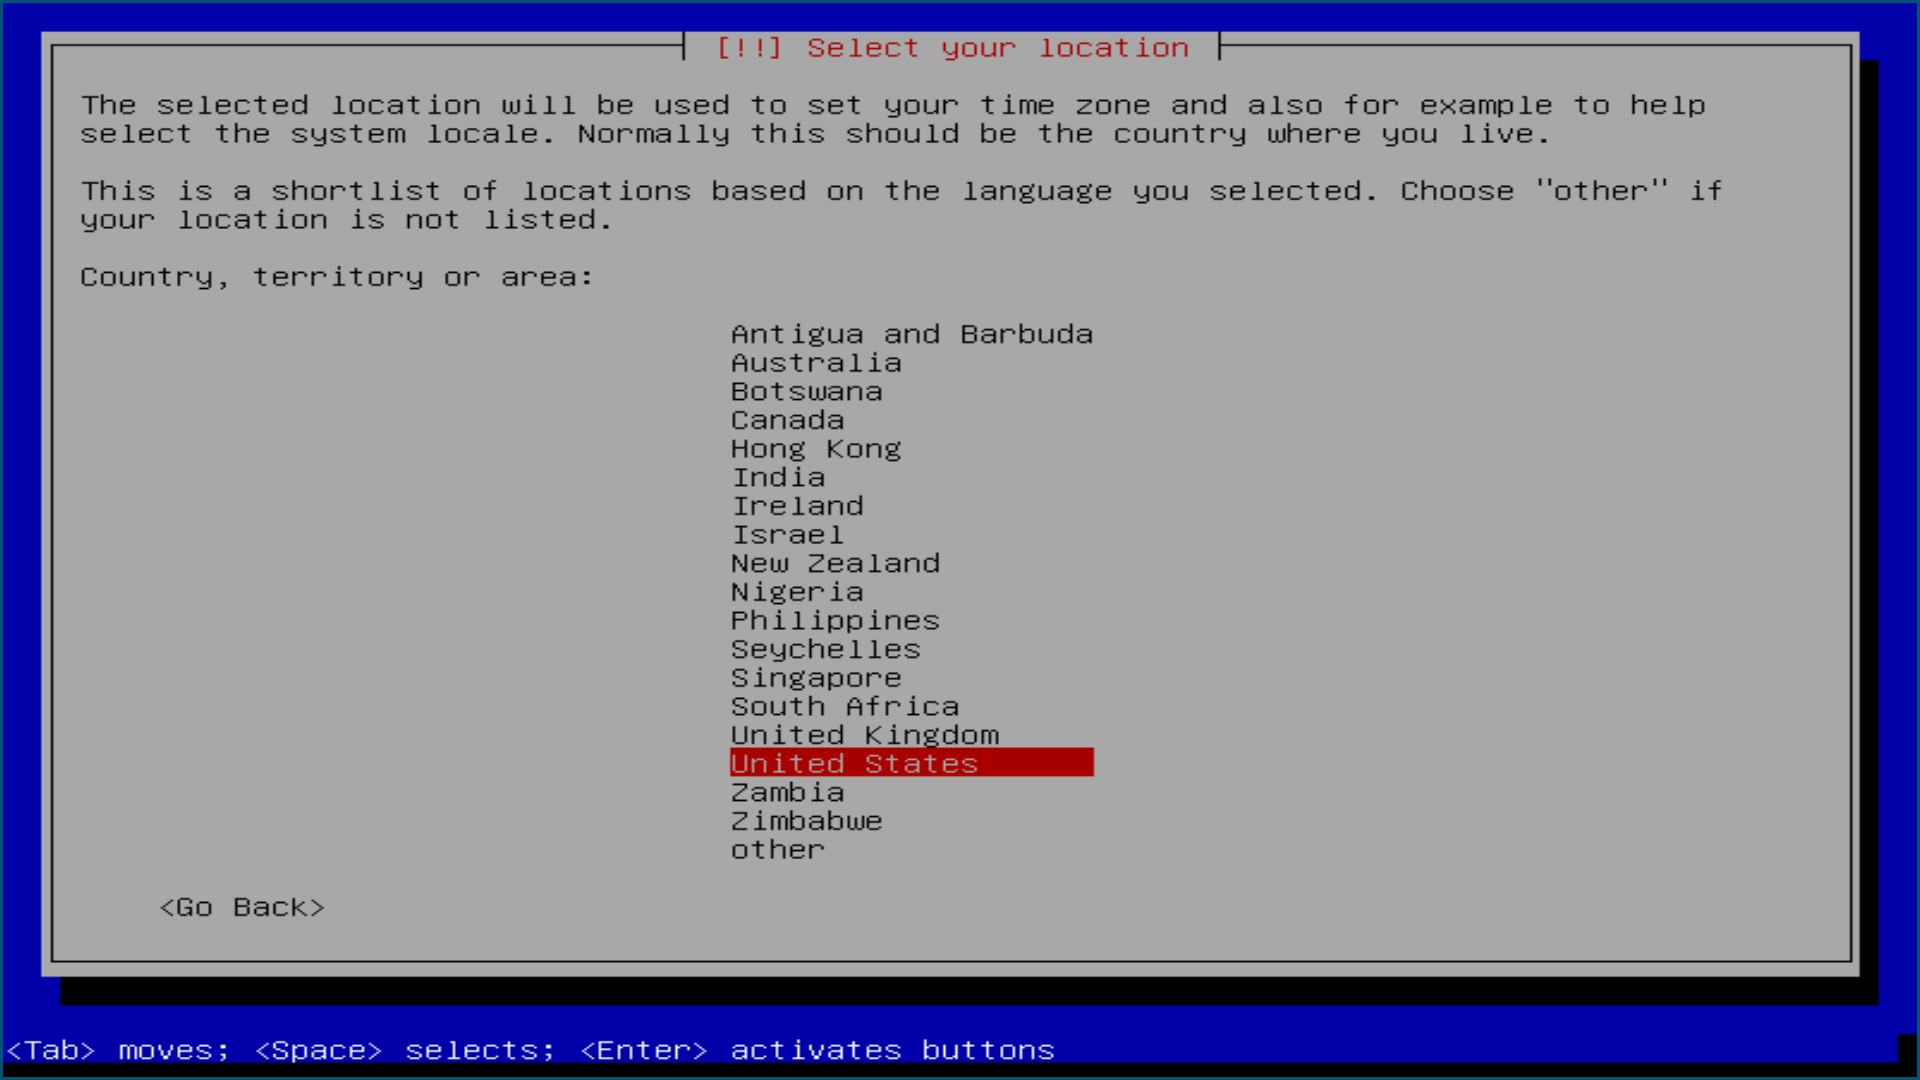
\includegraphics[width=.5\linewidth]{screenshots/03.png}
\end{center}

\item 回车接受默认值

\begin{center}
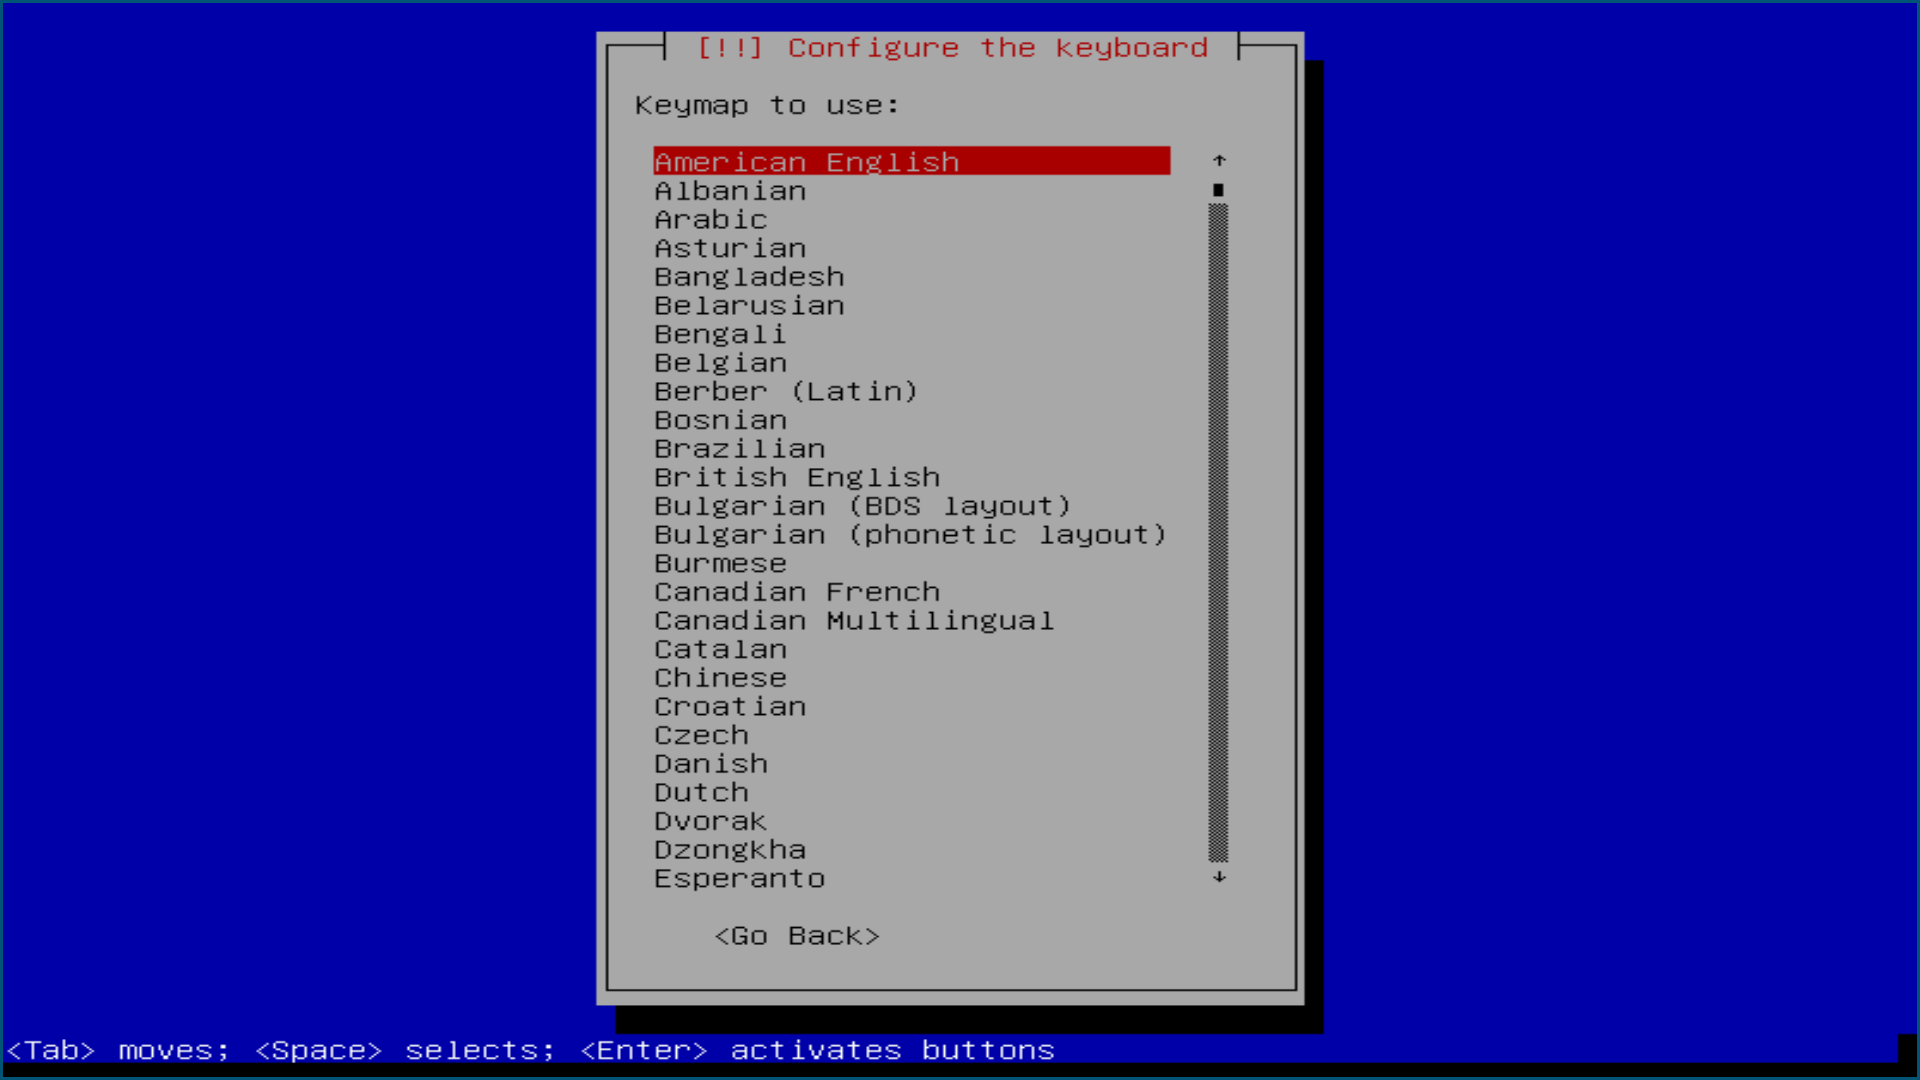
\includegraphics[width=.5\linewidth]{screenshots/04.png}
\end{center}

\item 配置网络的时候手要快,见到“Cancel”就按,打断配置,因为我们暂时不需要联网。

\begin{center}
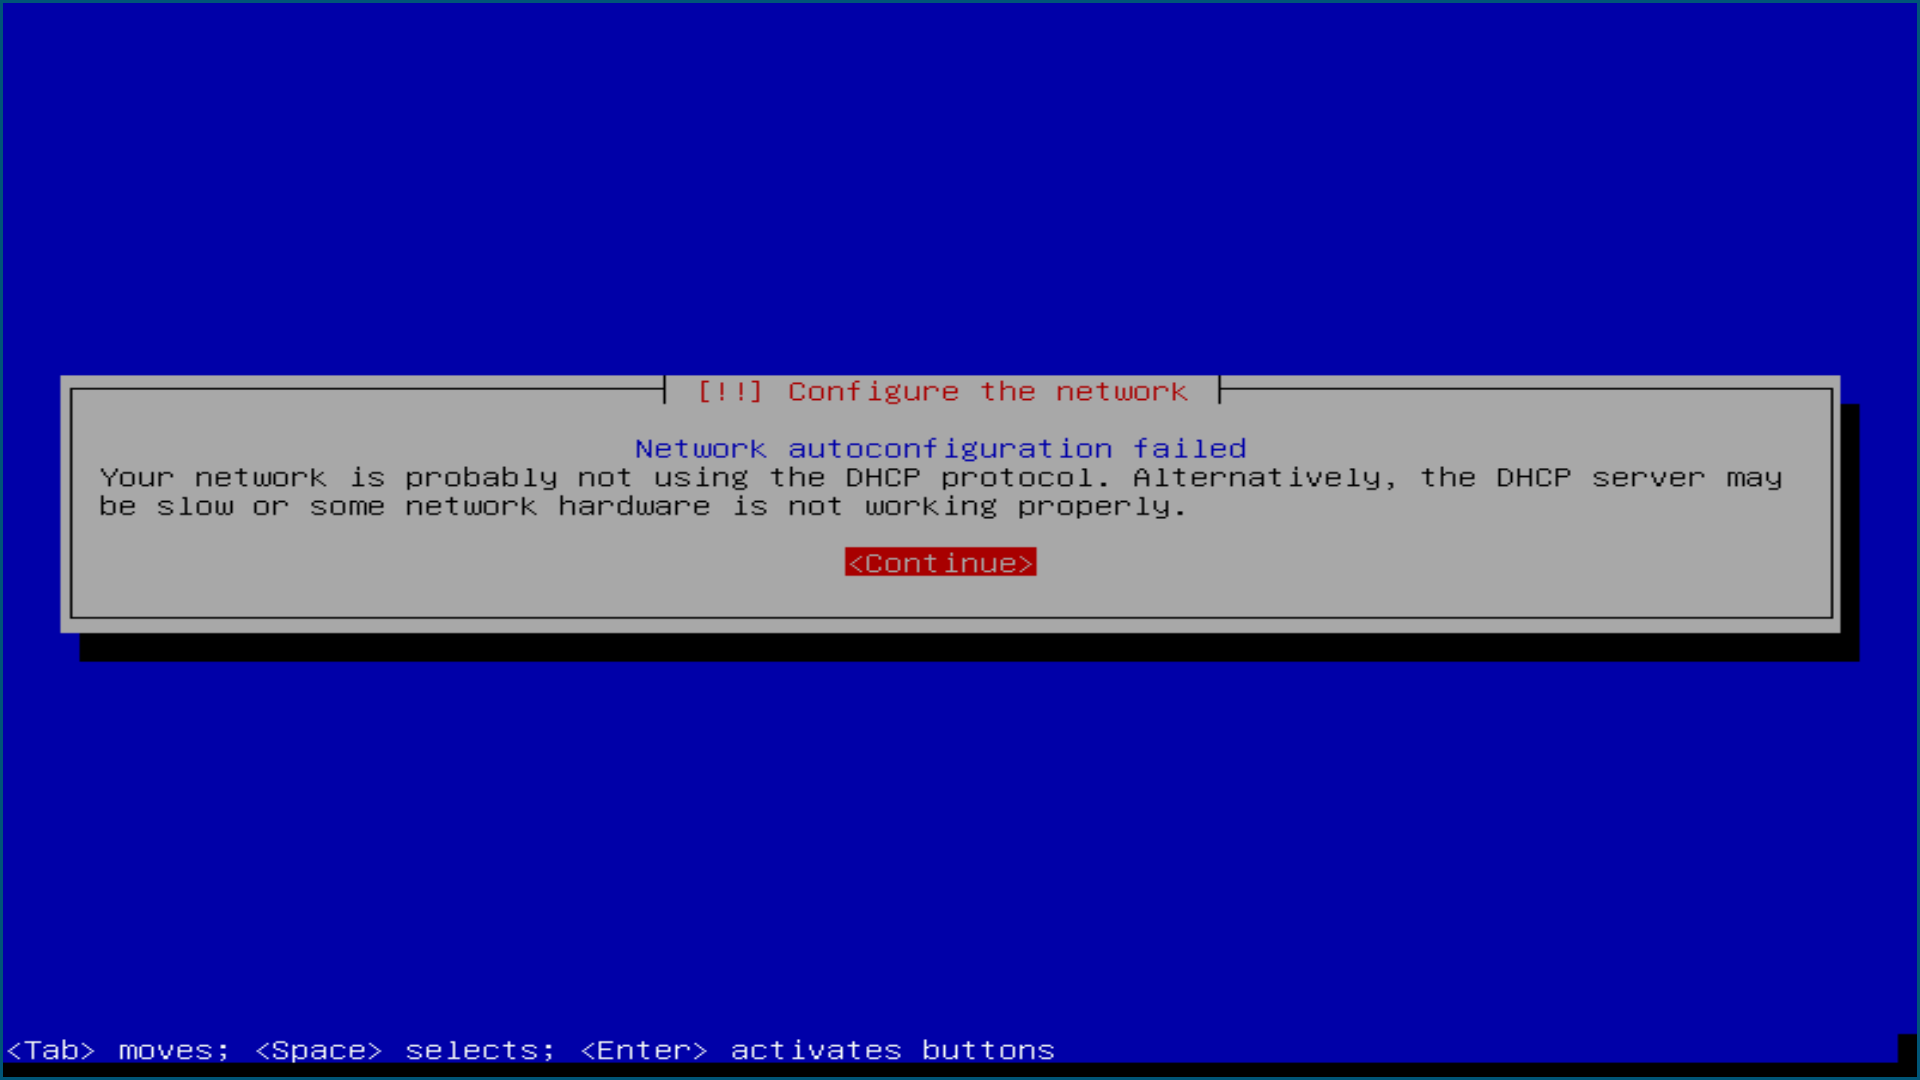
\includegraphics[width=.5\linewidth]{screenshots/05.png}
\end{center}

\begin{figure}[htbp]
\centering
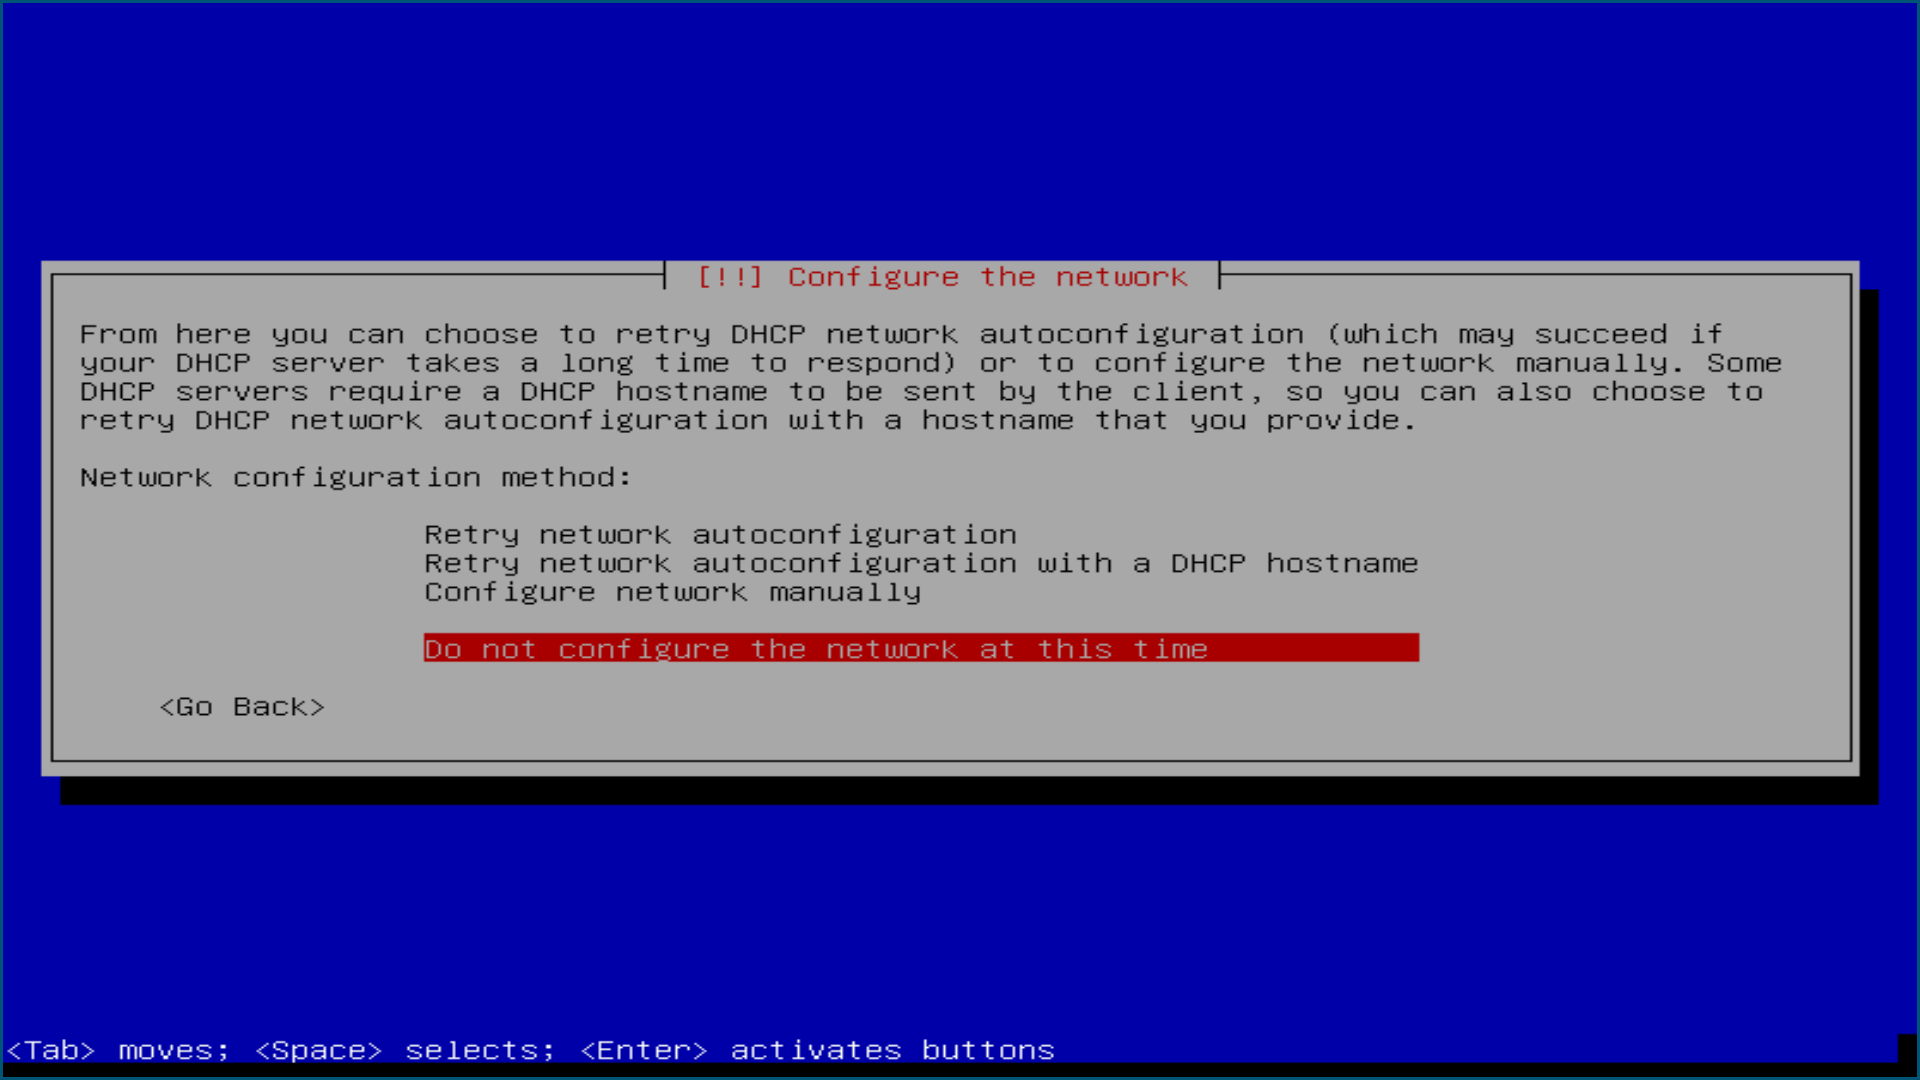
\includegraphics[width=.5\linewidth]{screenshots/06.png}
\caption{一定要选“Do not configure the network at this time”}
\end{figure}

\item 回车接受默认值

\begin{center}
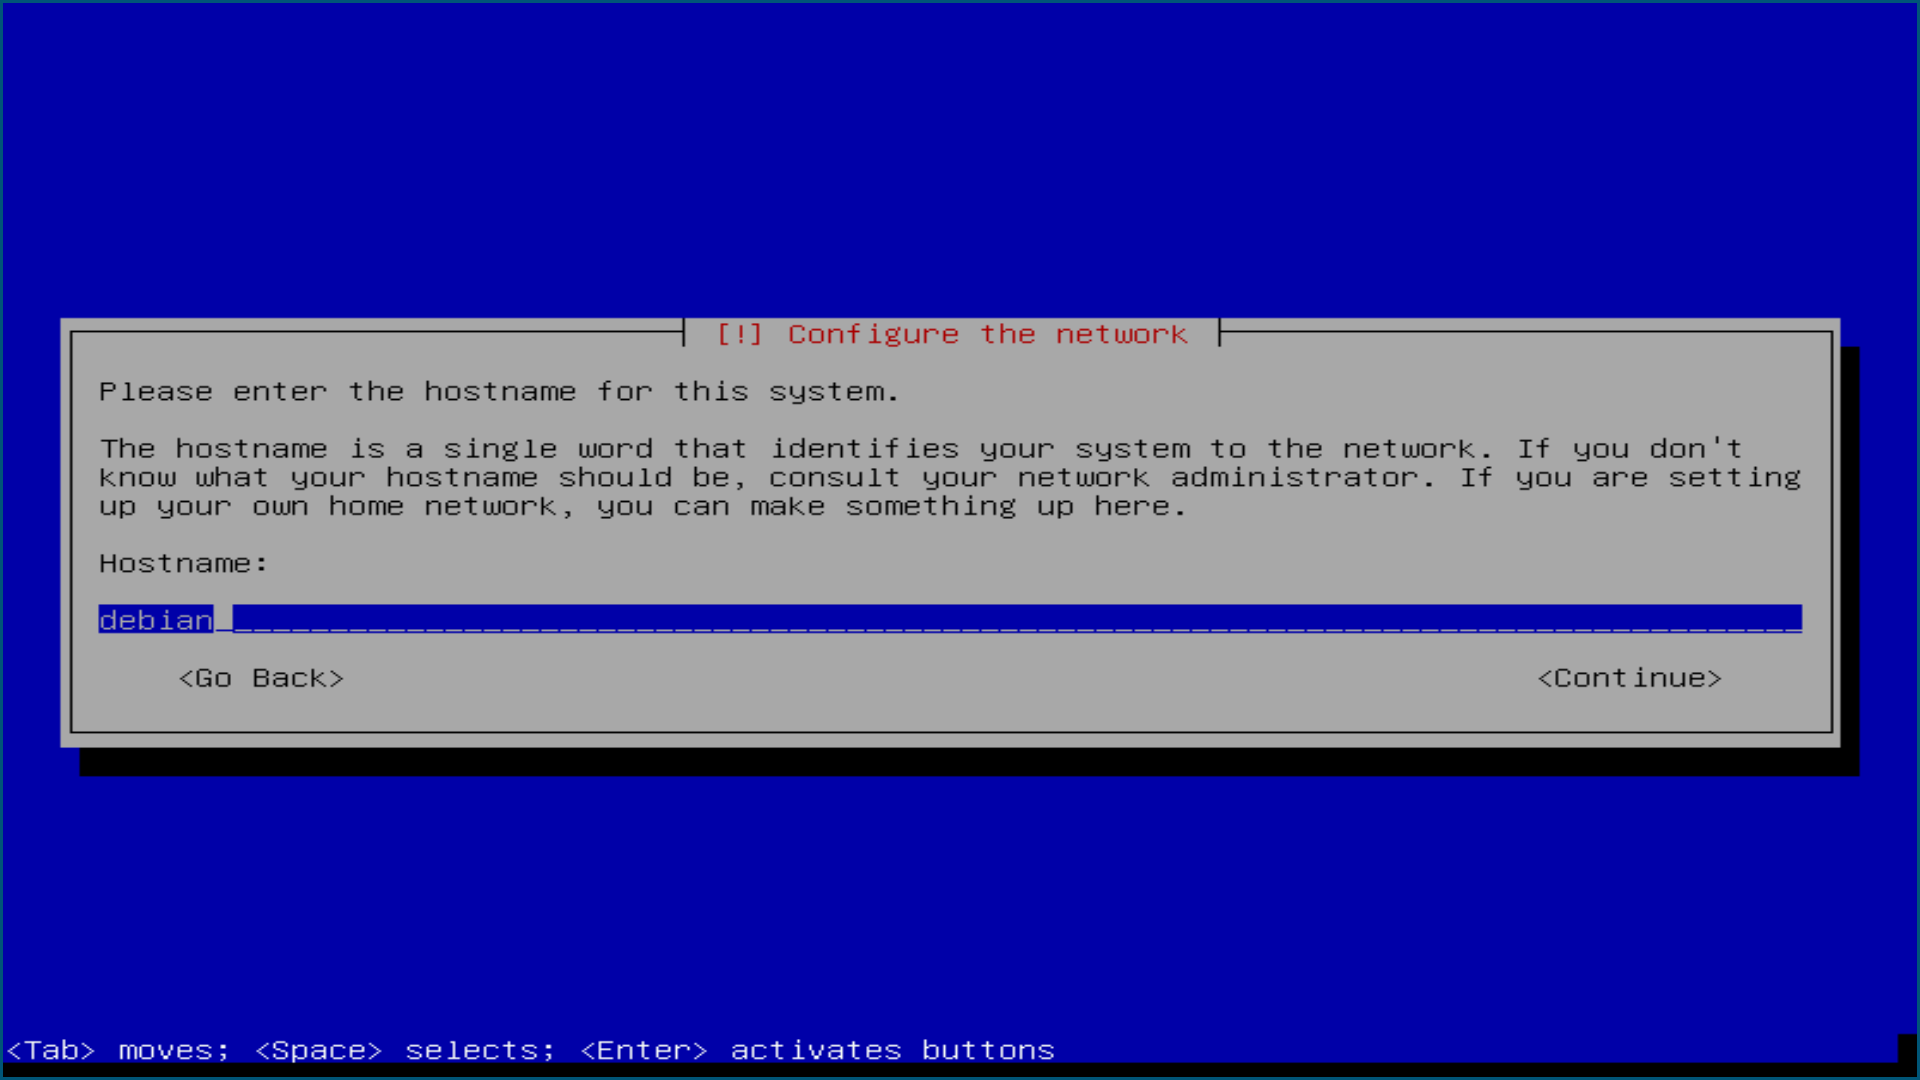
\includegraphics[width=.5\linewidth]{screenshots/07.png}
\end{center}

\item 回车跳过,不要给root设置密码!

\begin{center}
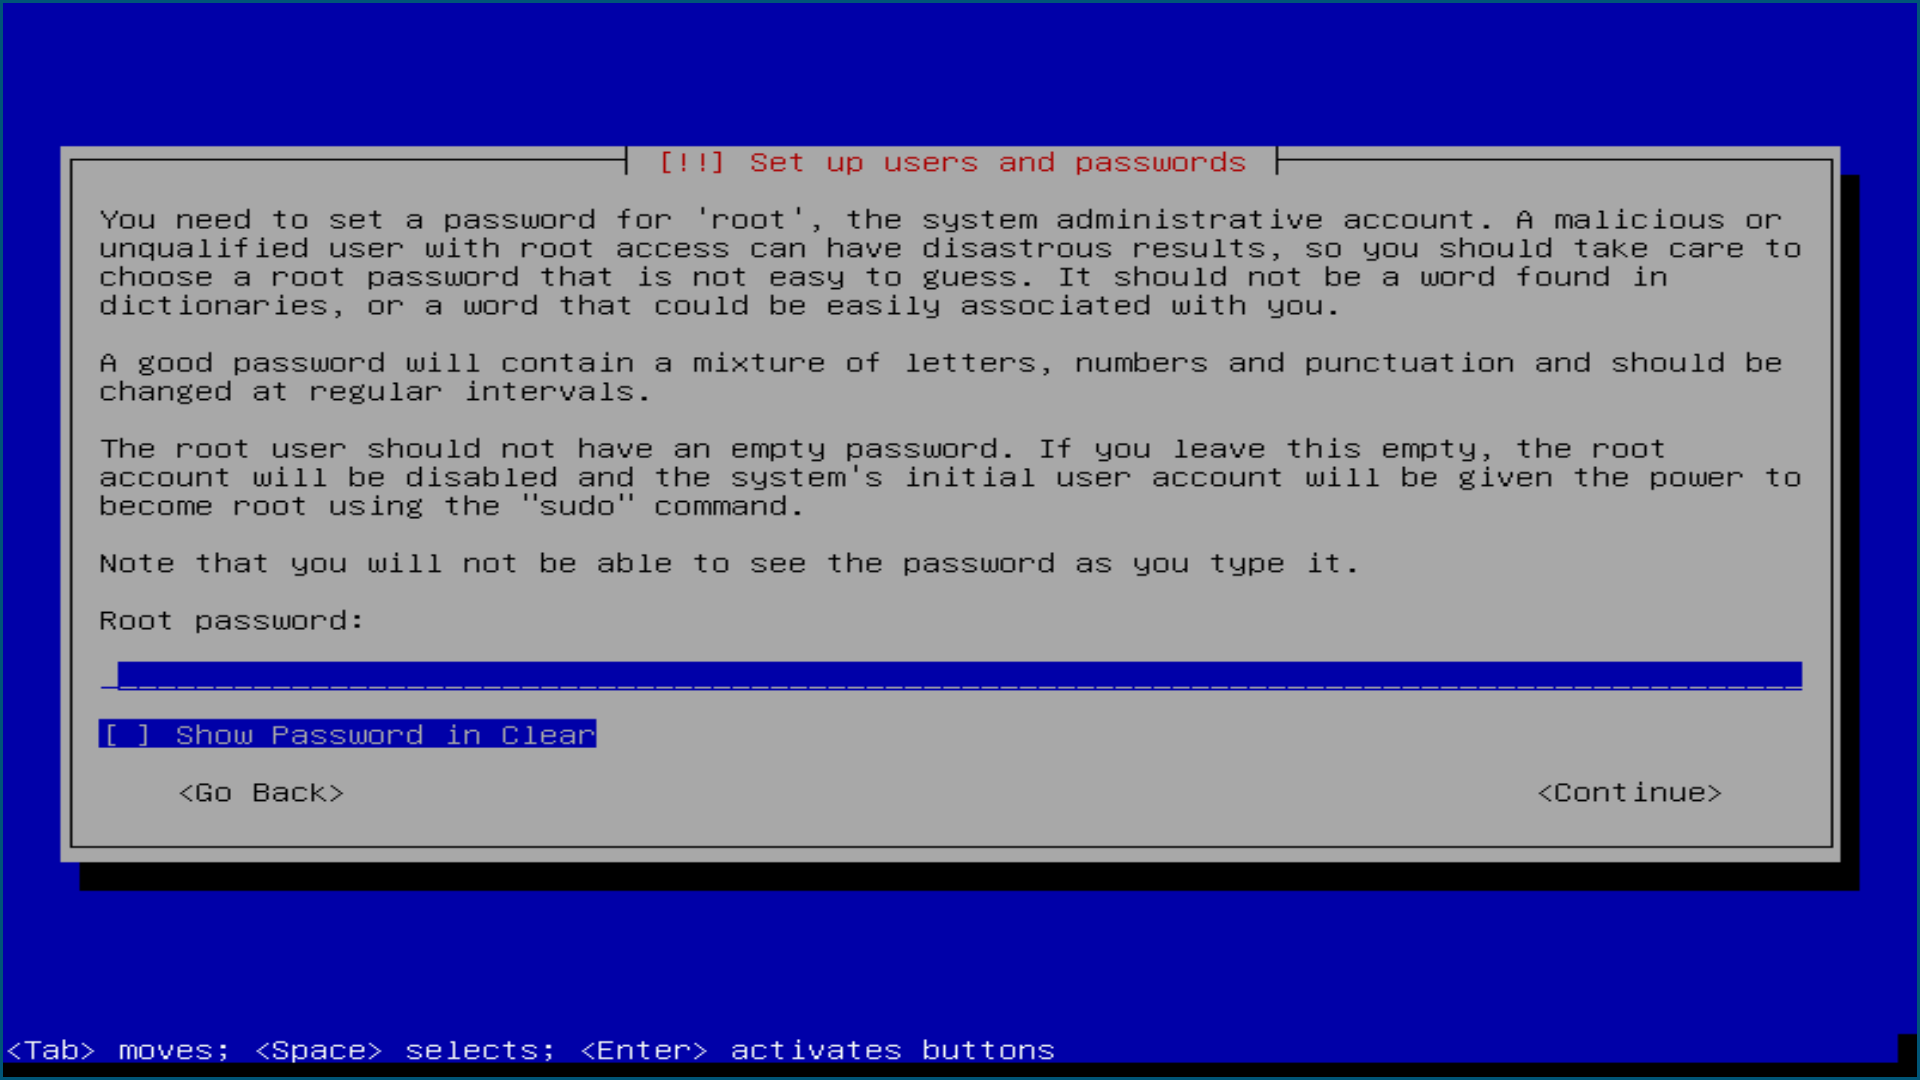
\includegraphics[width=.5\linewidth]{screenshots/08.png}
\end{center}

\begin{figure}[htbp]
\centering
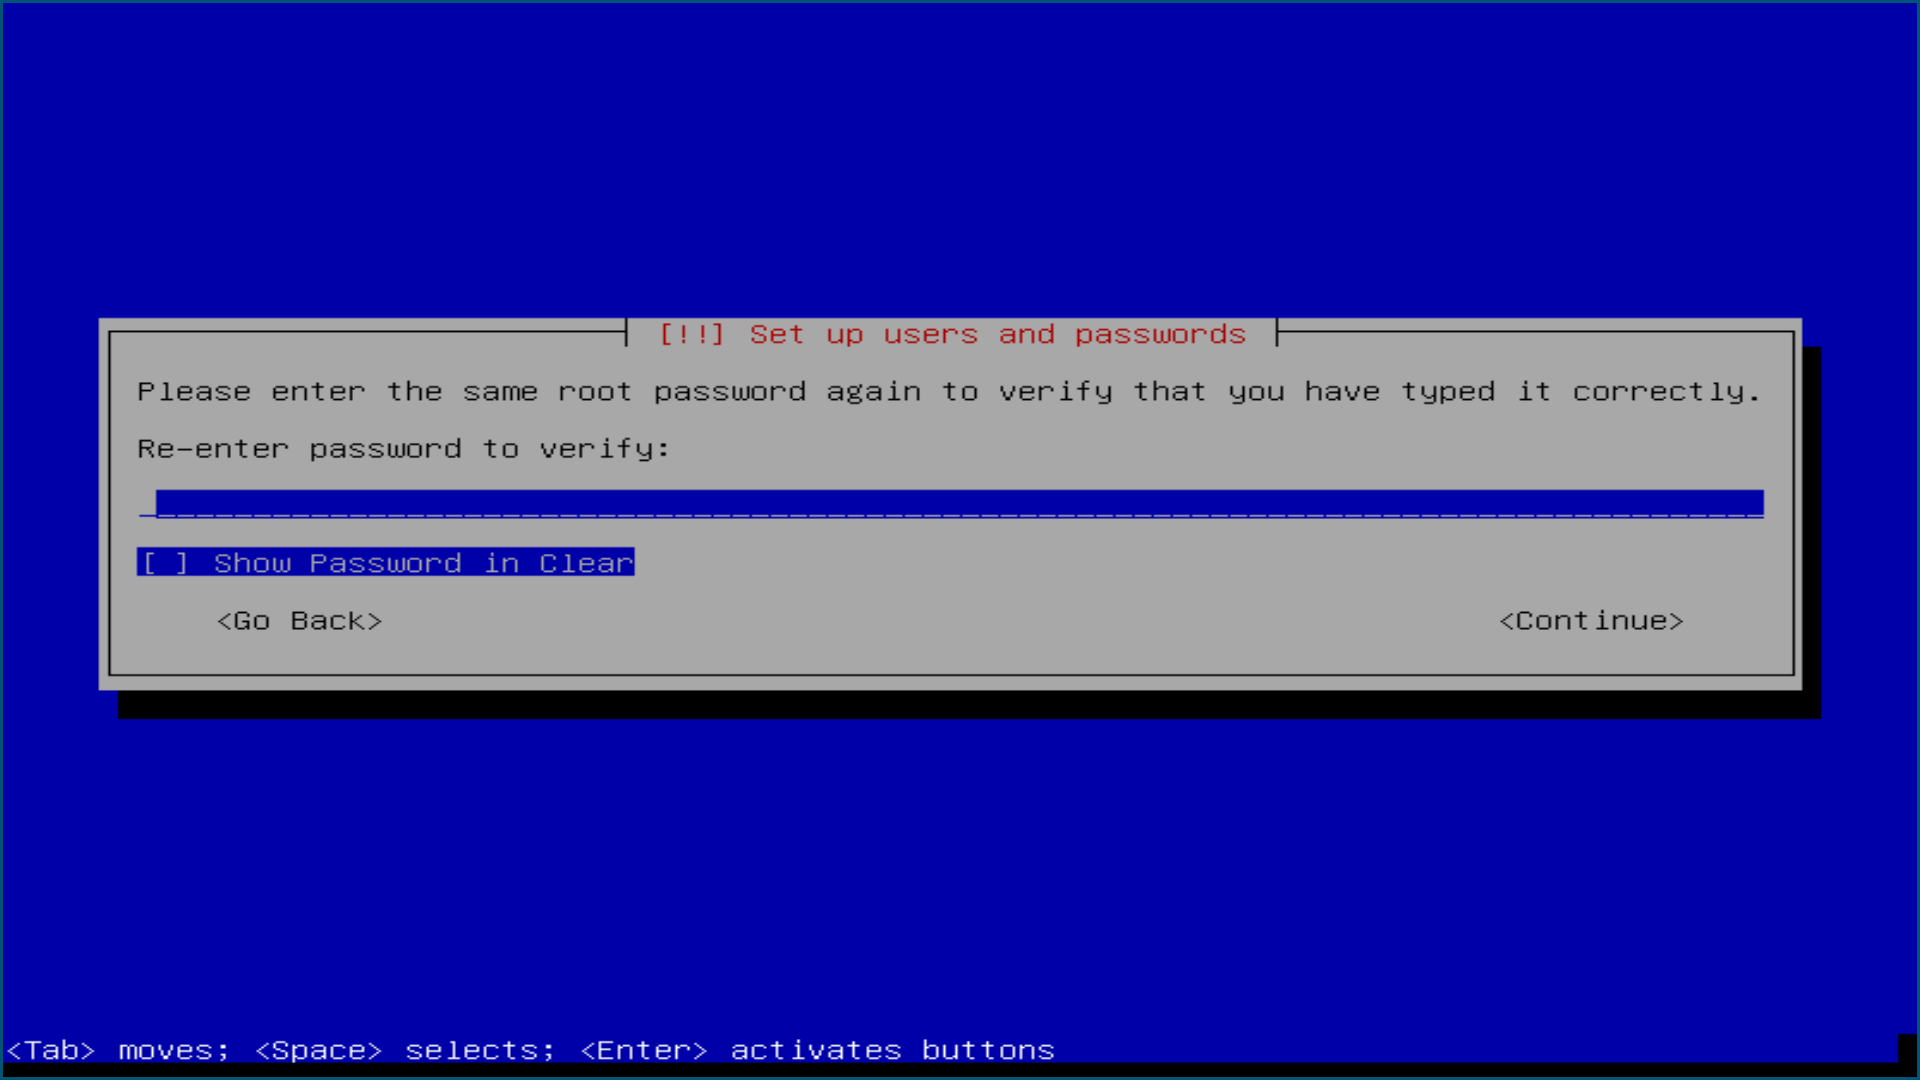
\includegraphics[width=.5\linewidth]{screenshots/09.png}
\caption{回车跳过}
\end{figure}

\item 你的全名,注意,不是用户名!这一步不重要,但也别胡填,老老实实写姓
名的全拼,姓、名之间应该有空格。

\begin{center}
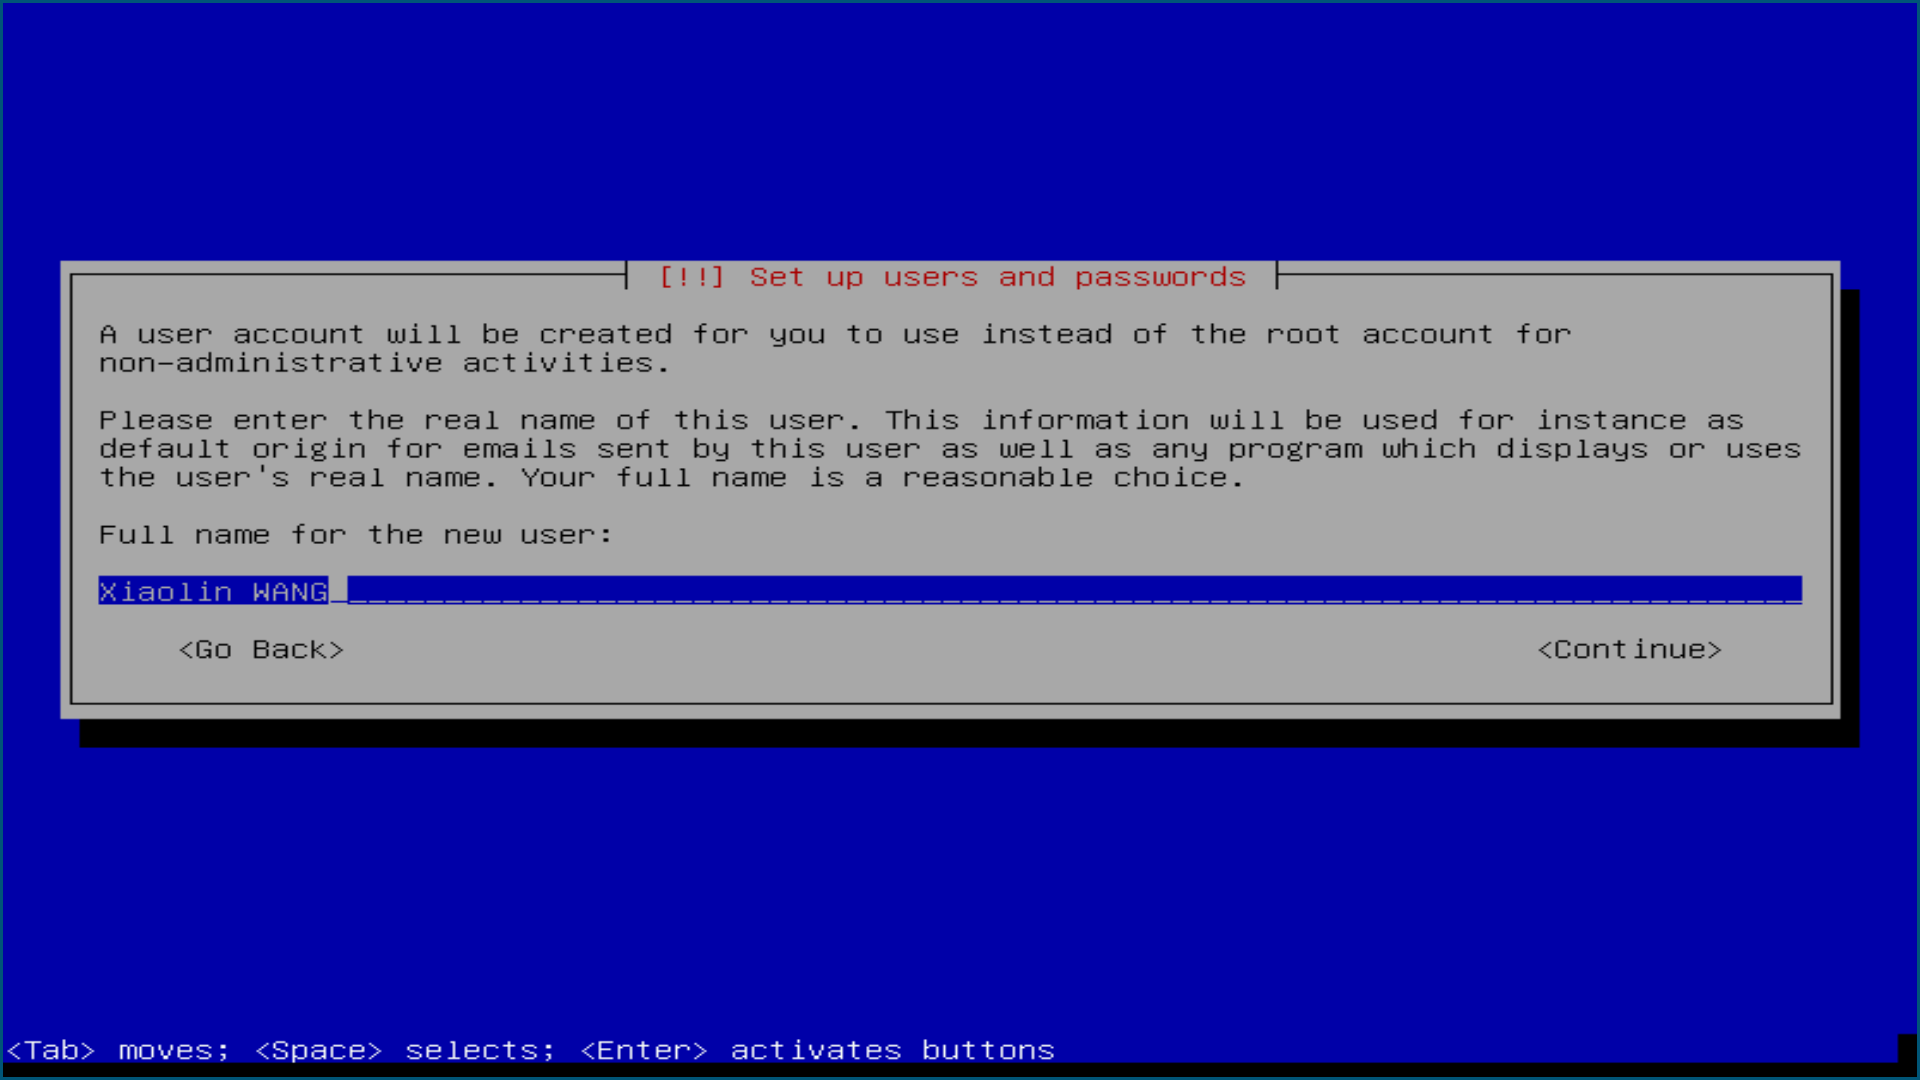
\includegraphics[width=.5\linewidth]{screenshots/10.png}
\end{center}

\item 用户名短点好,选个好记的

\begin{center}
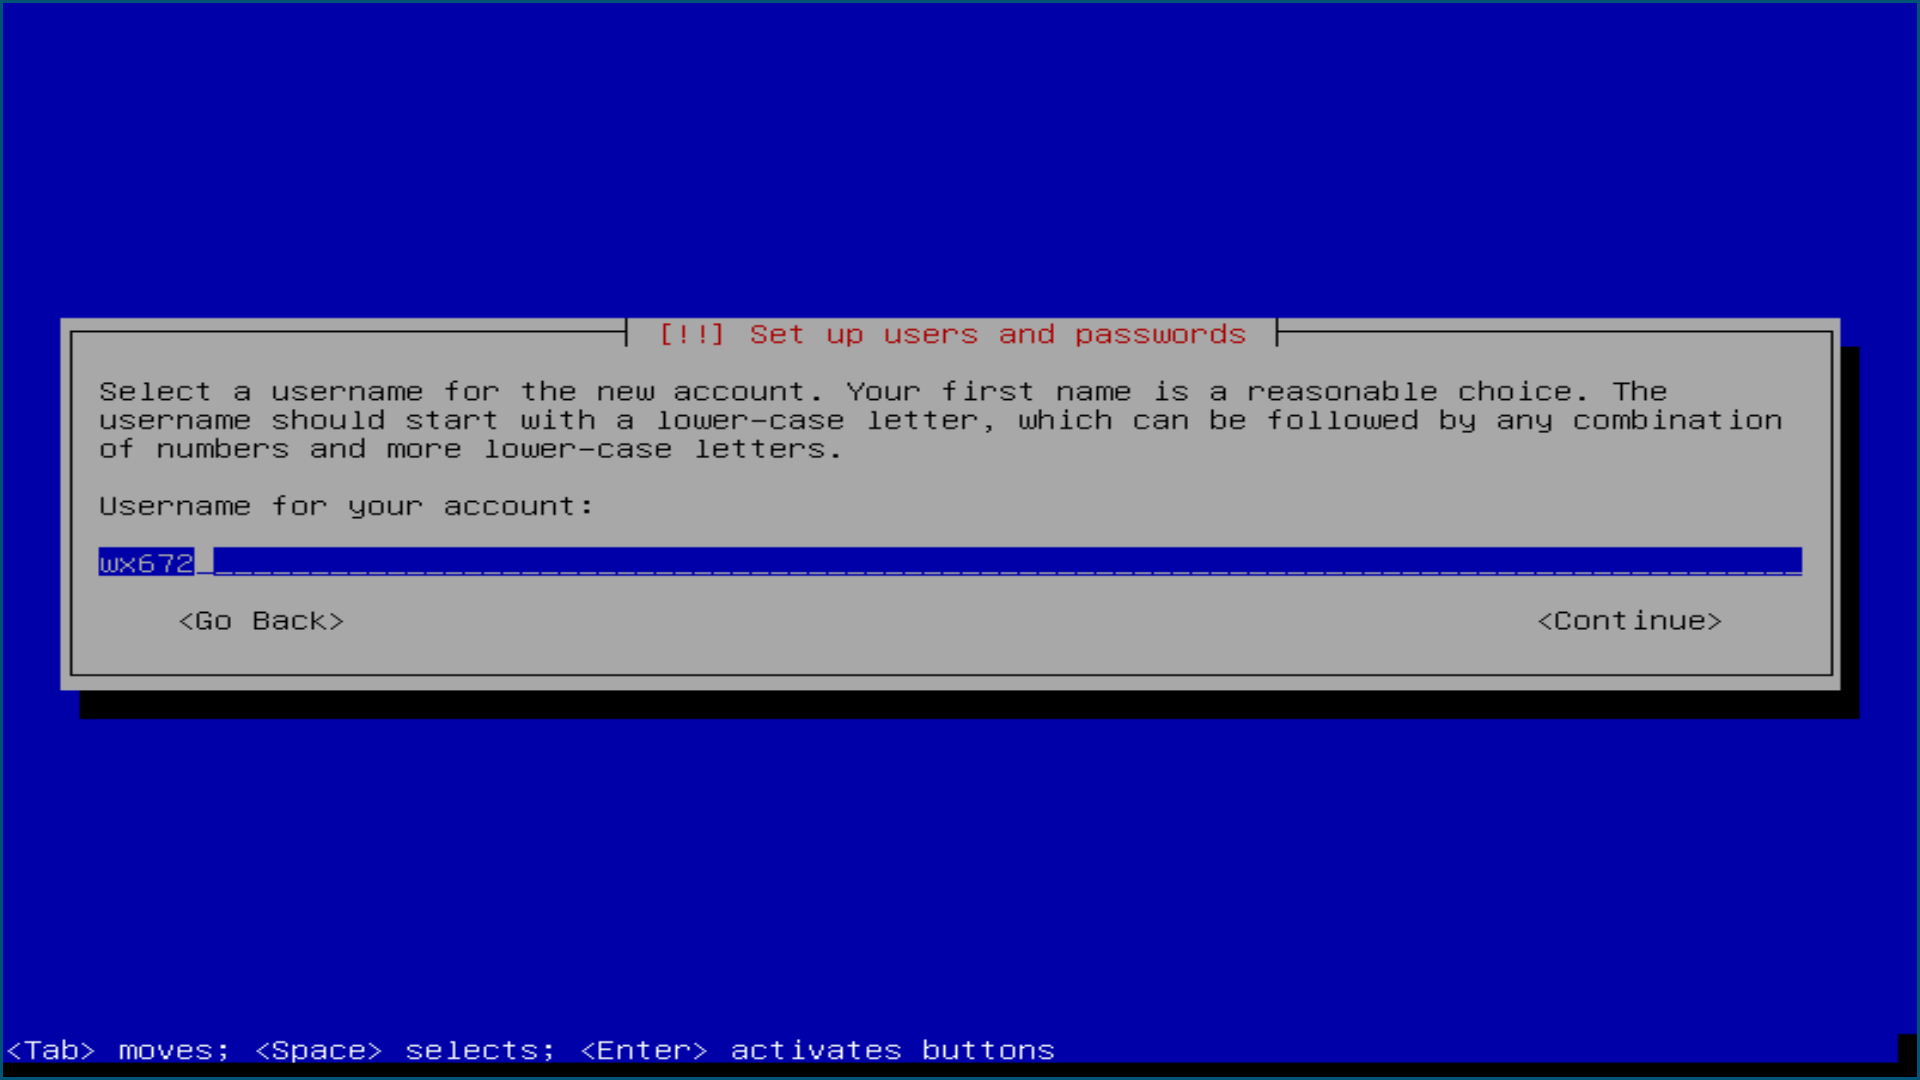
\includegraphics[width=.5\linewidth]{screenshots/11.png}
\end{center}

\item 密码,暂时选个短的,好记的

\begin{center}
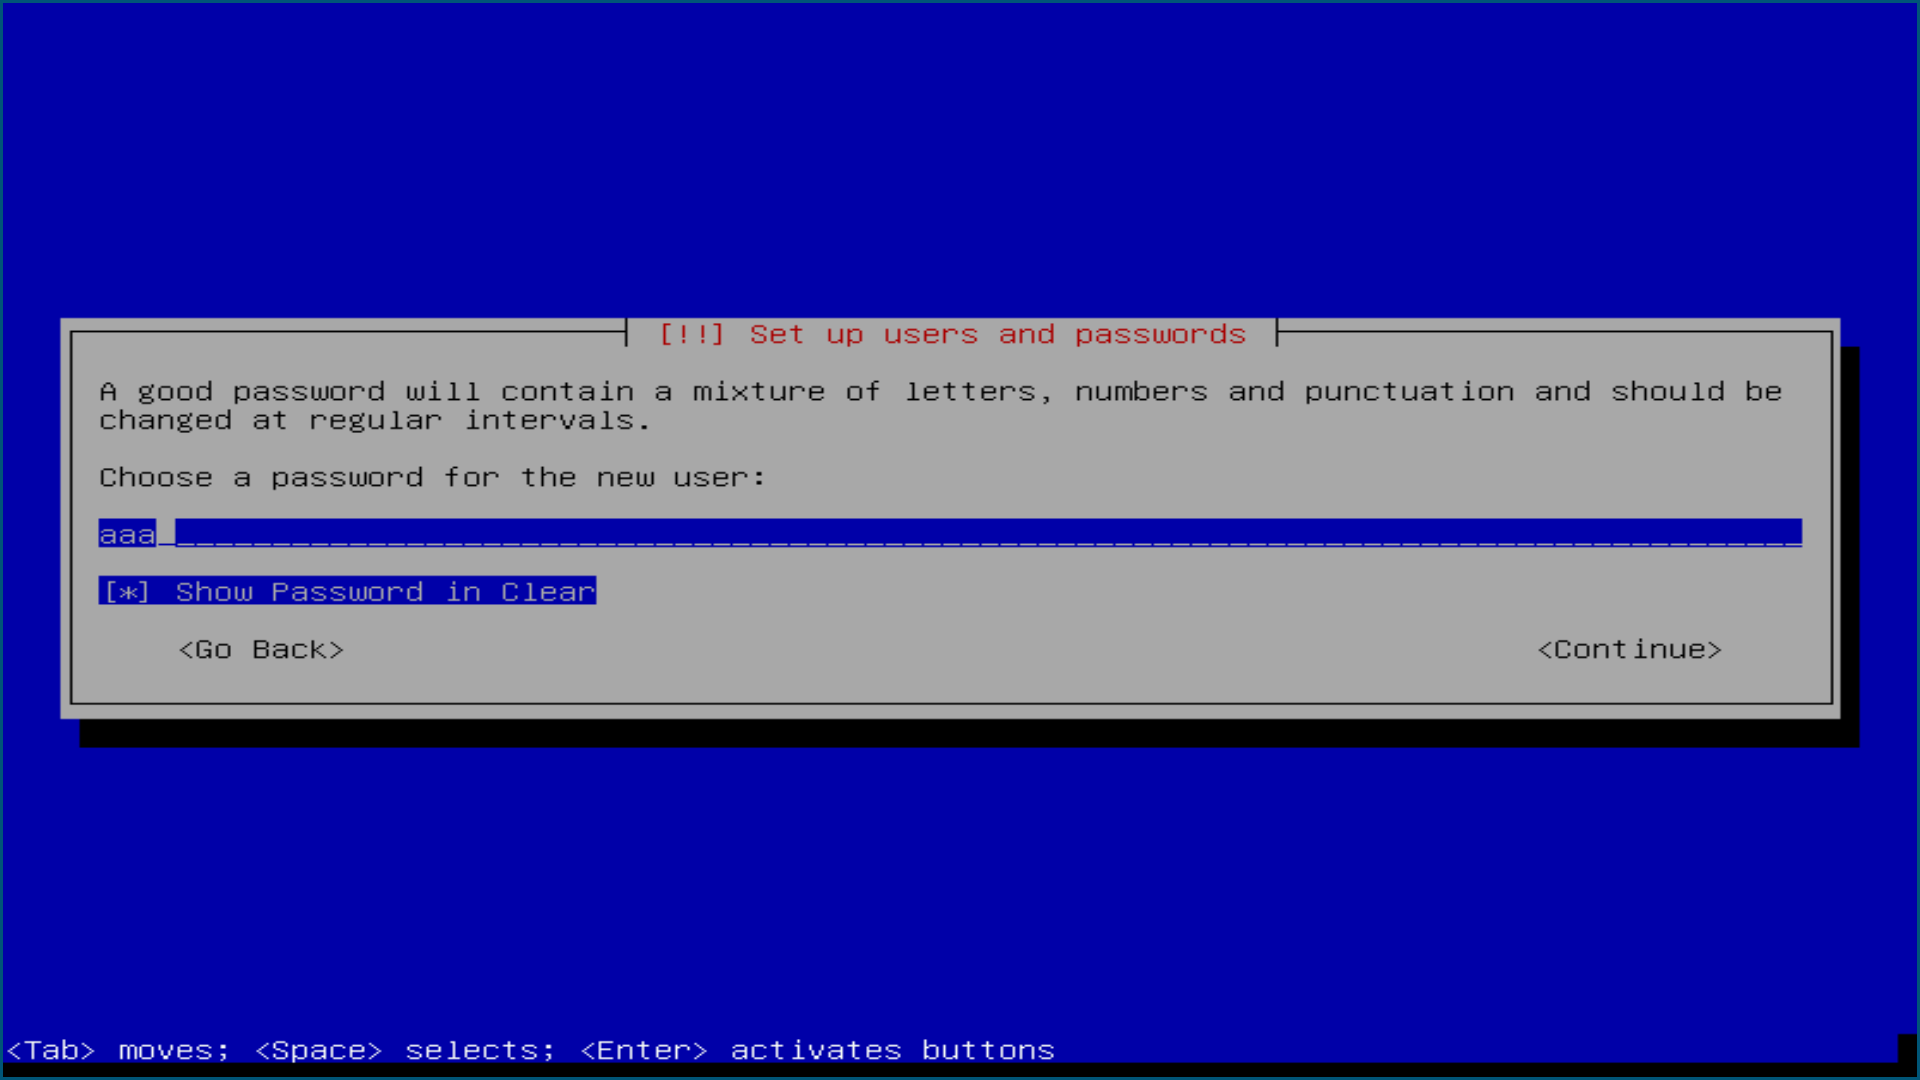
\includegraphics[width=.5\linewidth]{screenshots/12.png}
\end{center}

\begin{center}
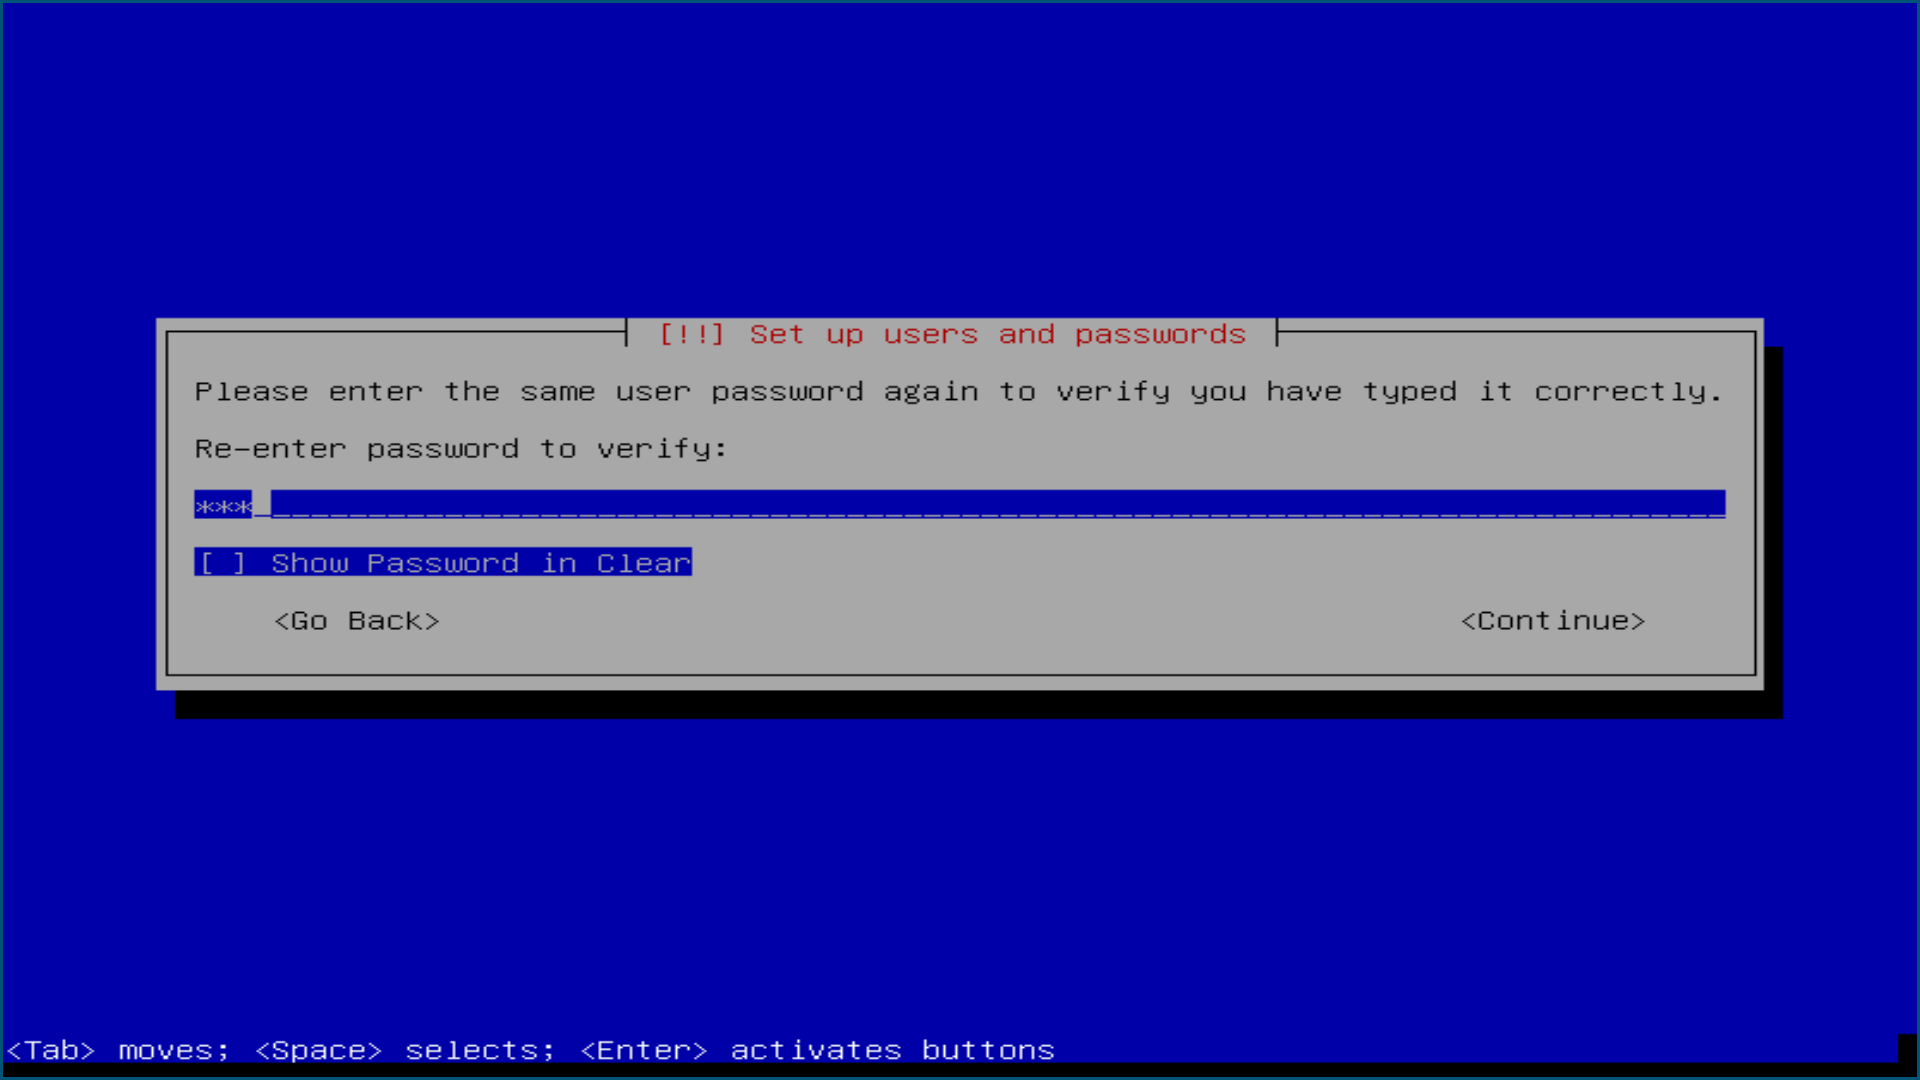
\includegraphics[width=.5\linewidth]{screenshots/13.png}
\end{center}

\item 选时区,暂时不重要,回车接受默认值就好

\begin{center}
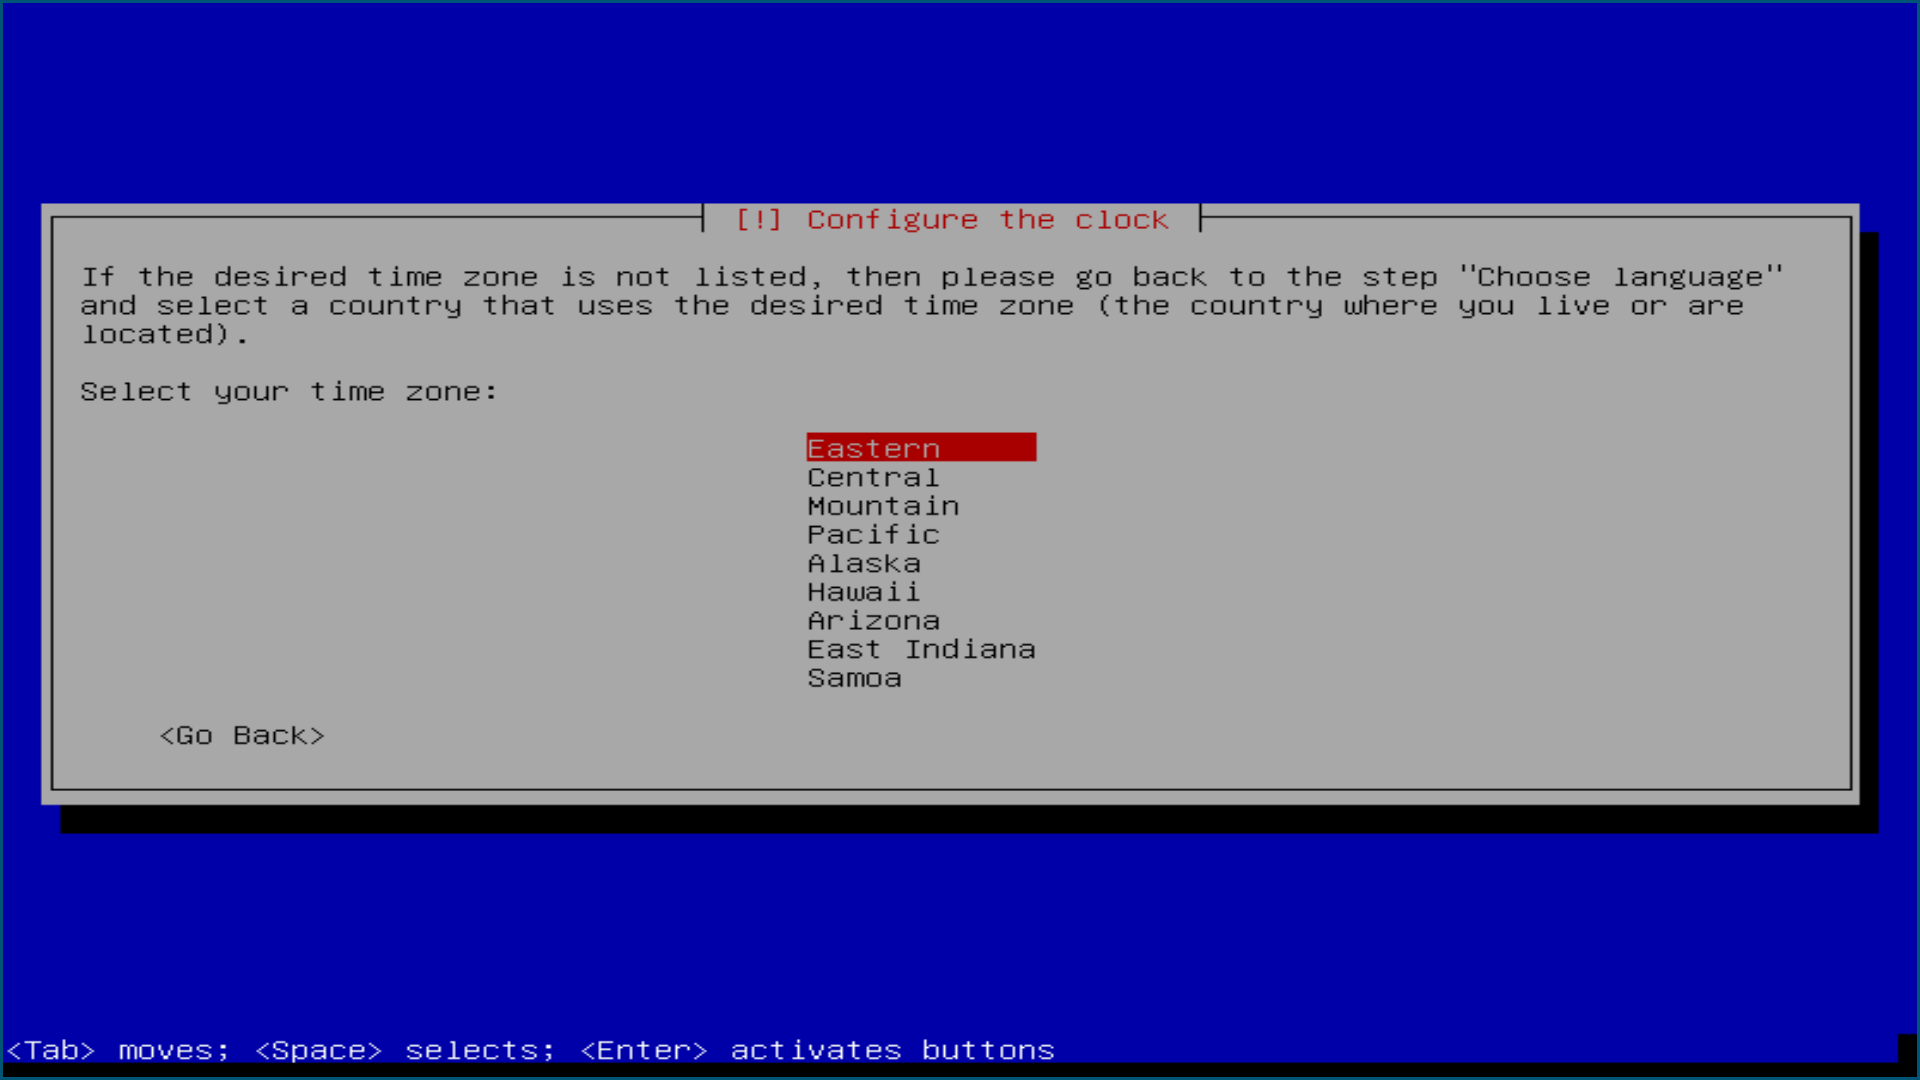
\includegraphics[width=.5\linewidth]{screenshots/14.png}
\end{center}

\item 硬盘分区,很重要!

\begin{itemize}
\item 如果像我一样,你也是装Linux单系统的话,选“Guided - use entire
disk”;

\item 如果是装双系统,就选“Manual”。

\begin{center}
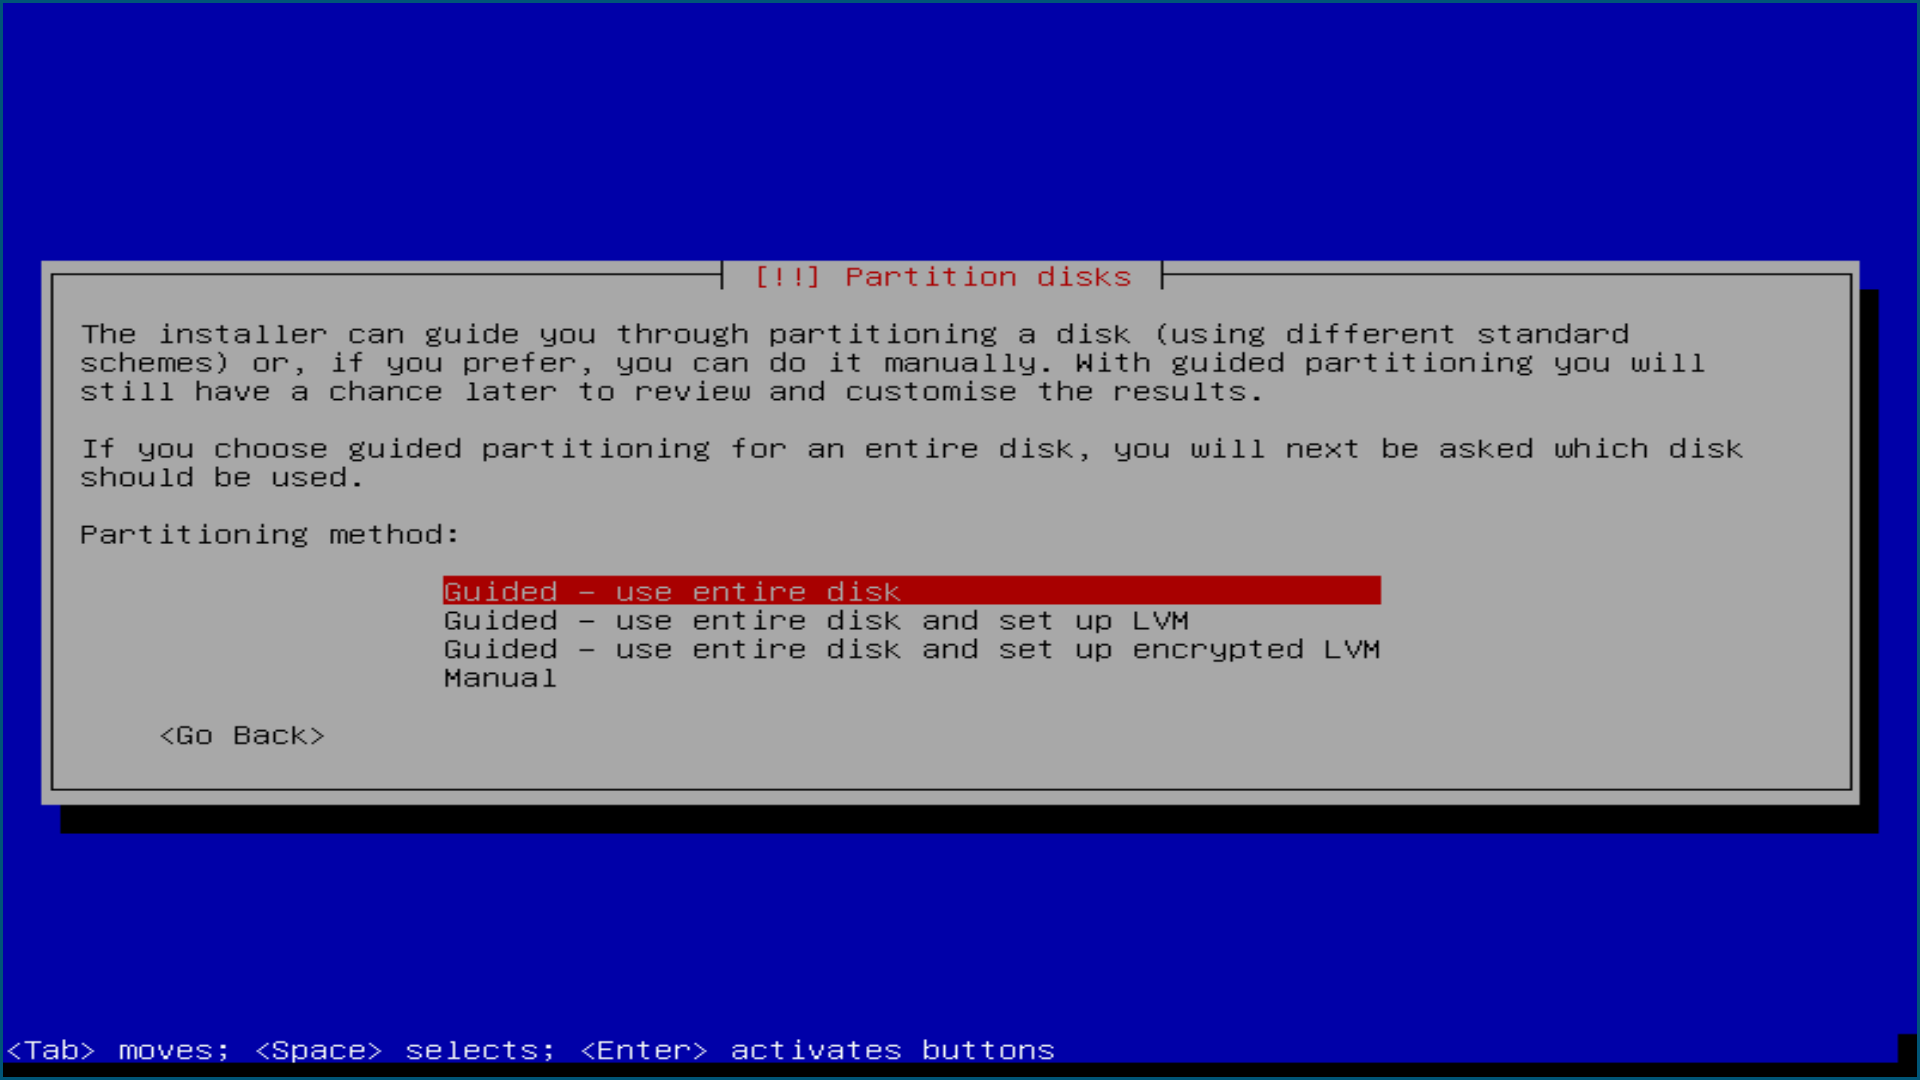
\includegraphics[width=.5\linewidth]{screenshots/15.png}
\end{center}

\begin{figure}[htbp]
\centering
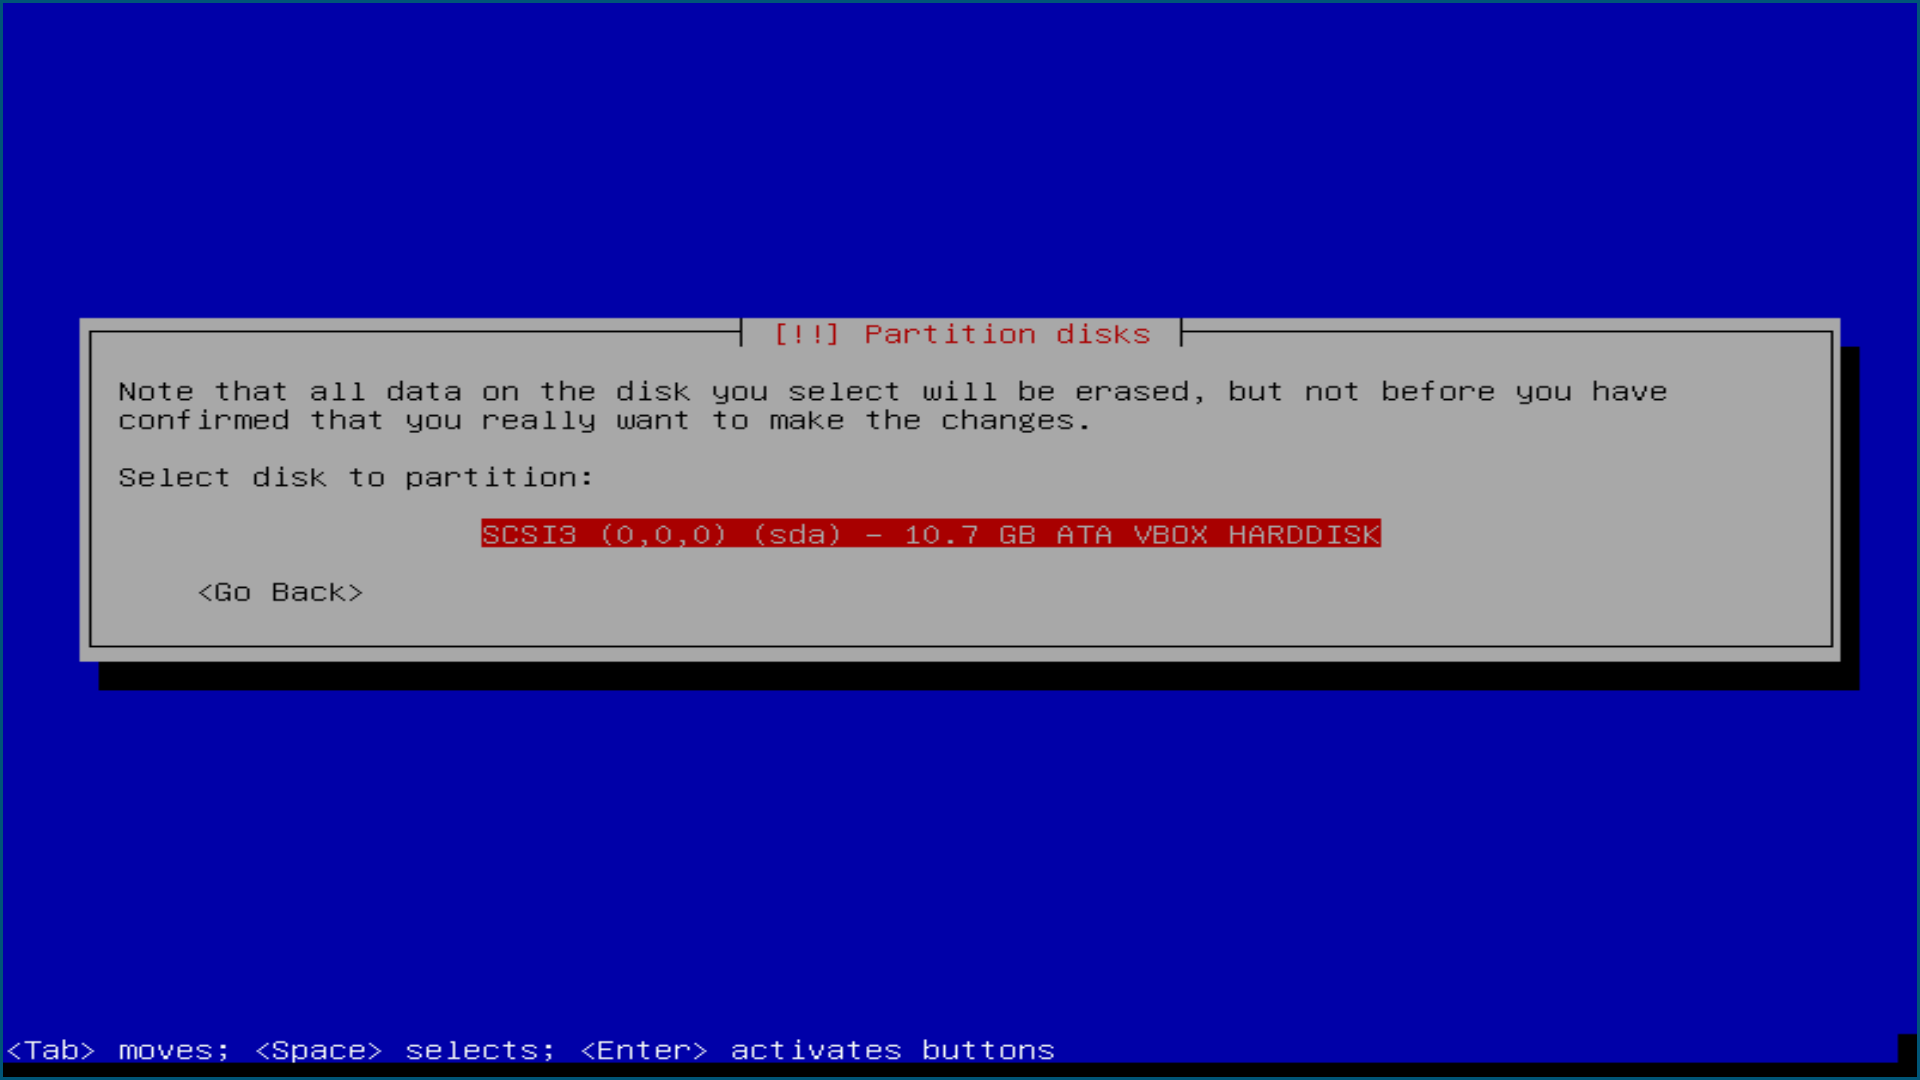
\includegraphics[width=.5\linewidth]{screenshots/16.png}
\caption{选择要分区的硬盘。我只有一块硬盘,你可未必,别选错!}
\end{figure}

\begin{figure}[htbp]
\centering
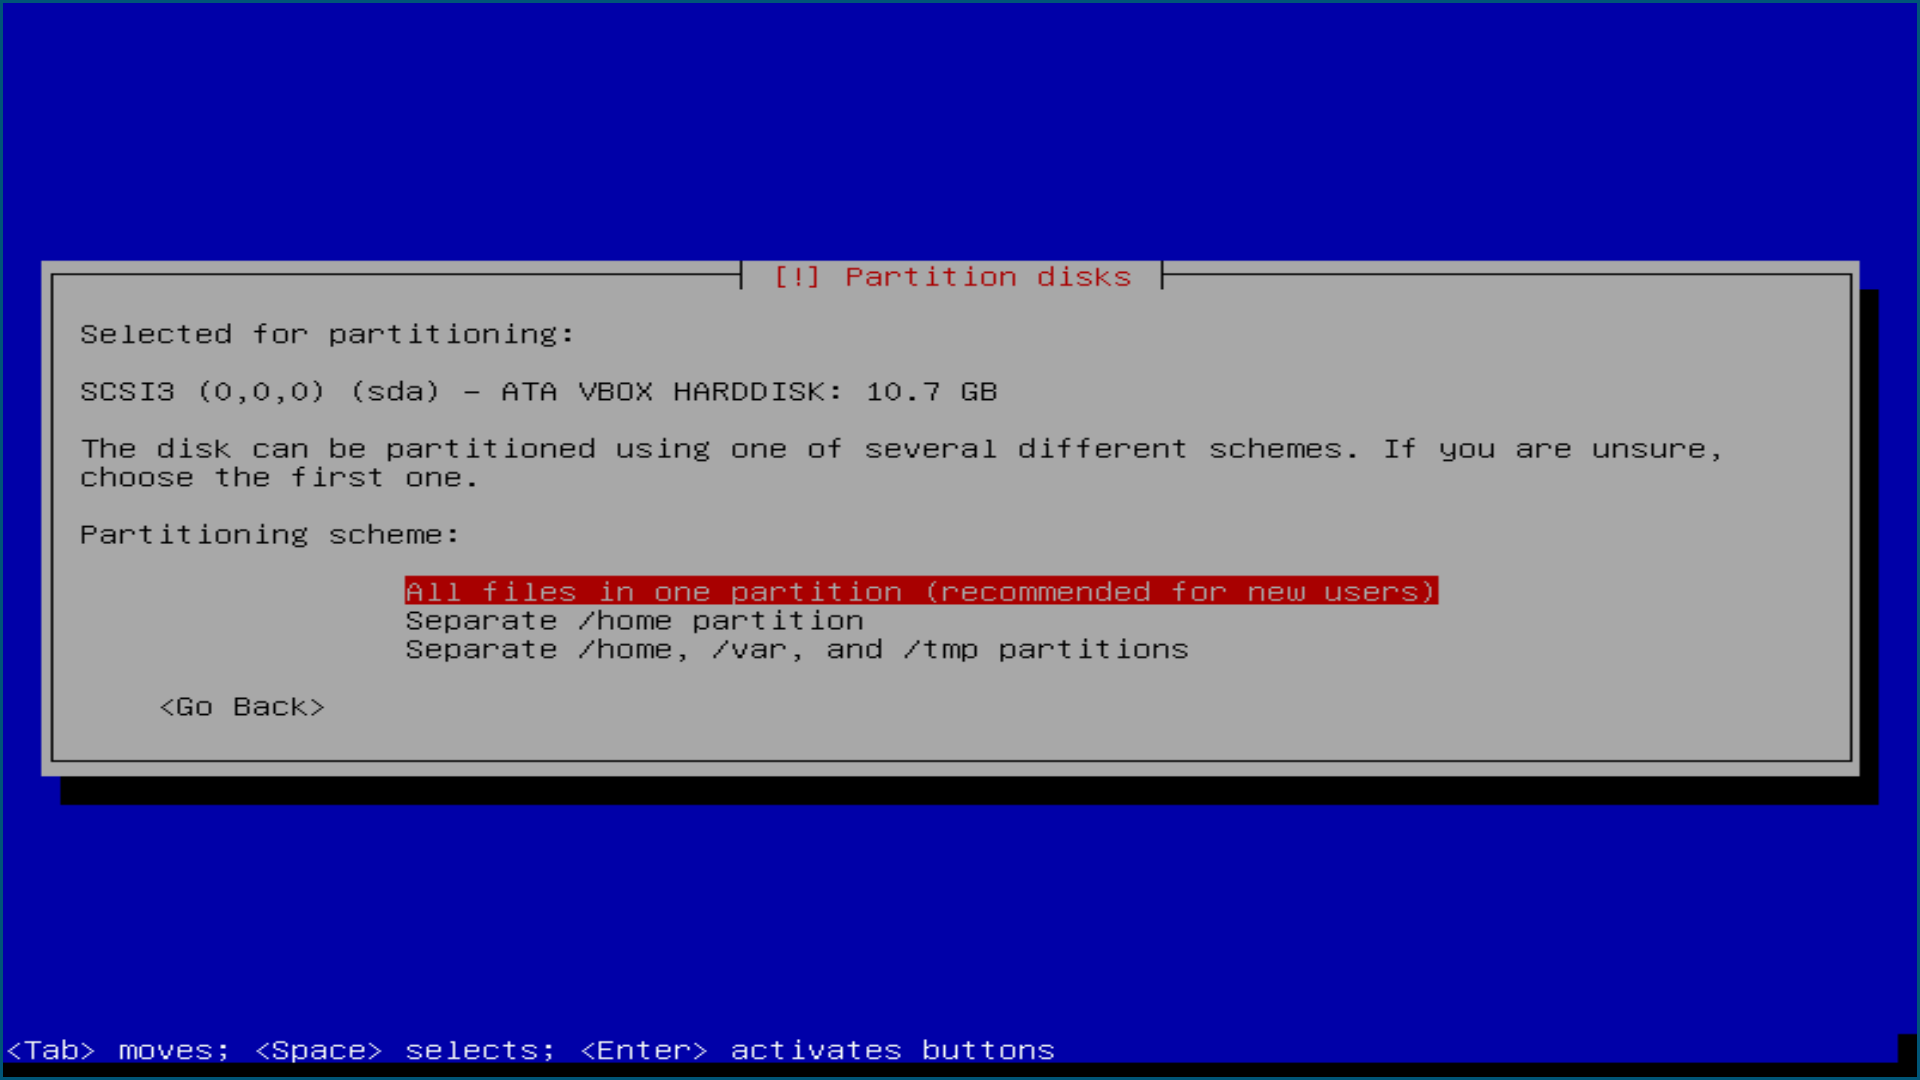
\includegraphics[width=.5\linewidth]{screenshots/17.png}
\caption{分区规划。装单系统的话,很简单,选择“All files in one partition”就好。如果你是装双系统,也就是说在前面选择了“Manual”,那么这里的事情会稍复杂一点,你要自己创建一个1GB大小的“swap分区”,再把剩下的空间都用作“根分区”。}
\end{figure}

\begin{figure}[htbp]
\centering
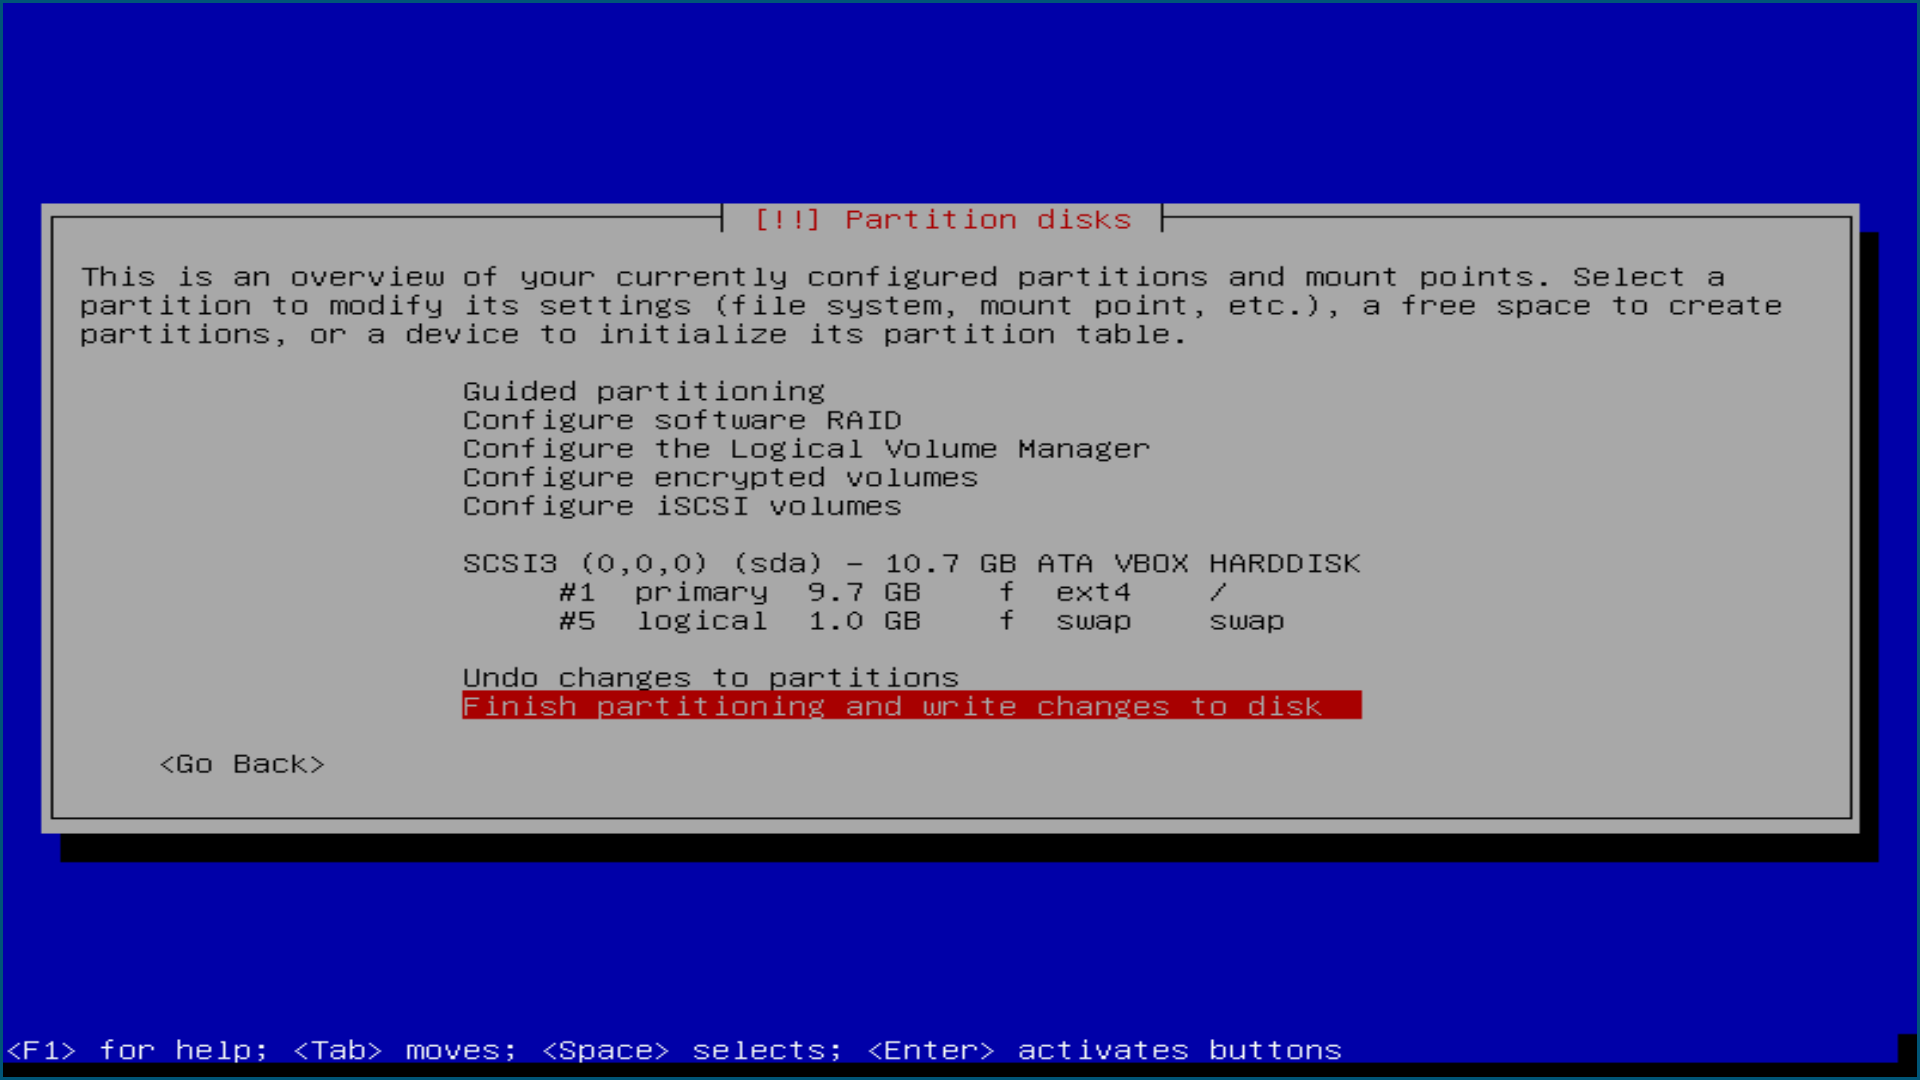
\includegraphics[width=.5\linewidth]{screenshots/18.png}
\caption{一个1GB的swap分区和一个根分区(/)}
\end{figure}

\begin{figure}[htbp]
\centering
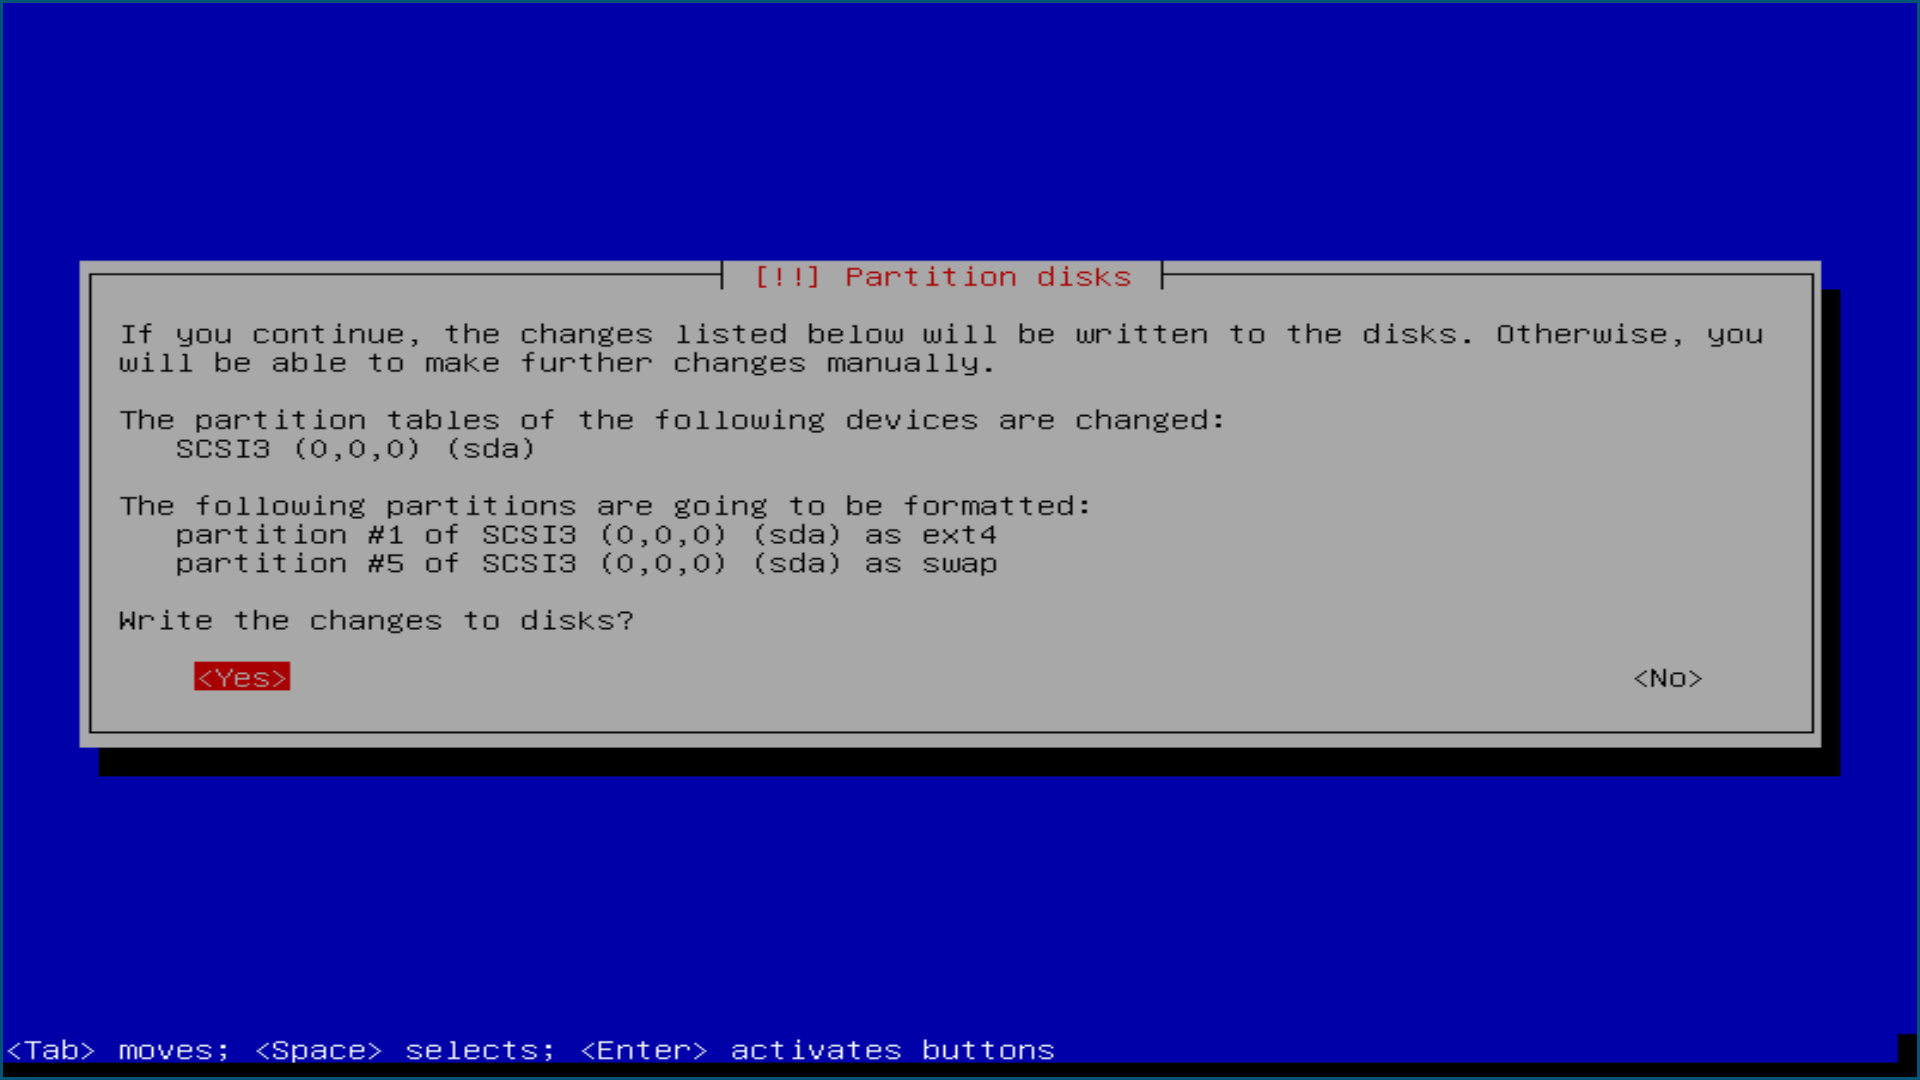
\includegraphics[width=.5\linewidth]{screenshots/19.png}
\caption{当然选“Yes”,如果硬盘上原来的数据都备份好了。}
\end{figure}
\end{itemize}

\item 开始安装最小系统,大概5分钟

\begin{center}
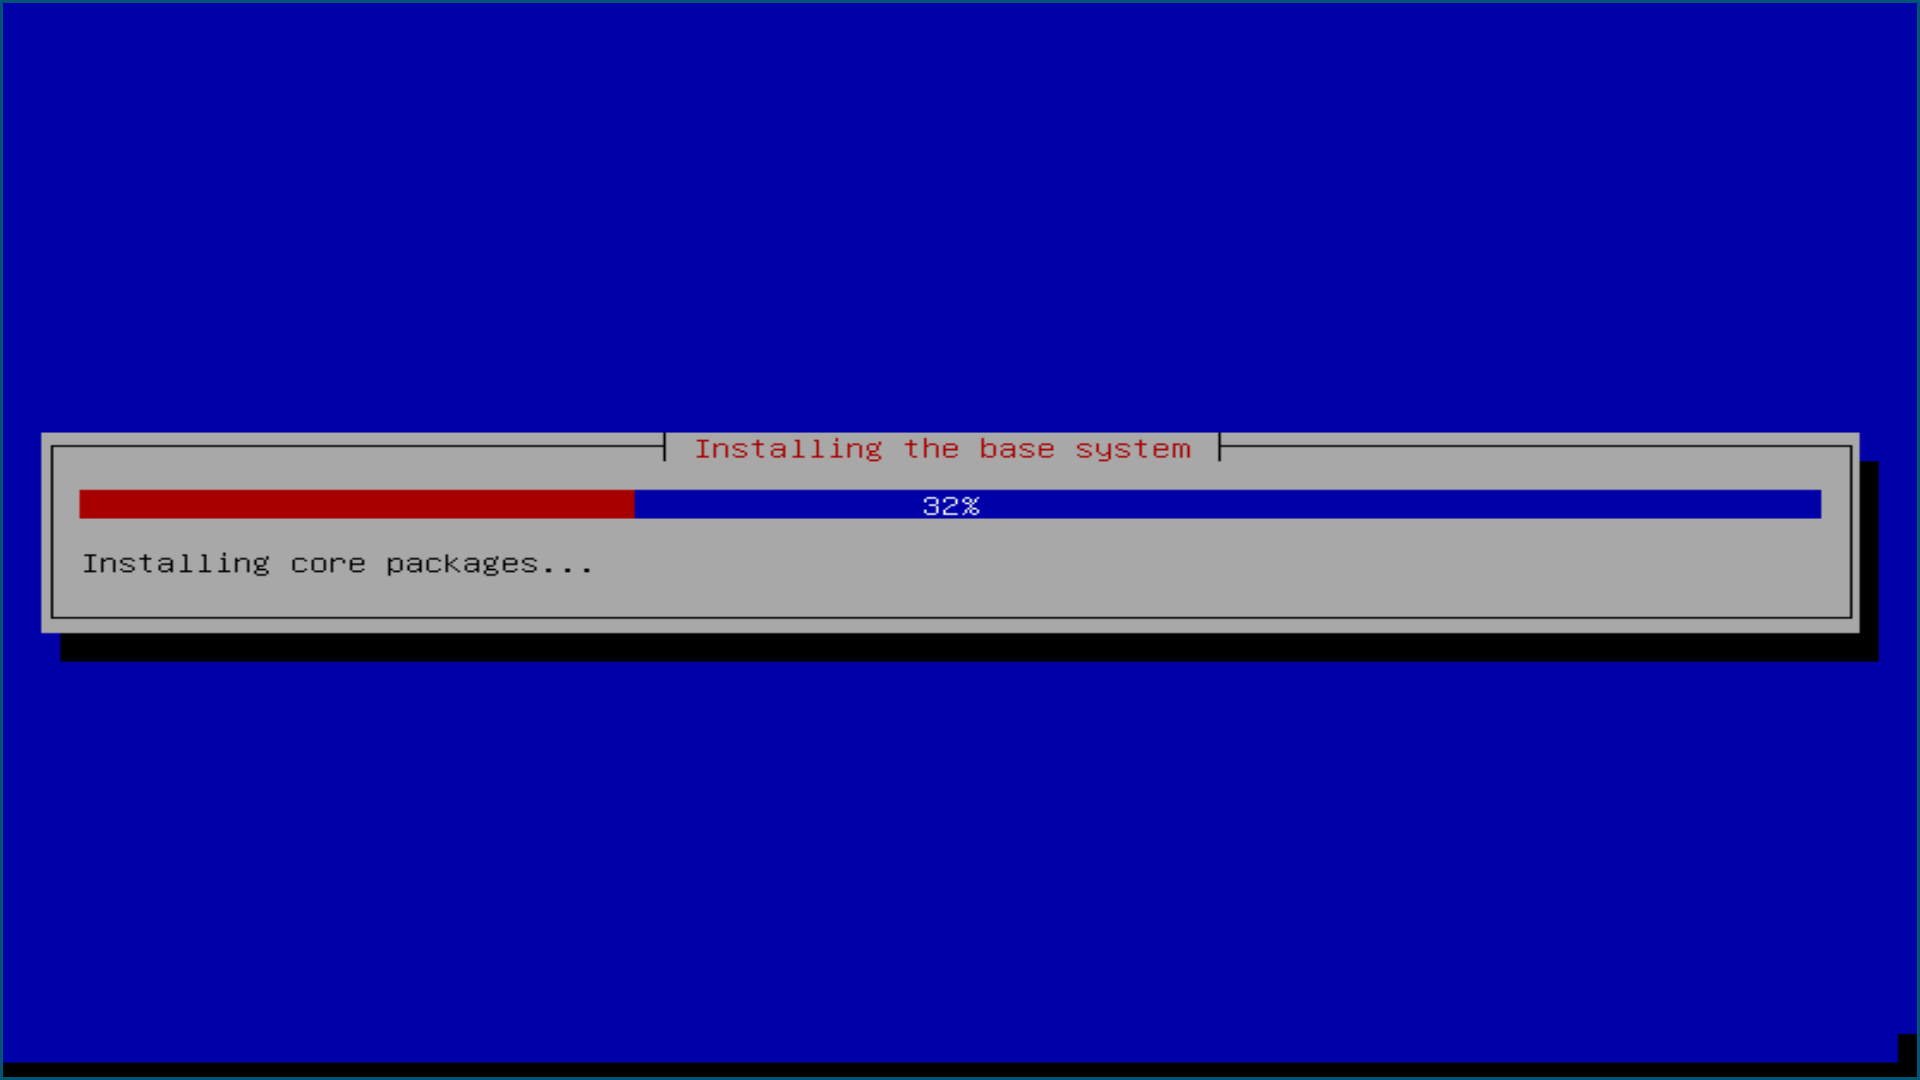
\includegraphics[width=.5\linewidth]{screenshots/20.png}
\end{center}

\begin{figure}[htbp]
\centering
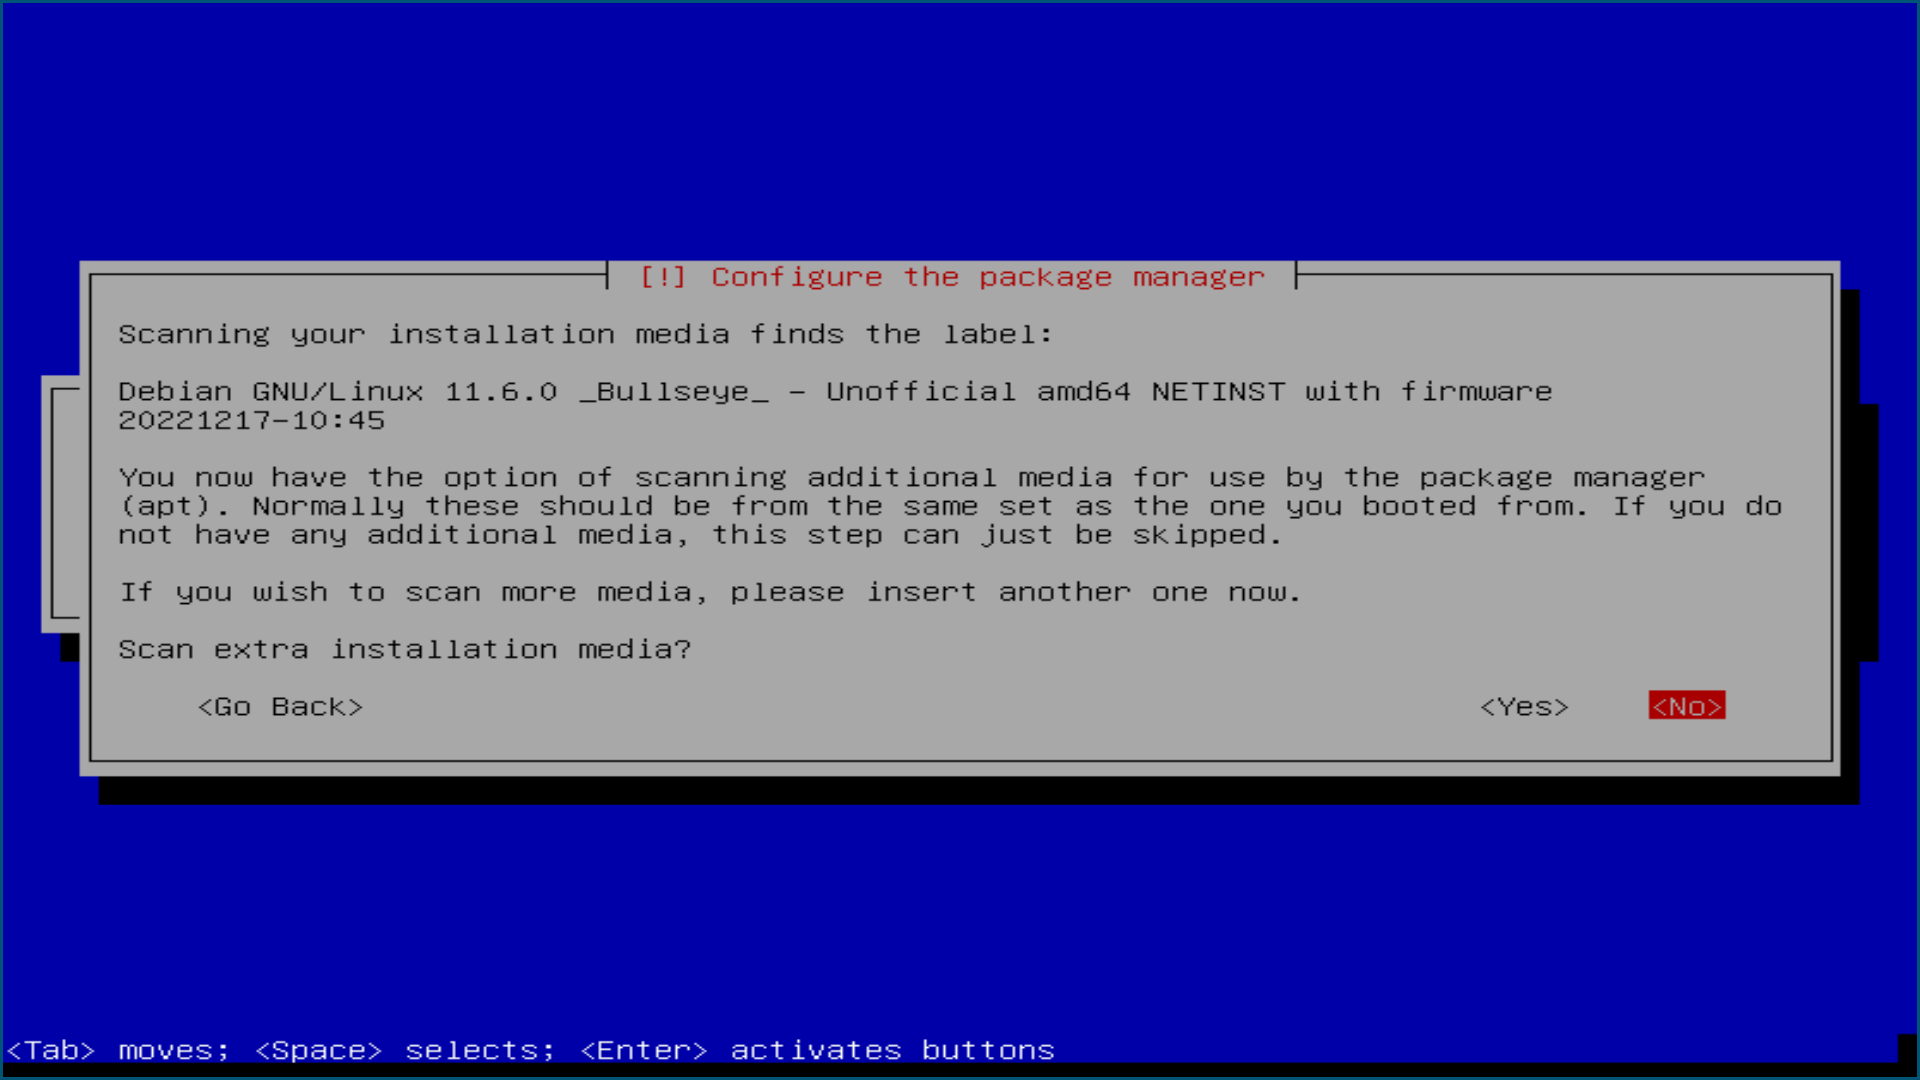
\includegraphics[width=.5\linewidth]{screenshots/21.png}
\caption{配置package manager,选“No”}
\end{figure}

\begin{figure}[htbp]
\centering
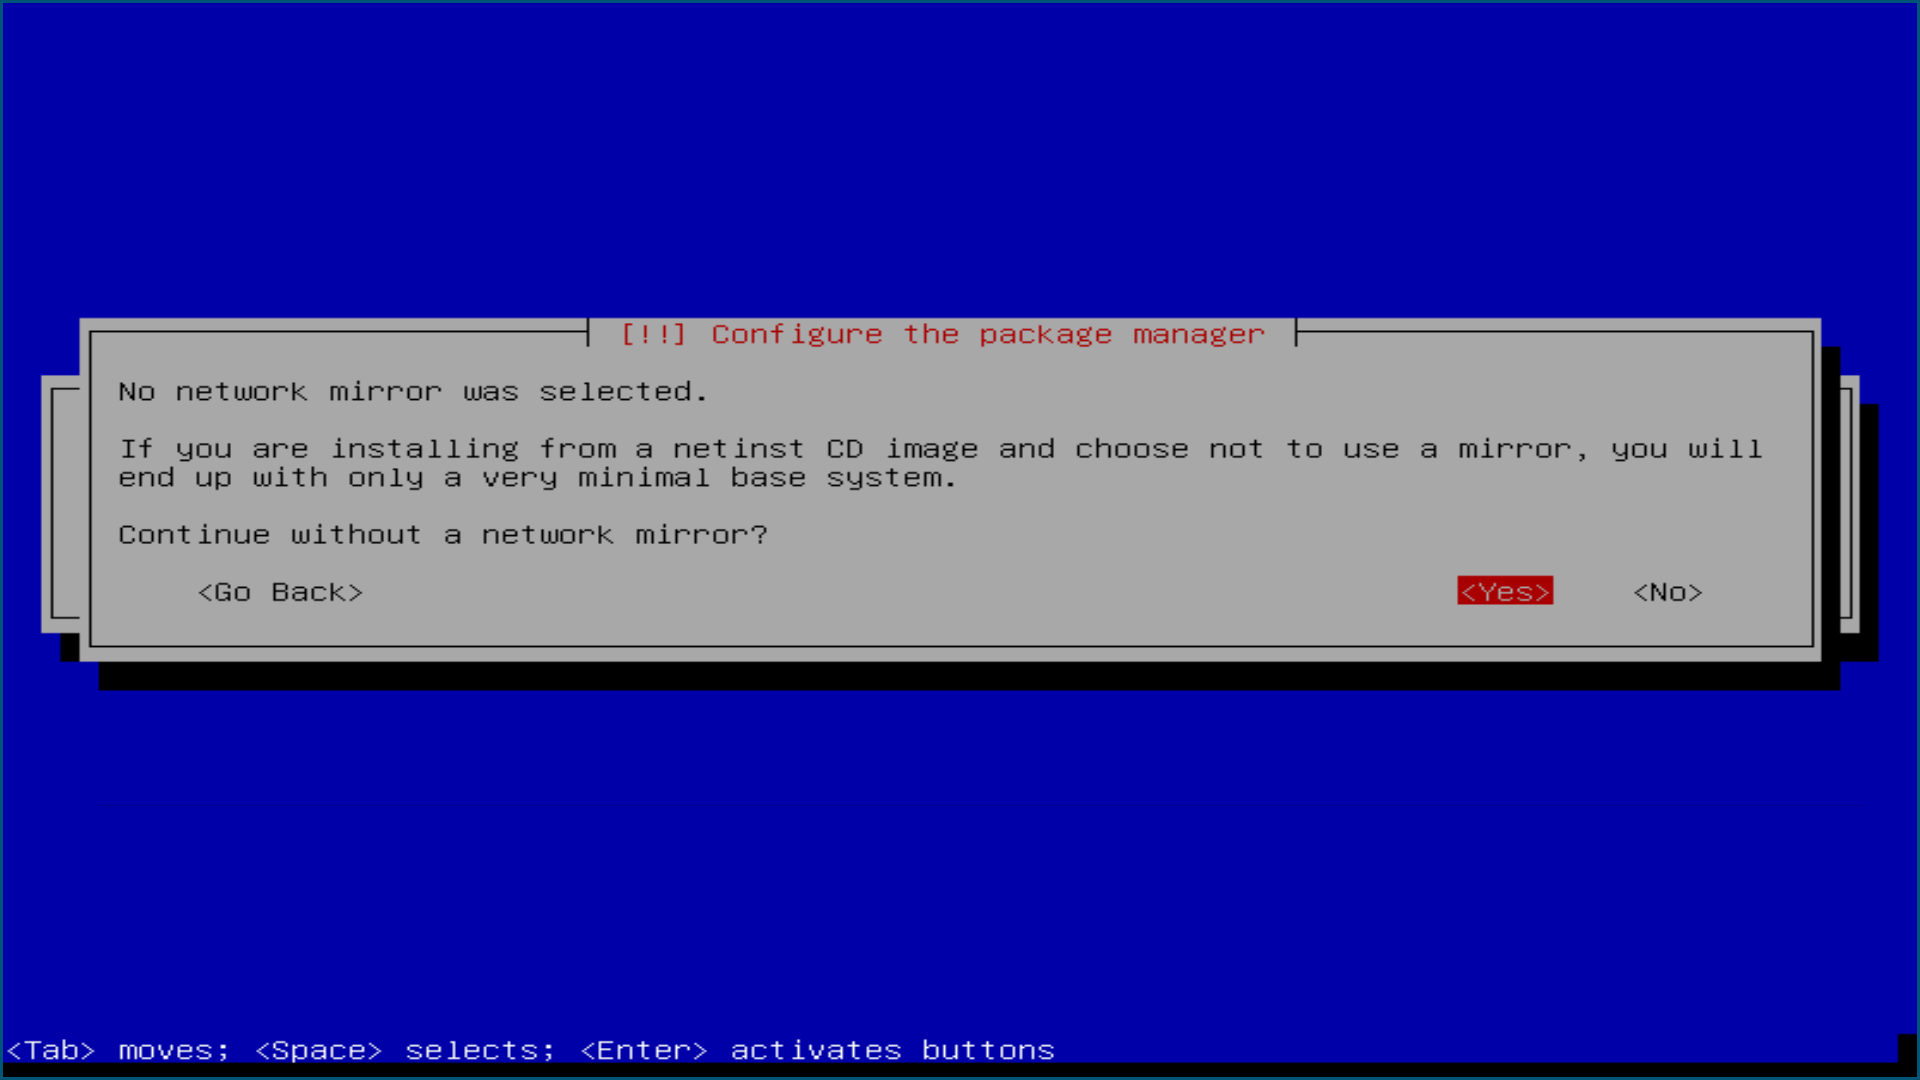
\includegraphics[width=.5\linewidth]{screenshots/22.png}
\caption{选“Yes”,因为我们没联网。}
\end{figure}

\begin{figure}[htbp]
\centering
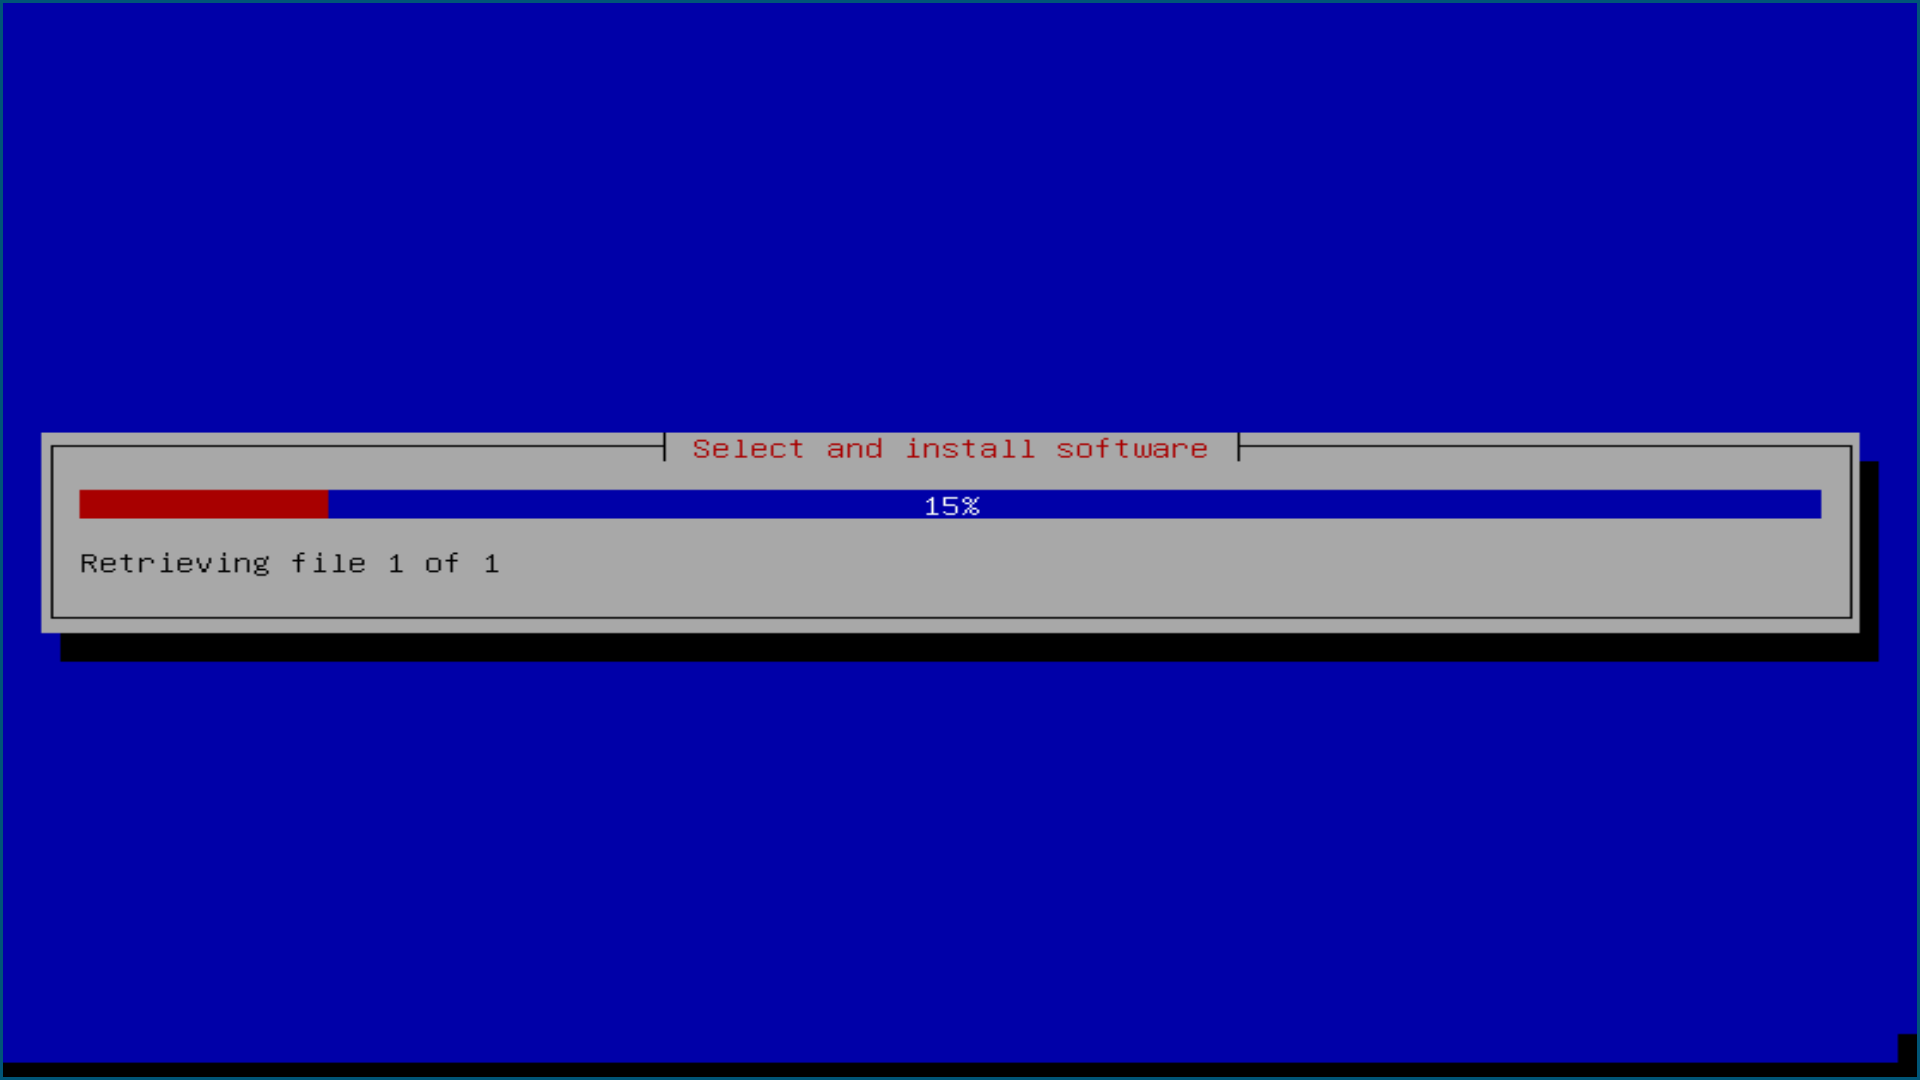
\includegraphics[width=.5\linewidth]{screenshots/23.png}
\caption{大概需要5分钟}
\end{figure}

\begin{figure}[htbp]
\centering
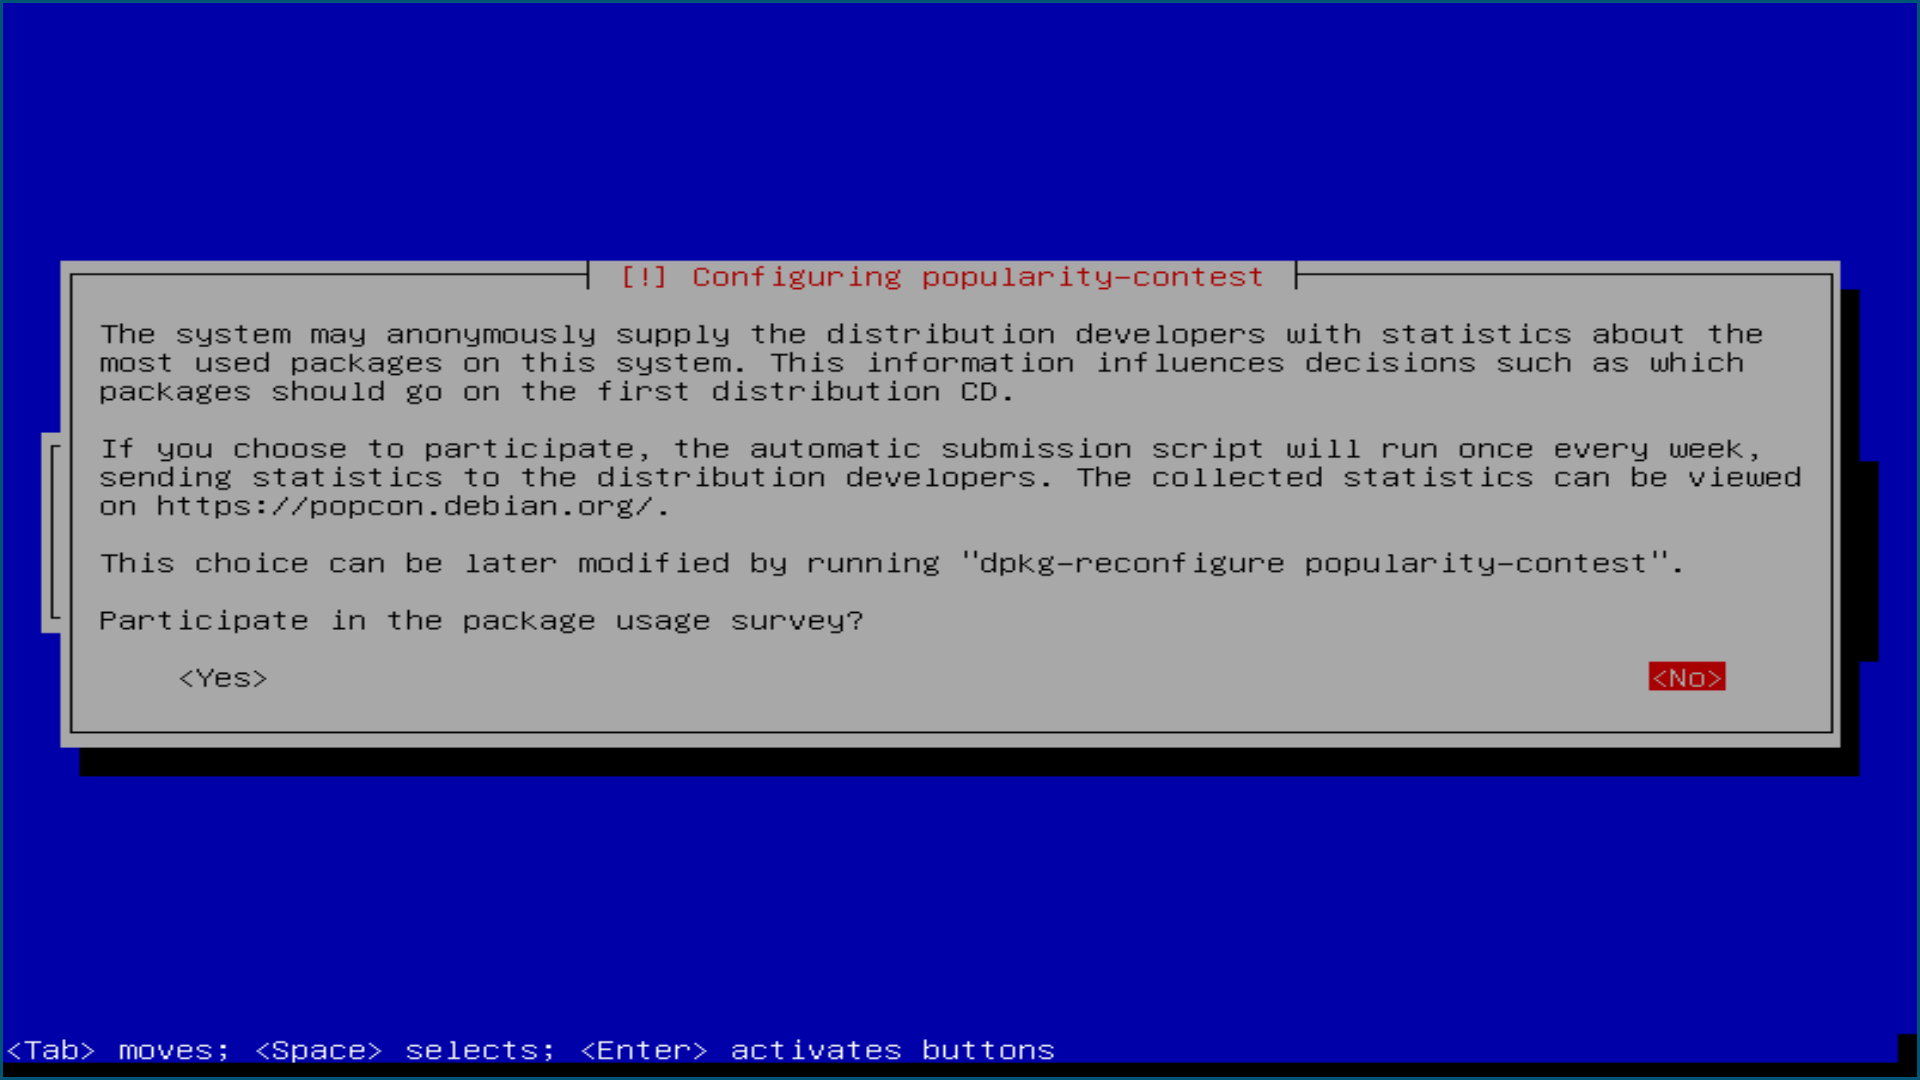
\includegraphics[width=.5\linewidth]{screenshots/24.png}
\caption{不重要,回车接受默认值就好}
\end{figure}

\begin{figure}[htbp]
\centering
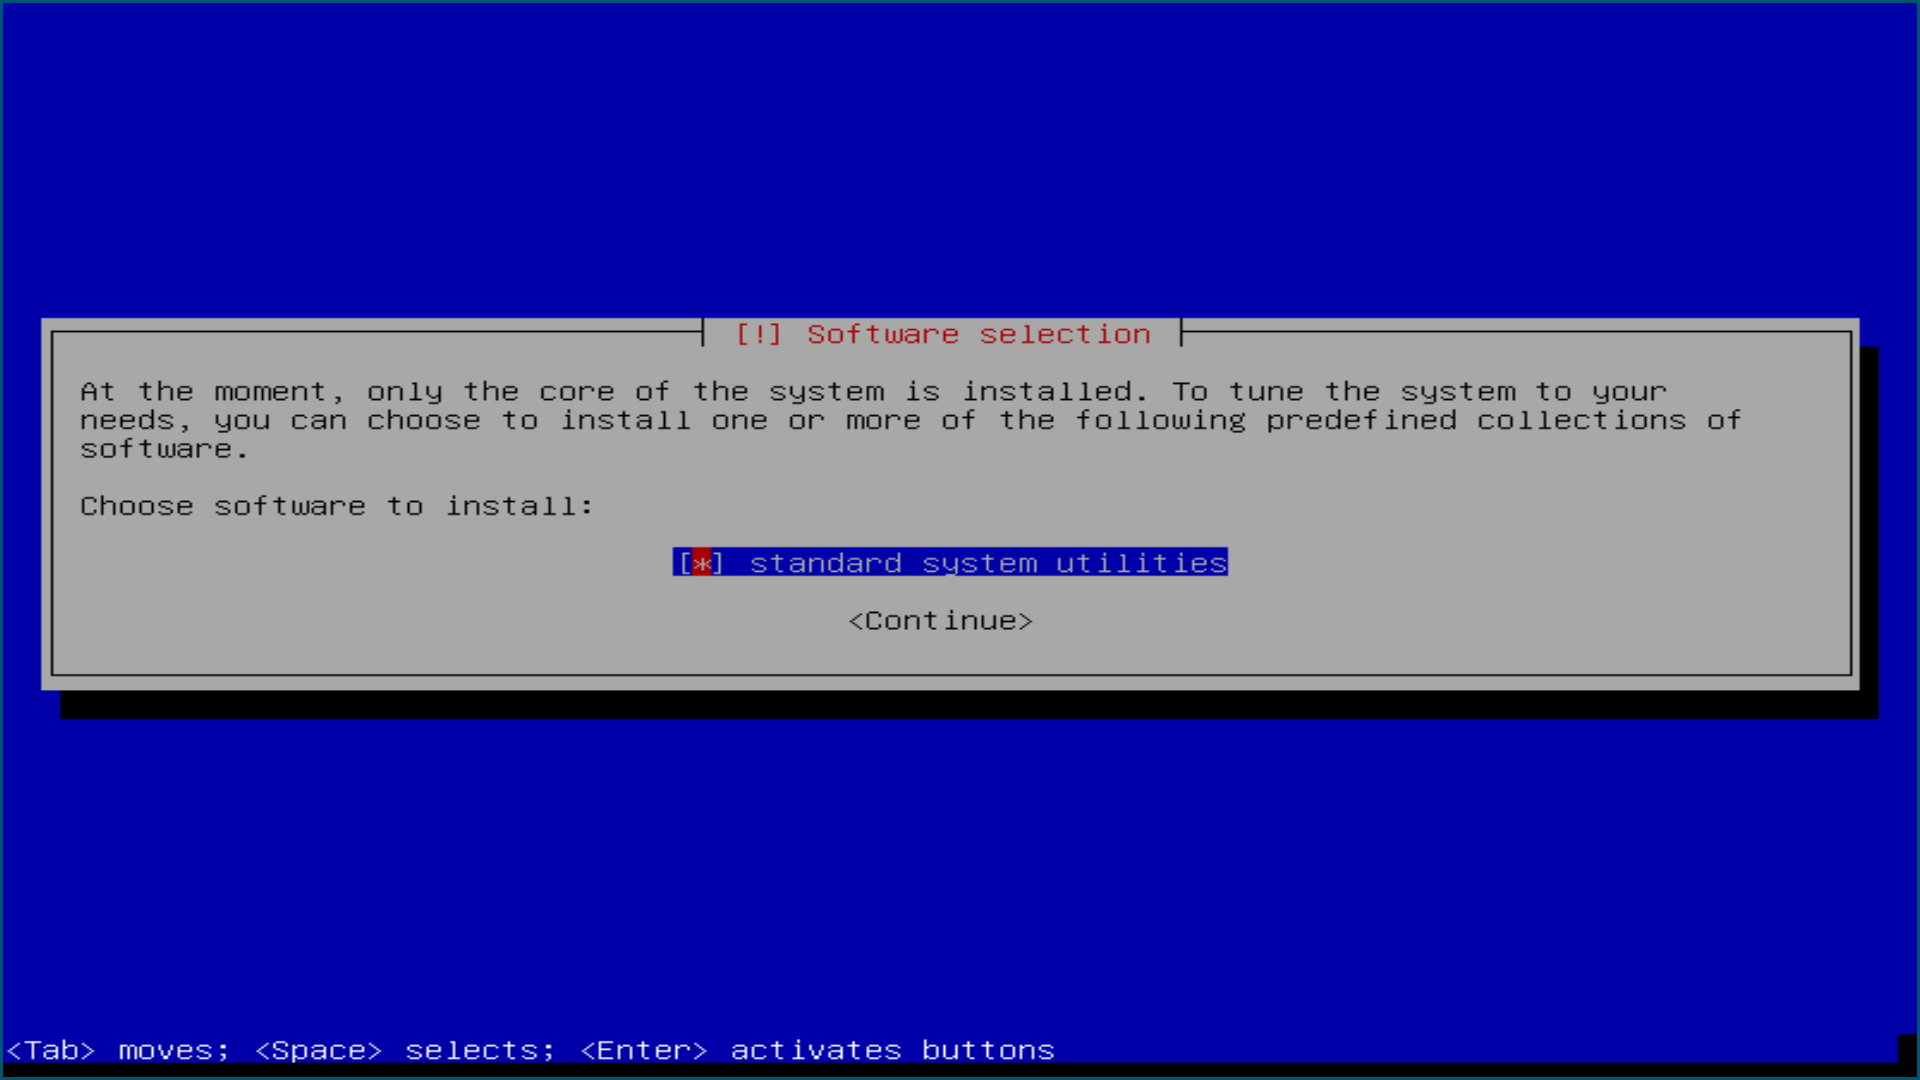
\includegraphics[width=.5\linewidth]{screenshots/25.png}
\caption{就一条,选中它就好。如果你联网了,这里就不止有一条可选了,但也不要选别的,无论如何,就选这一条。}
\end{figure}

\begin{figure}[htbp]
\centering
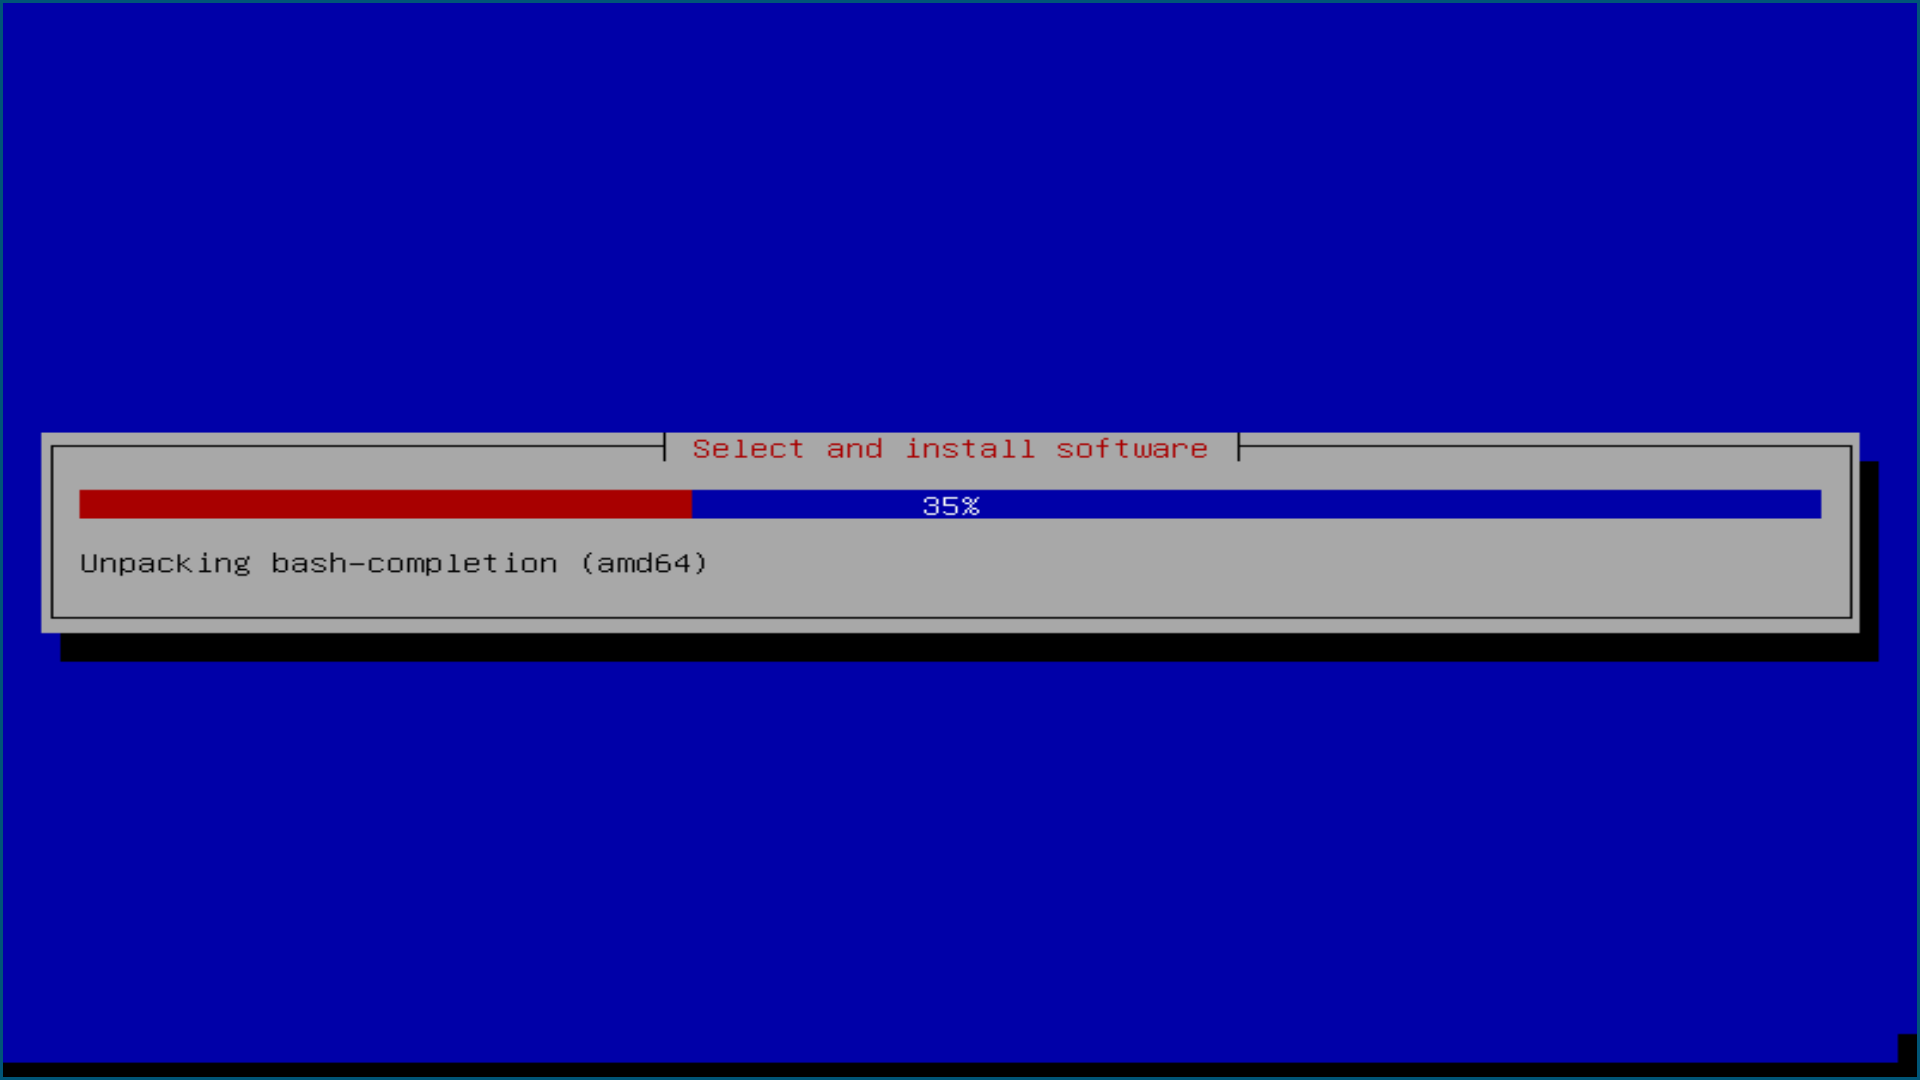
\includegraphics[width=.5\linewidth]{screenshots/26.png}
\caption{大约要10分钟}
\end{figure}

\item 安装GRUB

\begin{figure}[htbp]
\centering
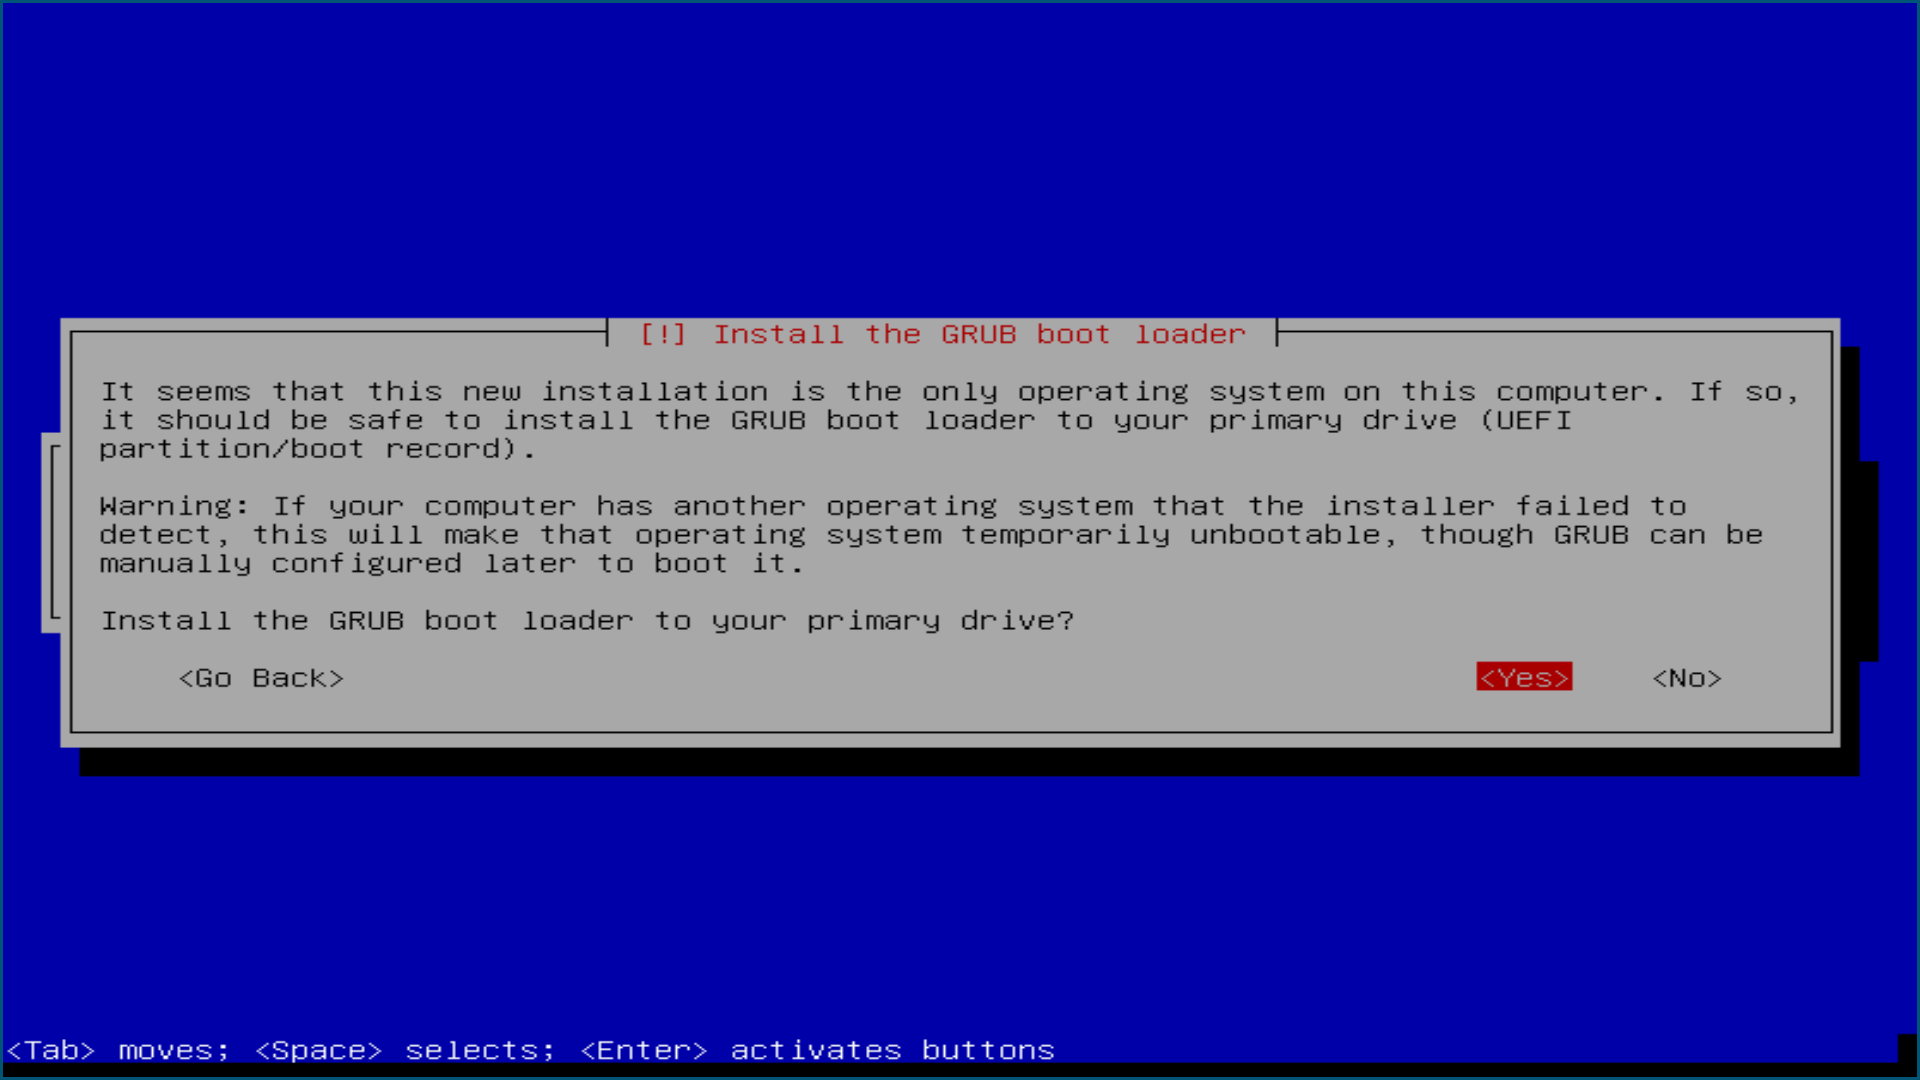
\includegraphics[width=.5\linewidth]{screenshots/27.png}
\caption{选“Yes”}
\end{figure}

\begin{figure}[htbp]
\centering
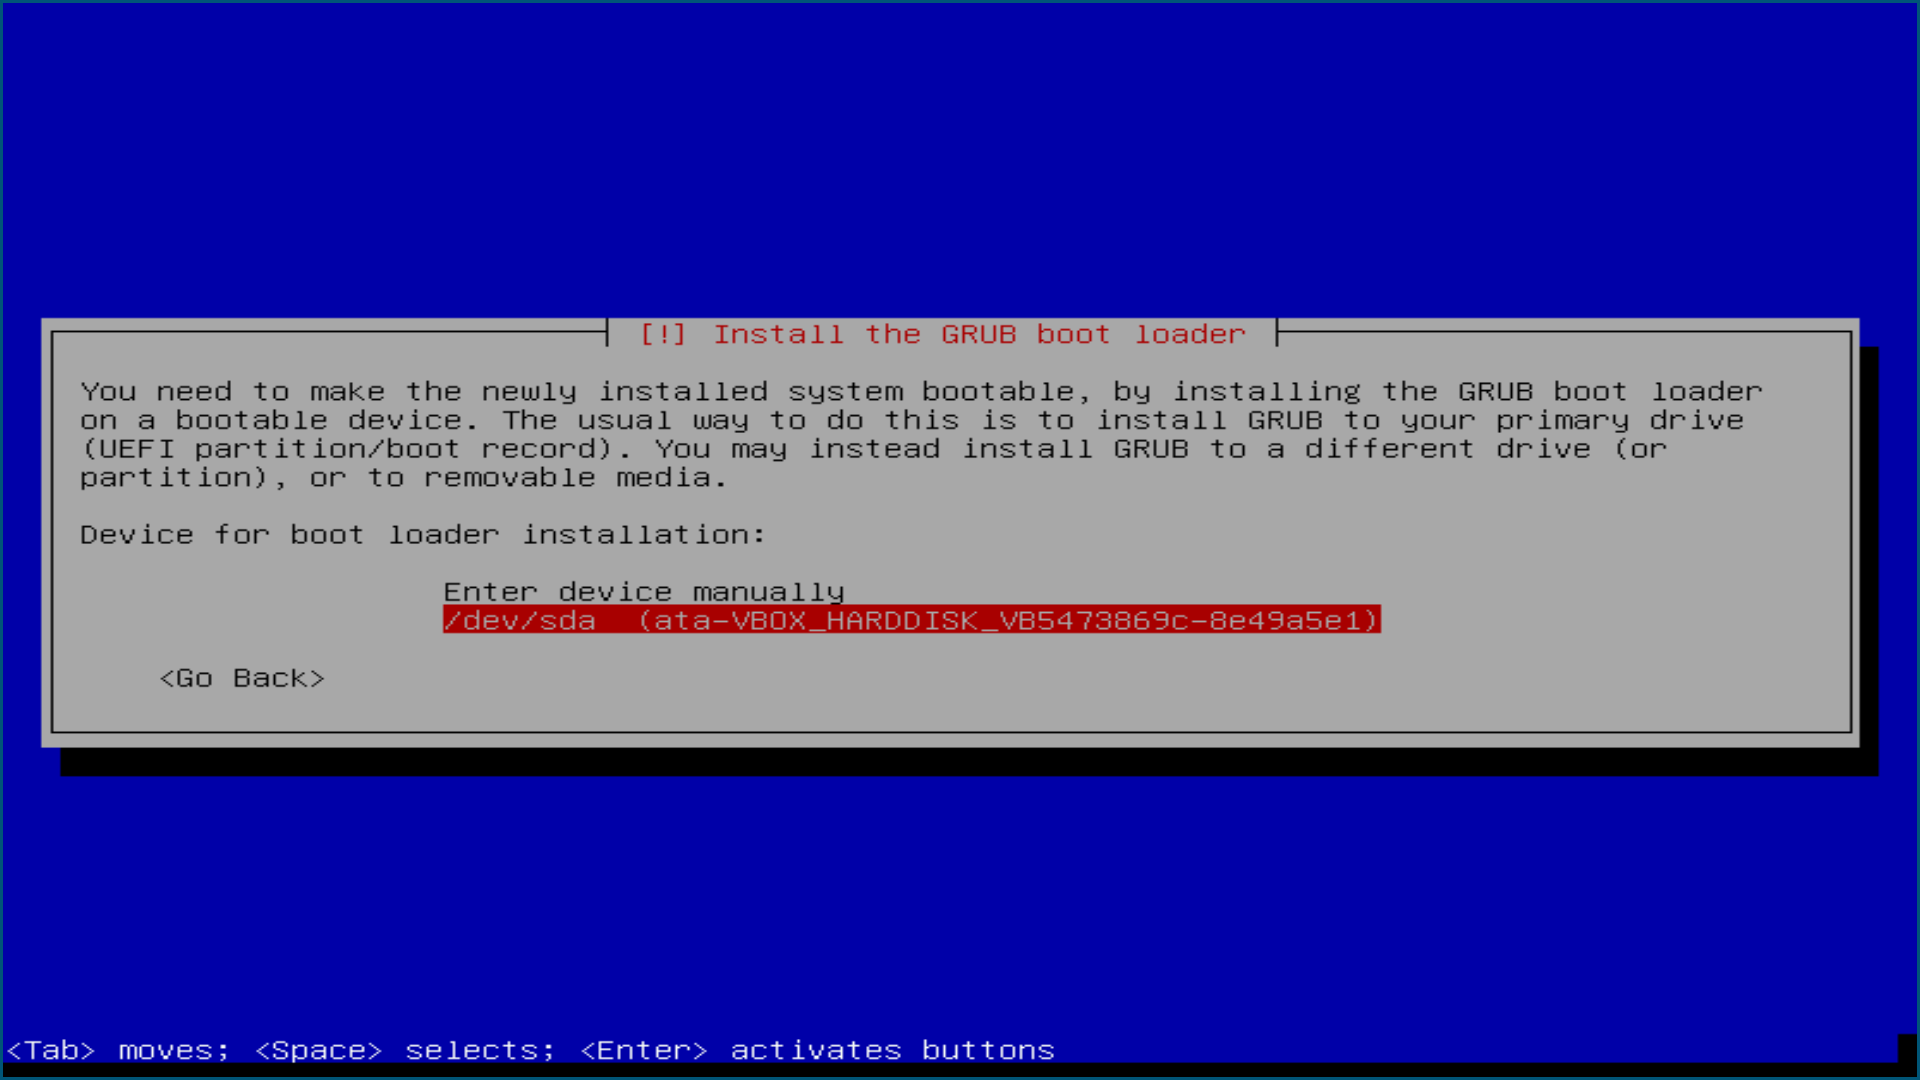
\includegraphics[width=.5\linewidth]{screenshots/28.png}
\caption{如果你有不止一块硬盘,或者不止一个分区,你就要好好斟酌了,千万别装错了地方。}
\end{figure}

\item 安装结束

\begin{center}
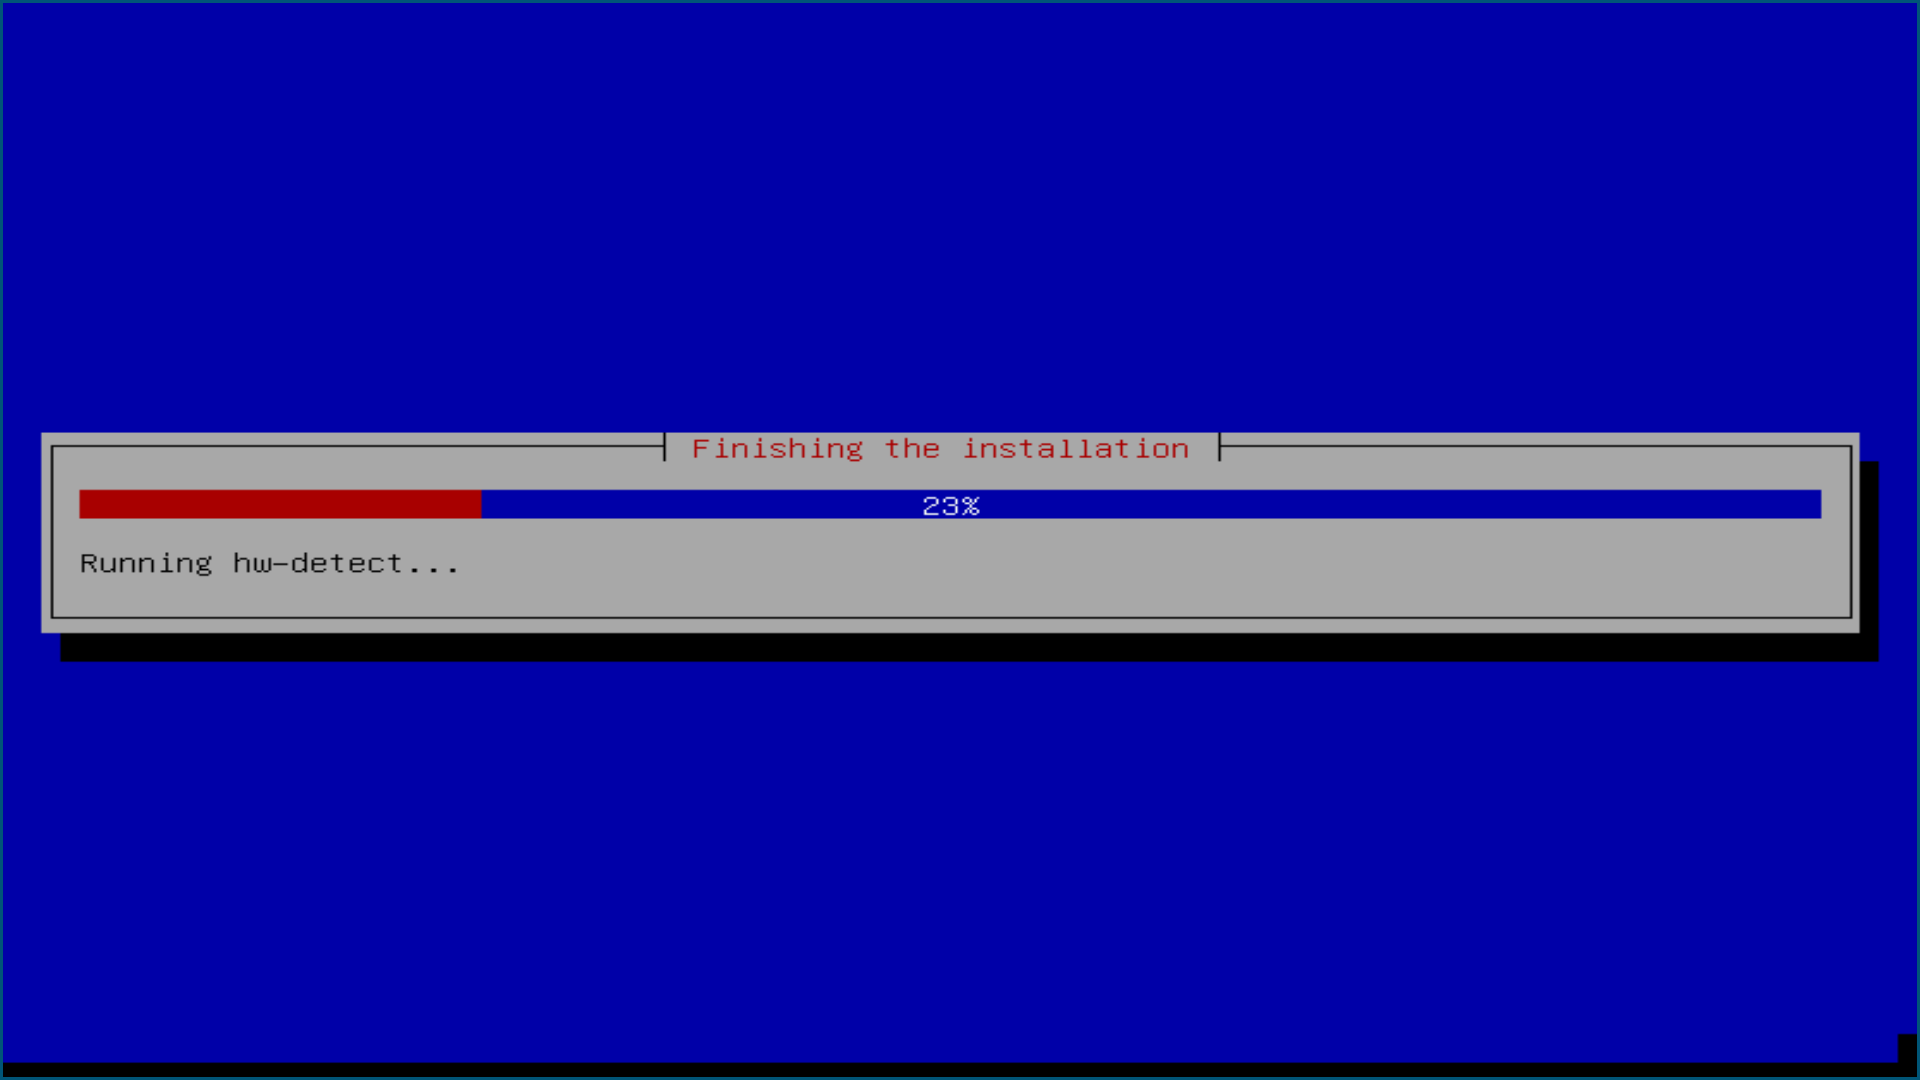
\includegraphics[width=.5\linewidth]{screenshots/29.png}
\end{center}

\begin{figure}[htbp]
\centering
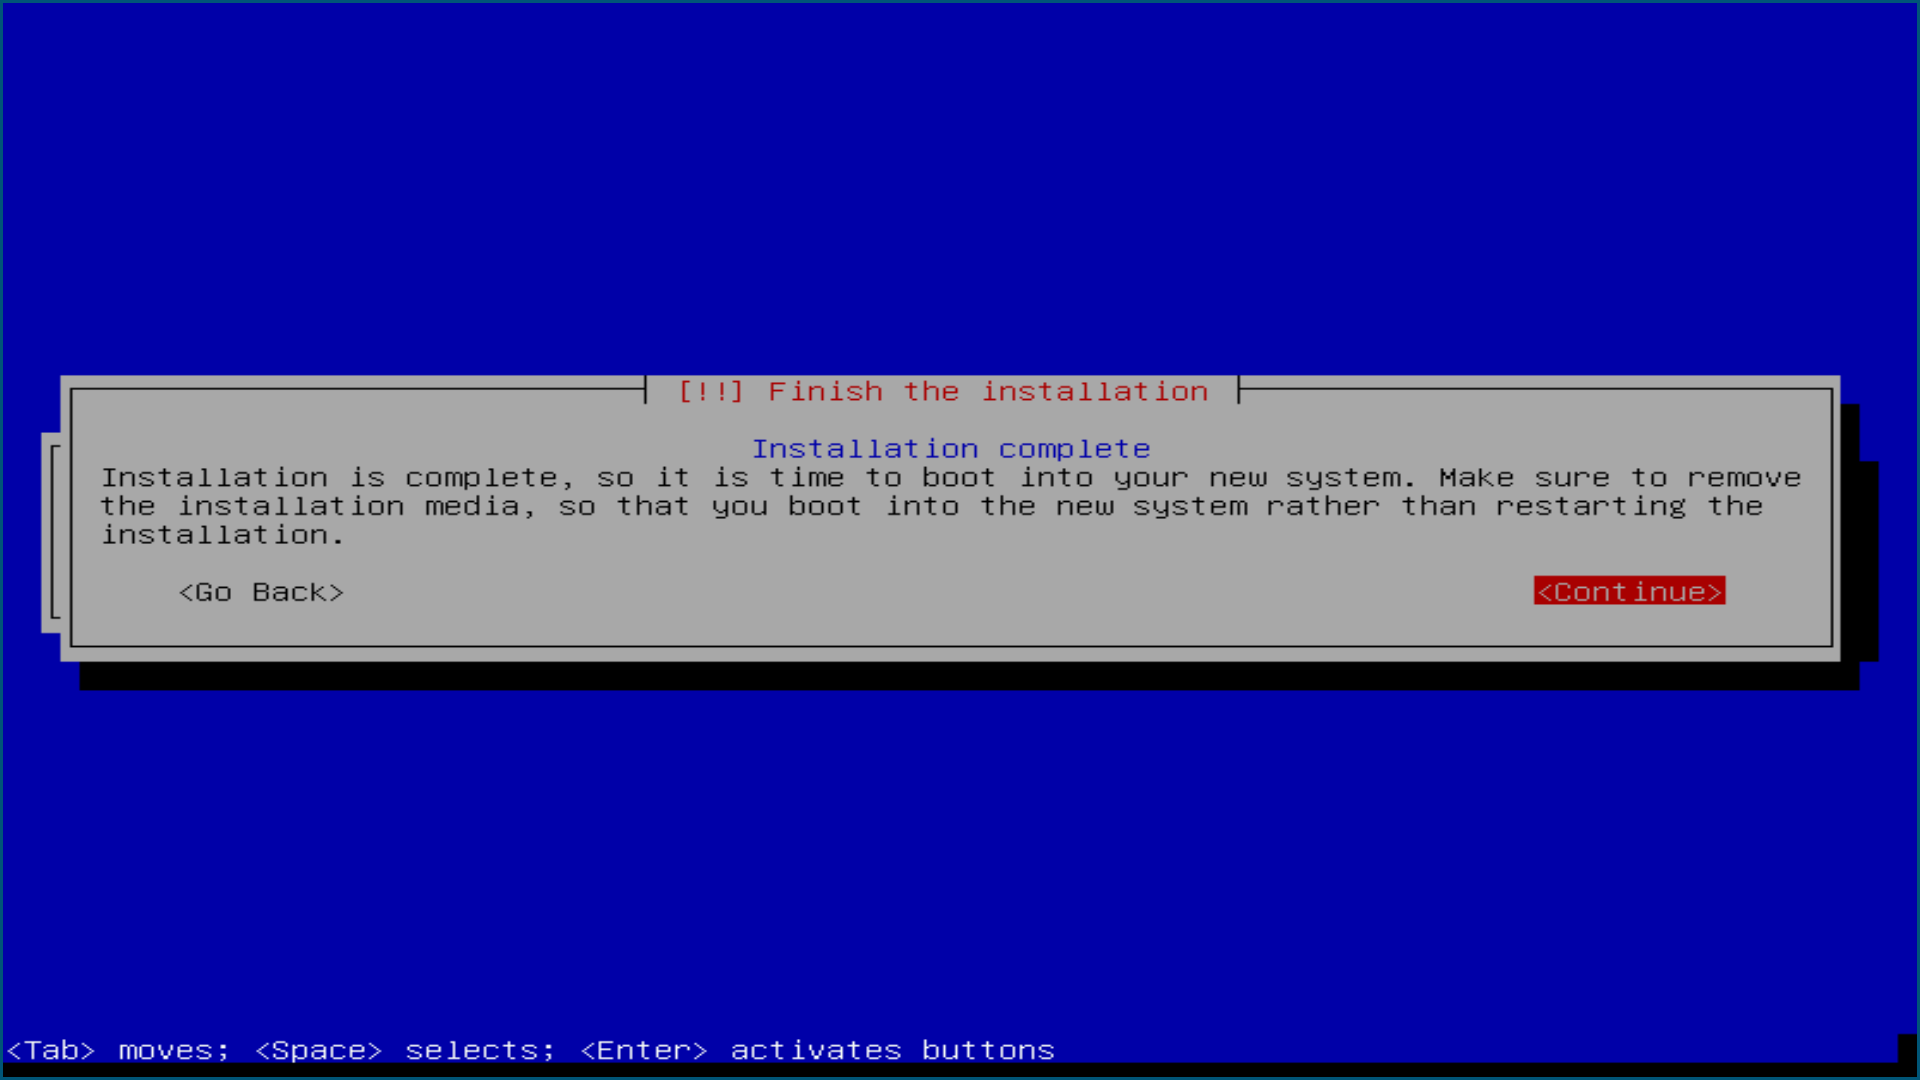
\includegraphics[width=.5\linewidth]{screenshots/30.png}
\caption{拔掉U盘,回车,电脑重启}
\end{figure}

\begin{figure}[htbp]
\centering
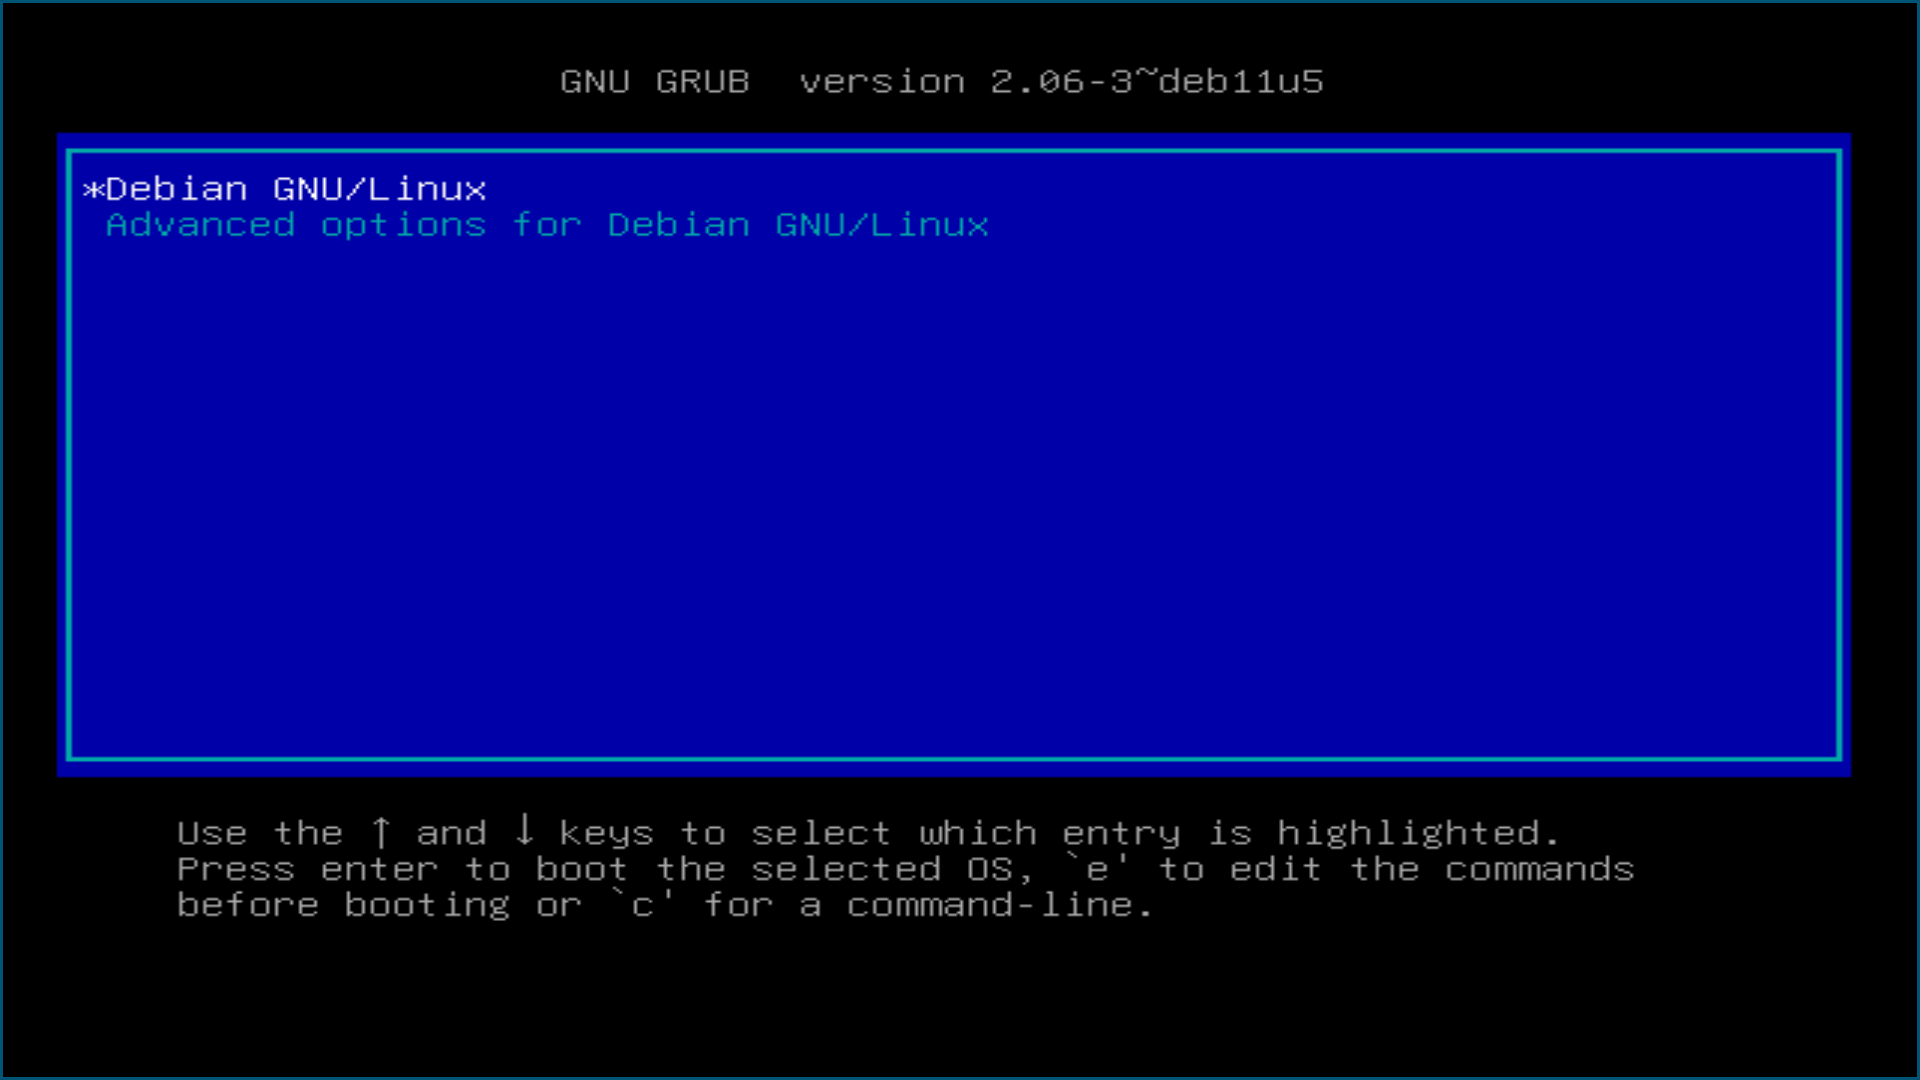
\includegraphics[width=.5\linewidth]{screenshots/31.png}
\caption{重启之后,应该是这个样子。如果是双系统的话,你还应该能看到一条关于Windows的选项。}
\end{figure}
\end{enumerate}

\section{安装完整系统}
\label{sec:org72fcbfc}

好消息!现在,你只要下载并运行\href{https://cs6.swfu.edu.cn/\~wx672/debian-install/install.sh}{这个小程序},就可以得到一个完整的Debian系统了。
\begin{enumerate}
\item 登录

\begin{center}
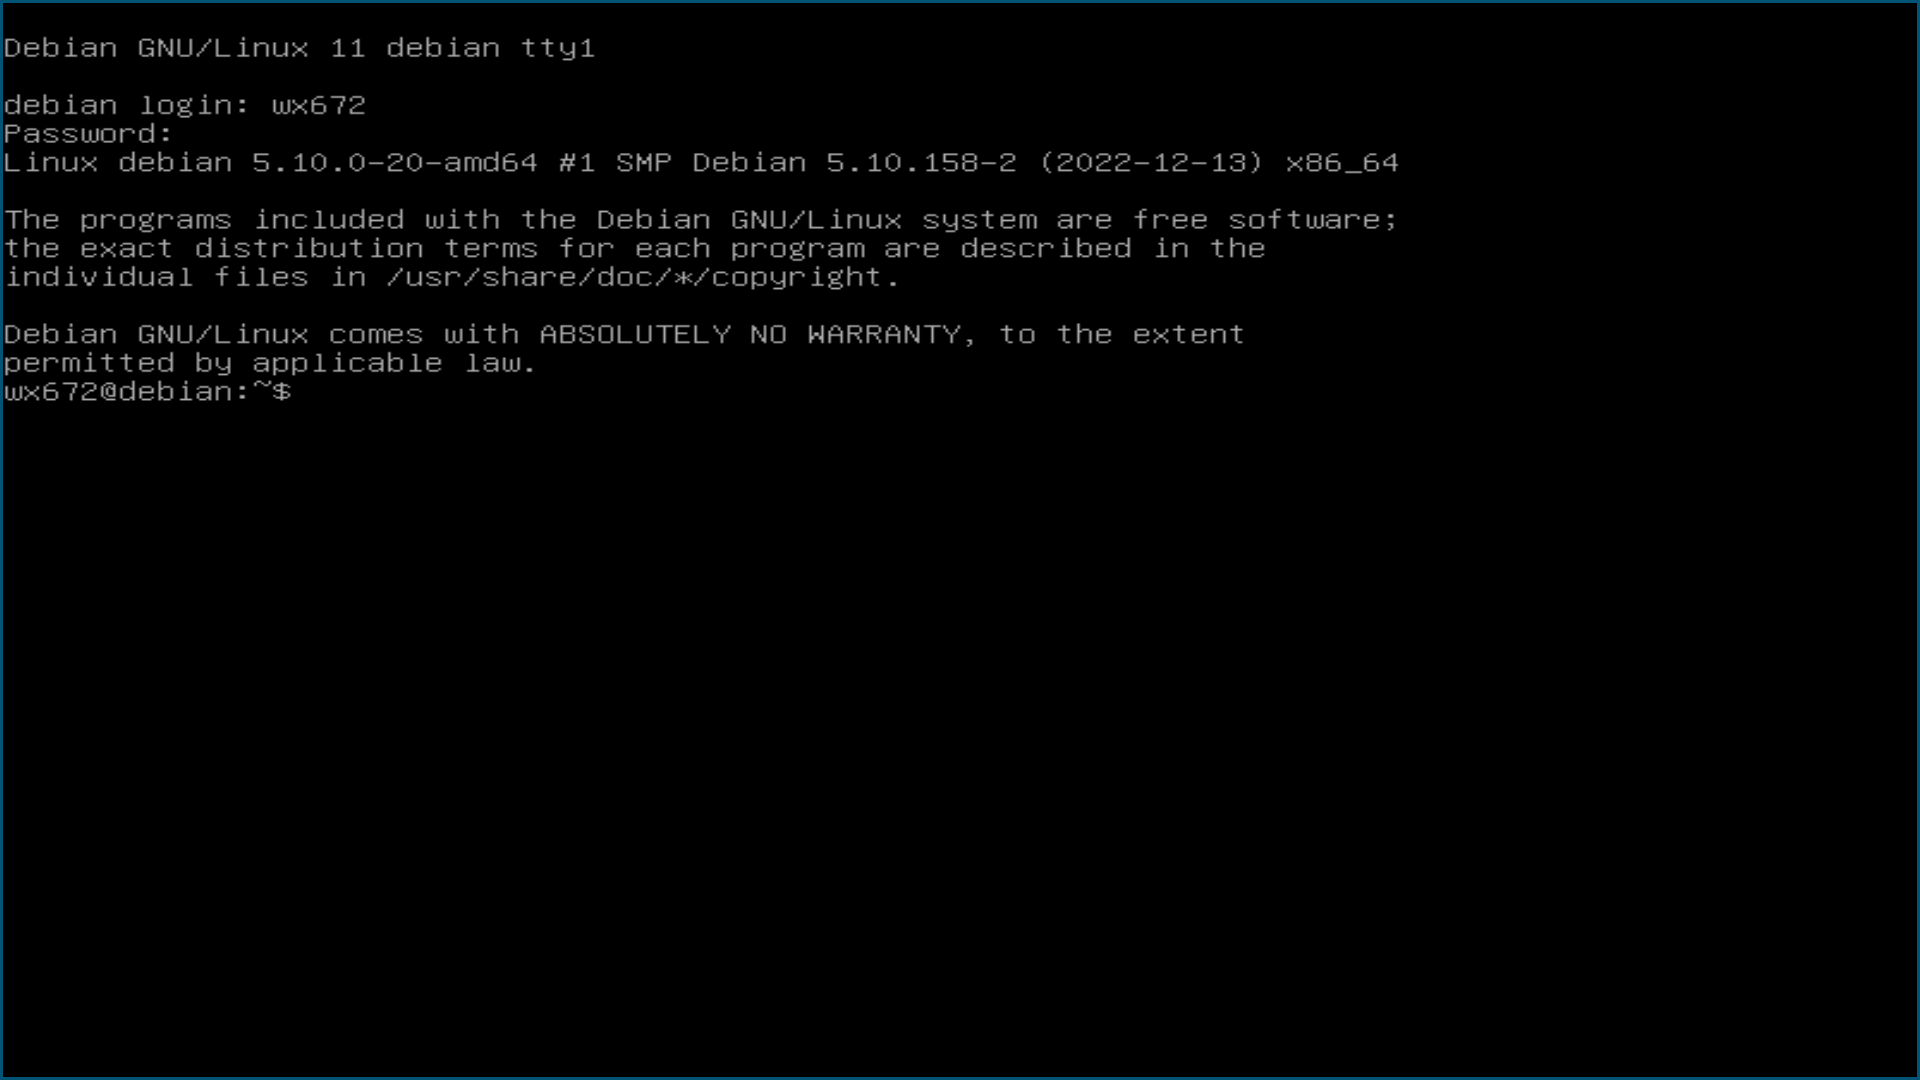
\includegraphics[width=.5\linewidth]{screenshots/33.png}
\end{center}

\item 联网。当然要先插好网线。如果你的笔记本比较新潮,没有有线网口,那么可以试试下面两个办法:
\begin{itemize}
\item 你可以利用手机的 Ethernet tethering 功能,详见第\ref{sec:orgd858525}节。
\item 找一个USB-Ethernet转接头。十几块钱就能买一个。
\end{itemize}

总之,现在刚装完最小系统,无线网很可能还不好使。连好网线,再敲下面的命令,应该就能连上网了。

\begin{minted}[mathescape=true,linenos=true,numbersep=5pt,frame=lines,framesep=2mm]{sh}
ip a          #注释:查看网卡是否已经有IP地址了
sudo dhclient #注释:自动获得IP地址
\end{minted}

\begin{figure}[htbp]
\centering
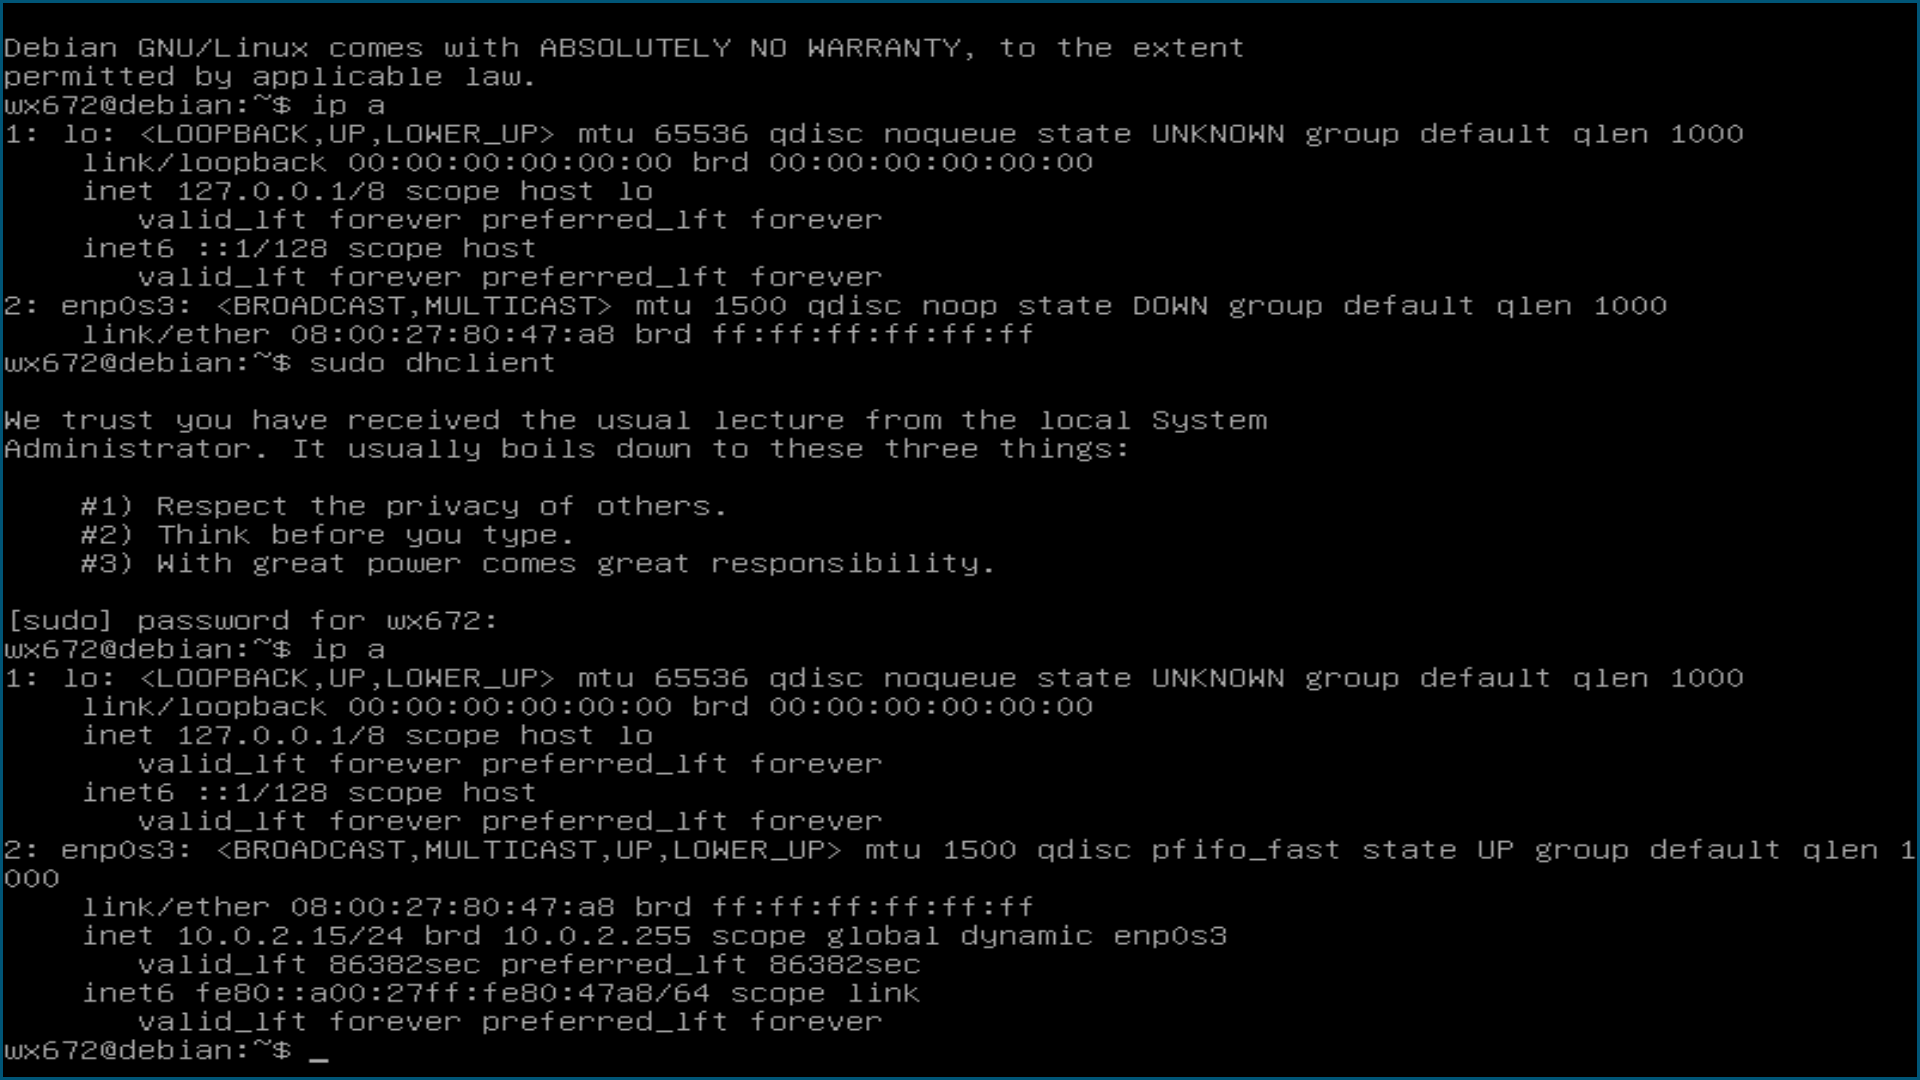
\includegraphics[width=.5\linewidth]{screenshots/36.png}
\caption{敲命令联网的全过程}
\end{figure}

\item 下载

\begin{minted}[mathescape=true,linenos=true,numbersep=5pt,frame=lines,framesep=2mm]{sh}
cd
wget cs6.swfu.edu.cn/~wx672/debian-install/install.sh
\end{minted}

\begin{figure}[htbp]
\centering
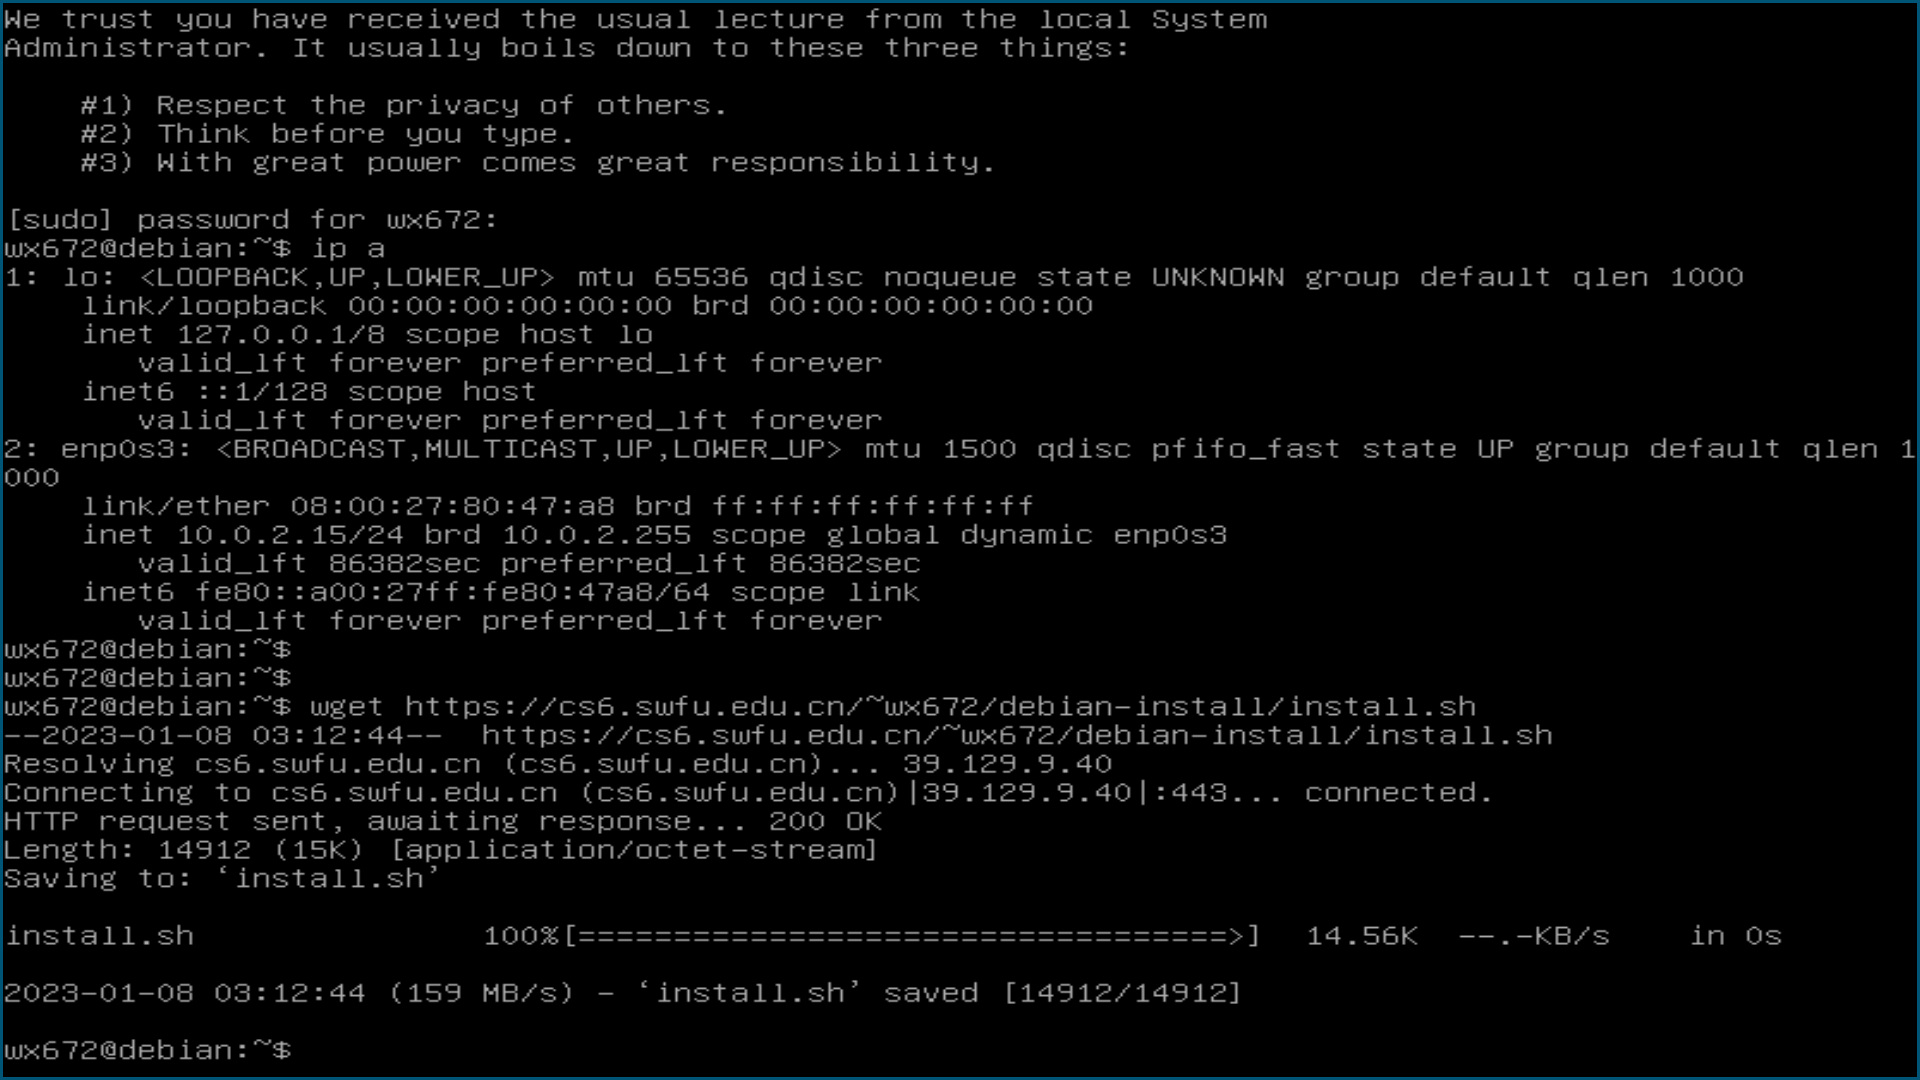
\includegraphics[width=.5\linewidth]{screenshots/37.png}
\caption{用 \texttt{wget} 下载安装程序(\textasciitilde{}install.sh\textasciitilde{})}
\end{figure}

\item 运行

\begin{minted}[mathescape=true,linenos=true,numbersep=5pt,frame=lines,framesep=2mm]{sh}
chmod +x install.sh
./install.sh
\end{minted}

\begin{figure}[htbp]
\centering
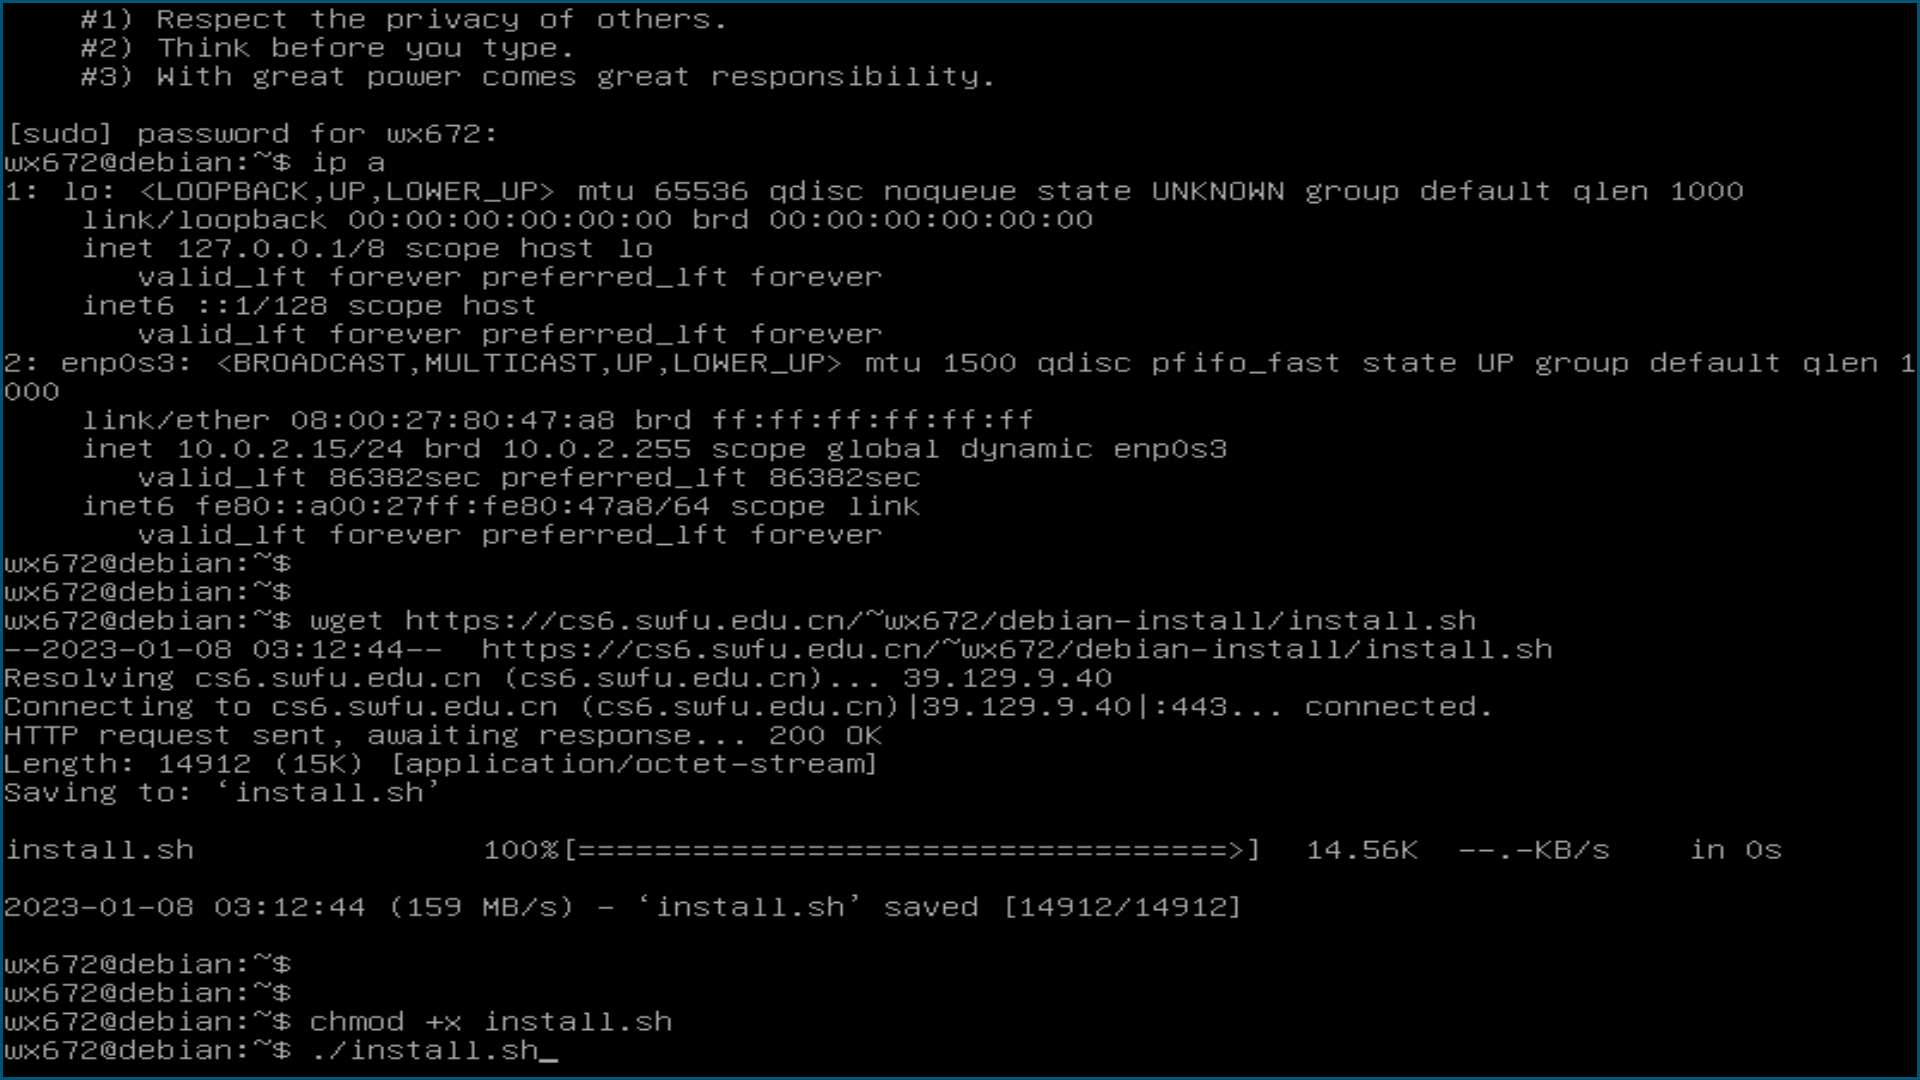
\includegraphics[width=.5\linewidth]{screenshots/38.png}
\caption{开始安装}
\end{figure}

网络顺畅的话,半个小时应该就完事了。不顺畅的话……把网络搞顺畅了再说吧。

\textbf{程序运行过程中,会不时给出英文提示,千万要耐心看明白,然后再操作。}

\textbf{不要忽略任何一个提示!不要忽略提示!不要忽略提示!}

\begin{figure}[htbp]
\centering
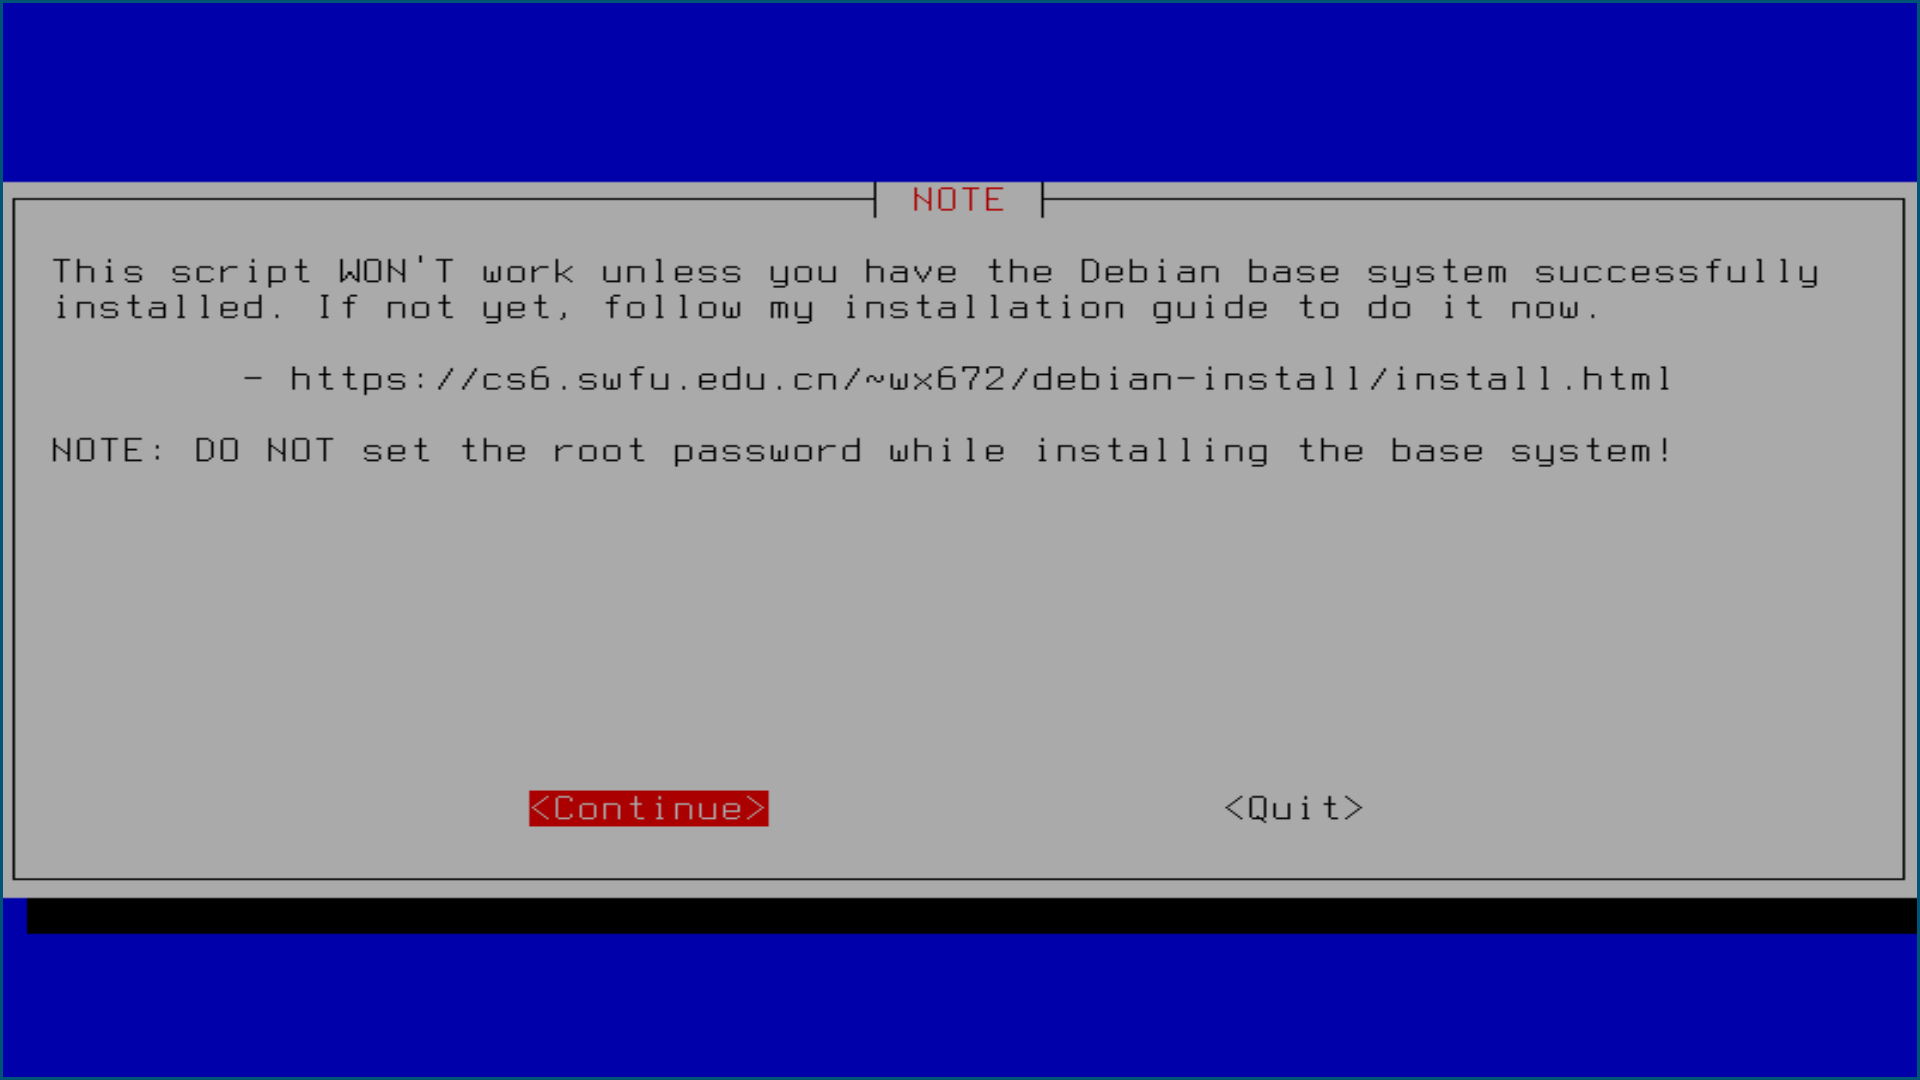
\includegraphics[width=.5\linewidth]{screenshots/39.png}
\caption{当然选择“Continue”}
\end{figure}

\begin{figure}[htbp]
\centering
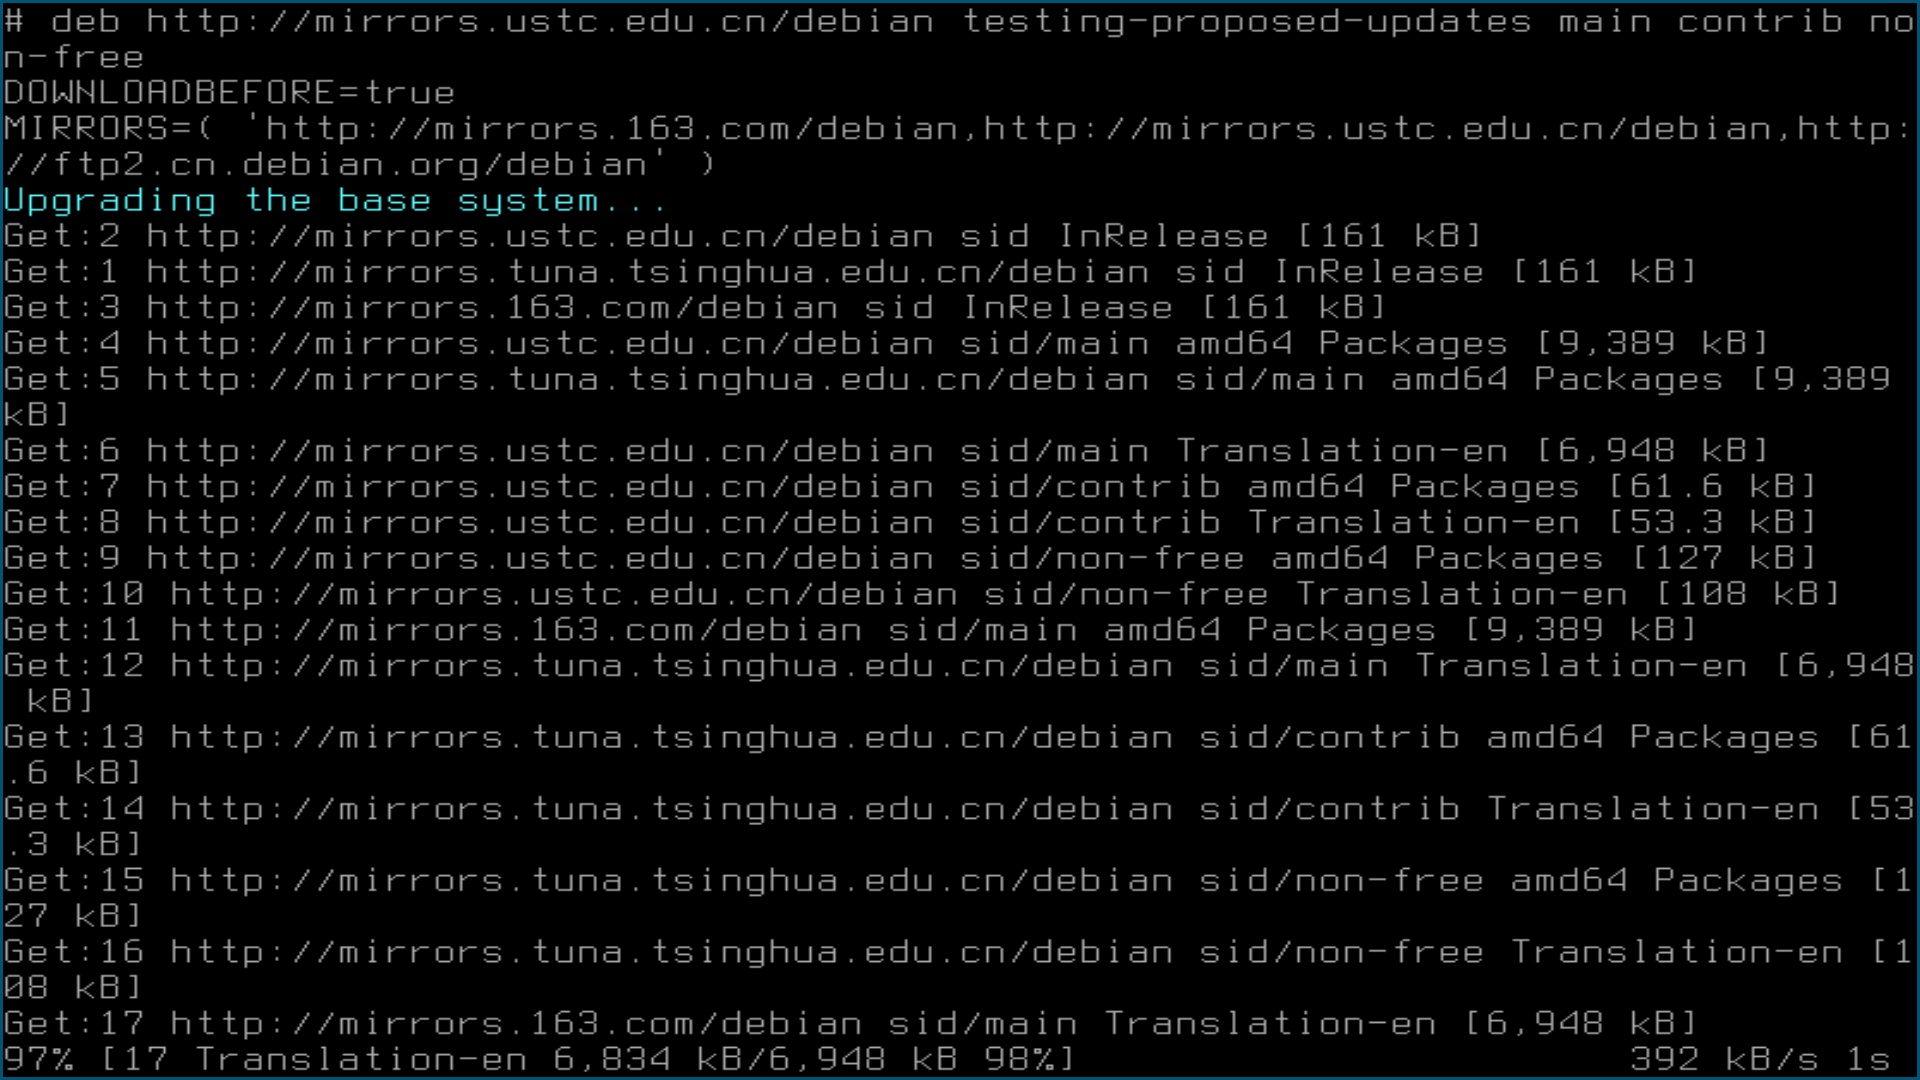
\includegraphics[width=.5\linewidth]{screenshots/40.png}
\caption{升级最小系统。网络没问题的话,这一步不会出毛病,10分钟就能结束。}
\end{figure}

\begin{figure}[htbp]
\centering
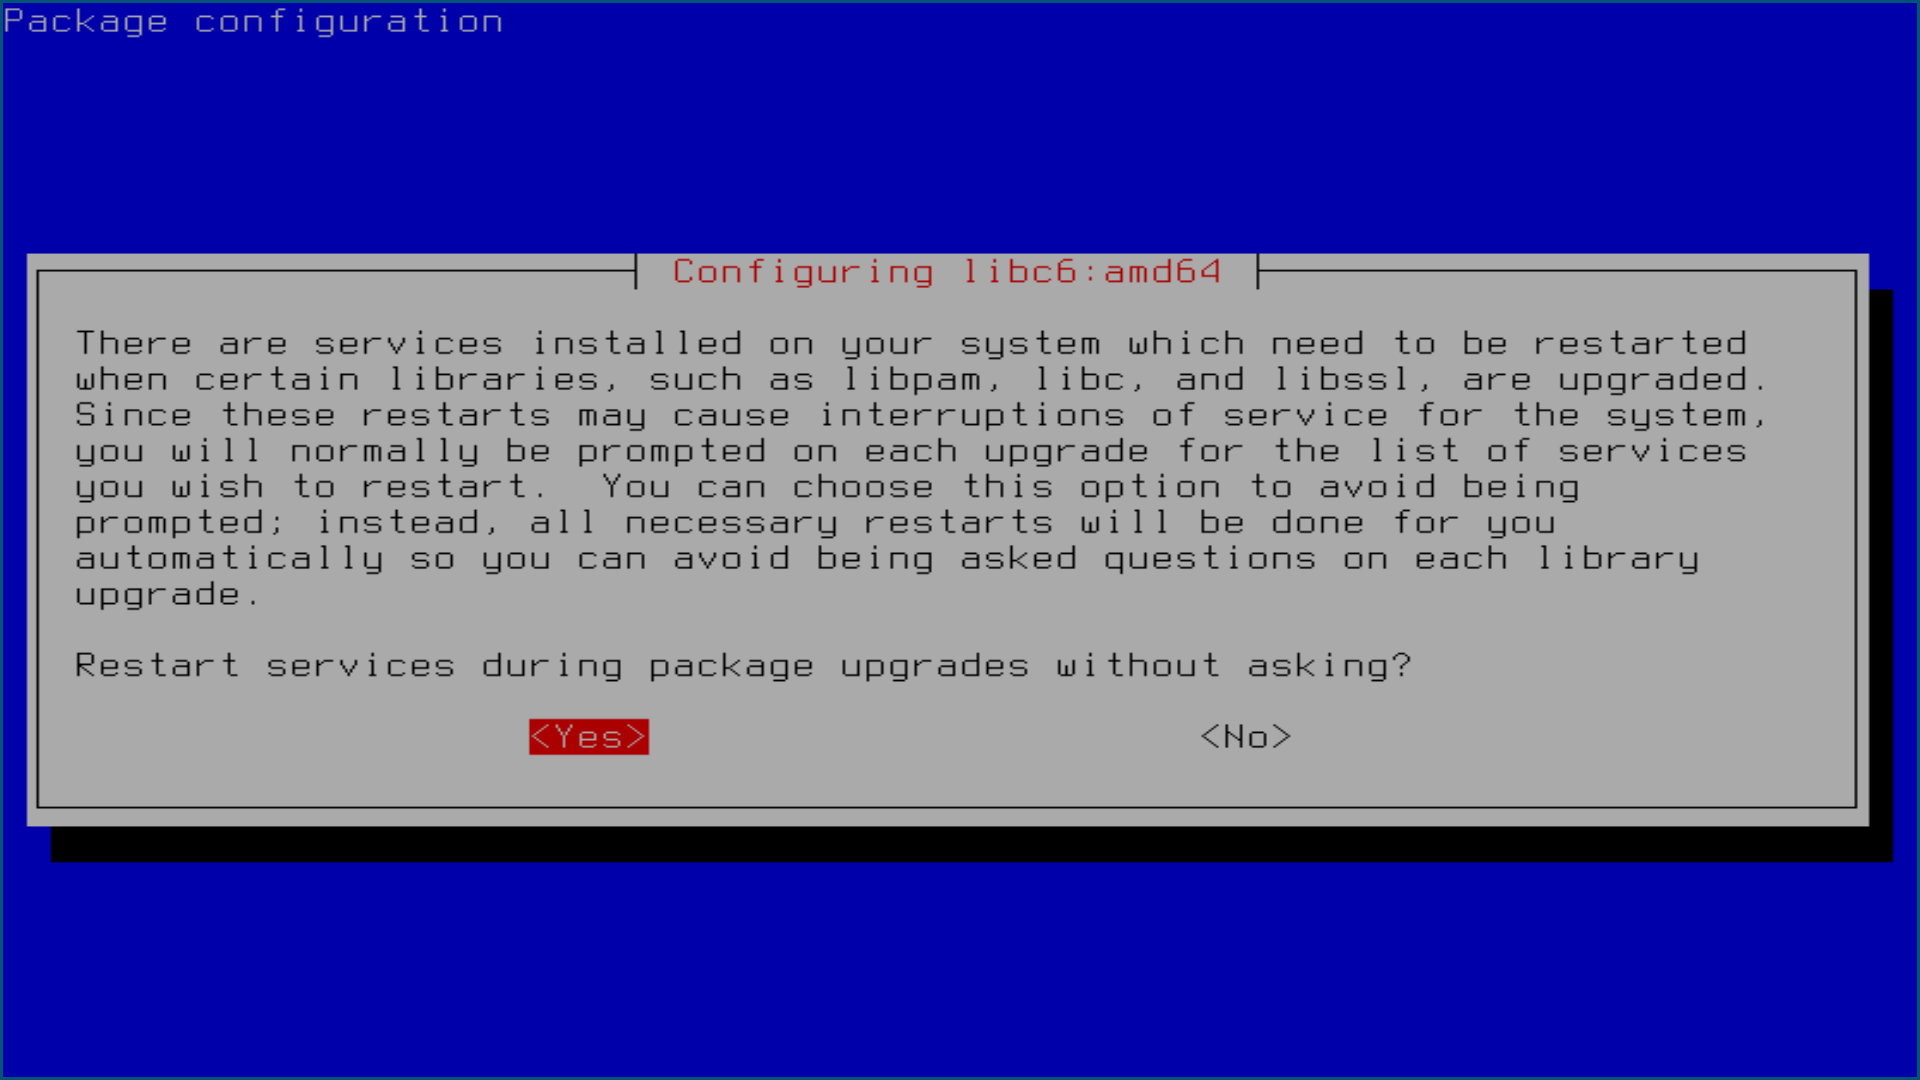
\includegraphics[width=.5\linewidth]{screenshots/41.png}
\caption{选“Yes”}
\end{figure}

\begin{figure}[htbp]
\centering
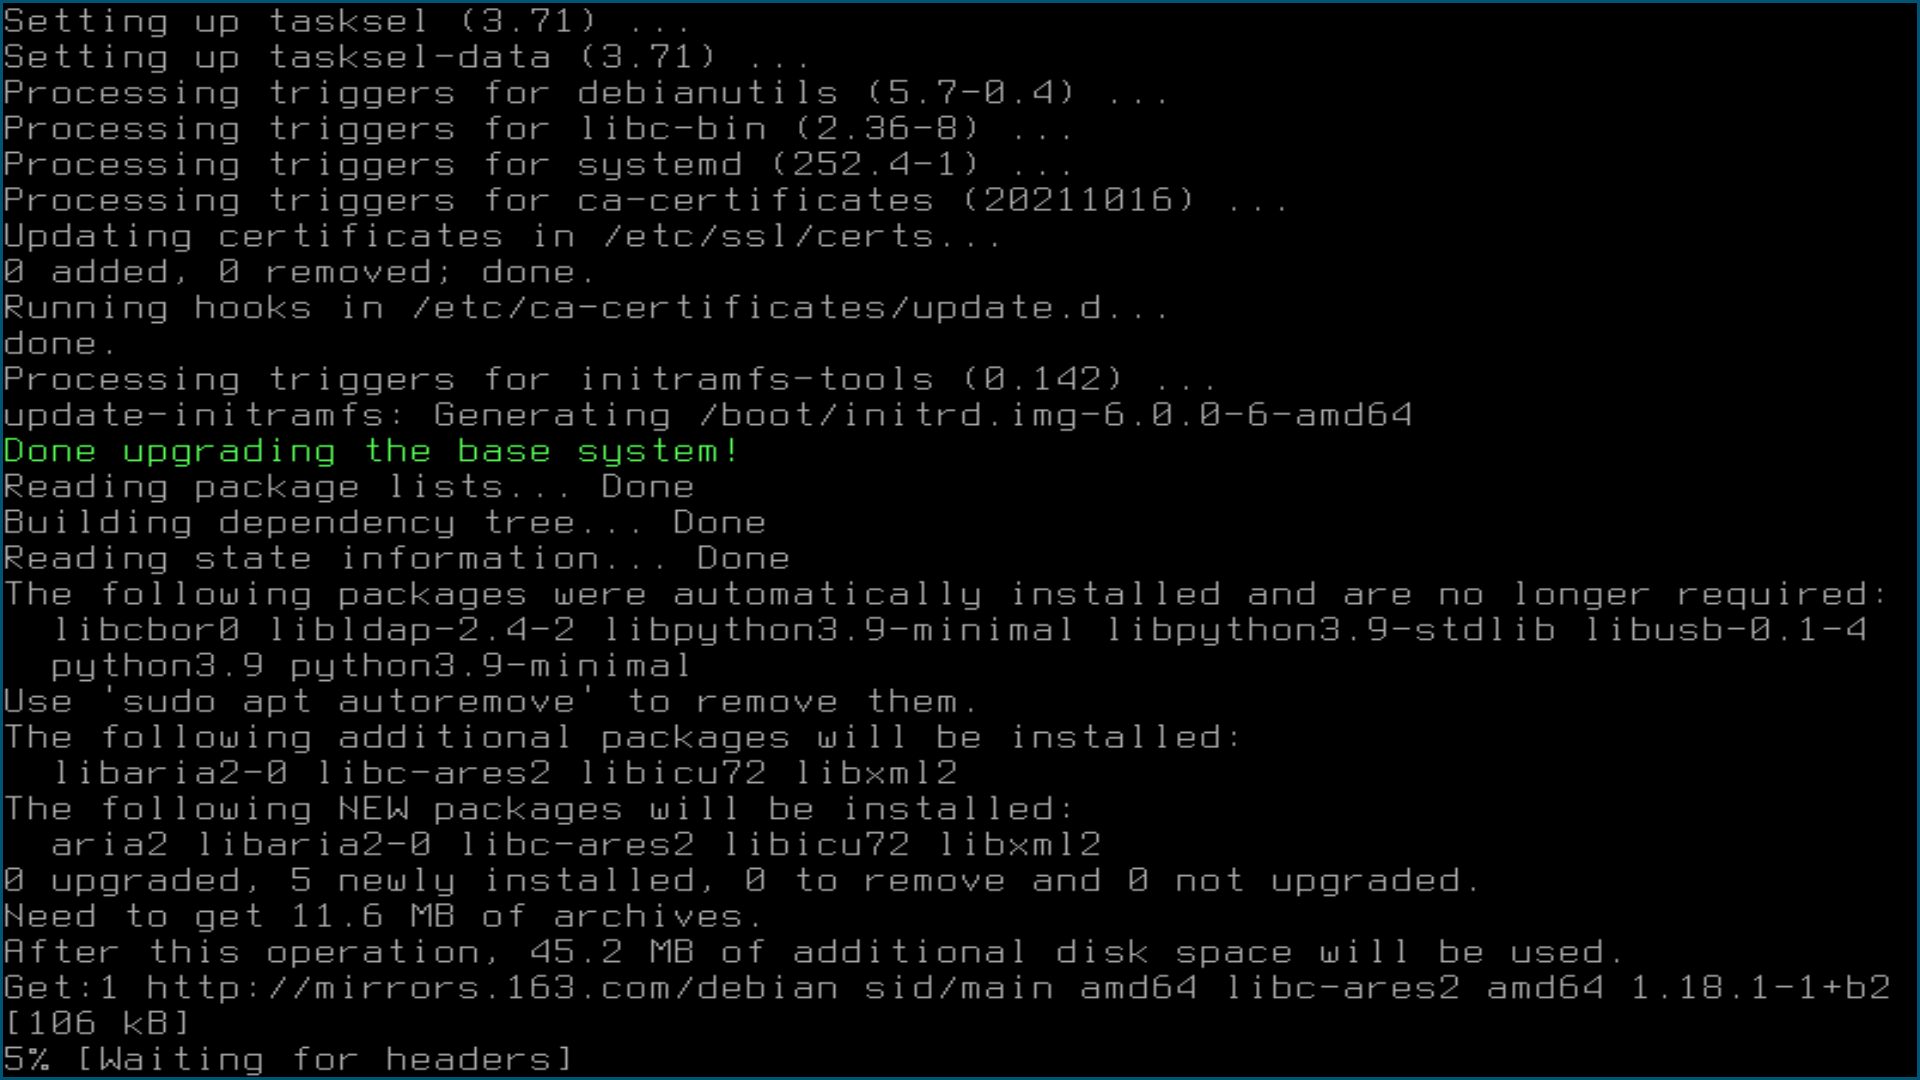
\includegraphics[width=.5\linewidth]{screenshots/43.png}
\caption{最小系统升级顺利结束。白字和绿字都很好,如果看见红字(报错)就要小心了。}
\end{figure}

\begin{figure}[htbp]
\centering
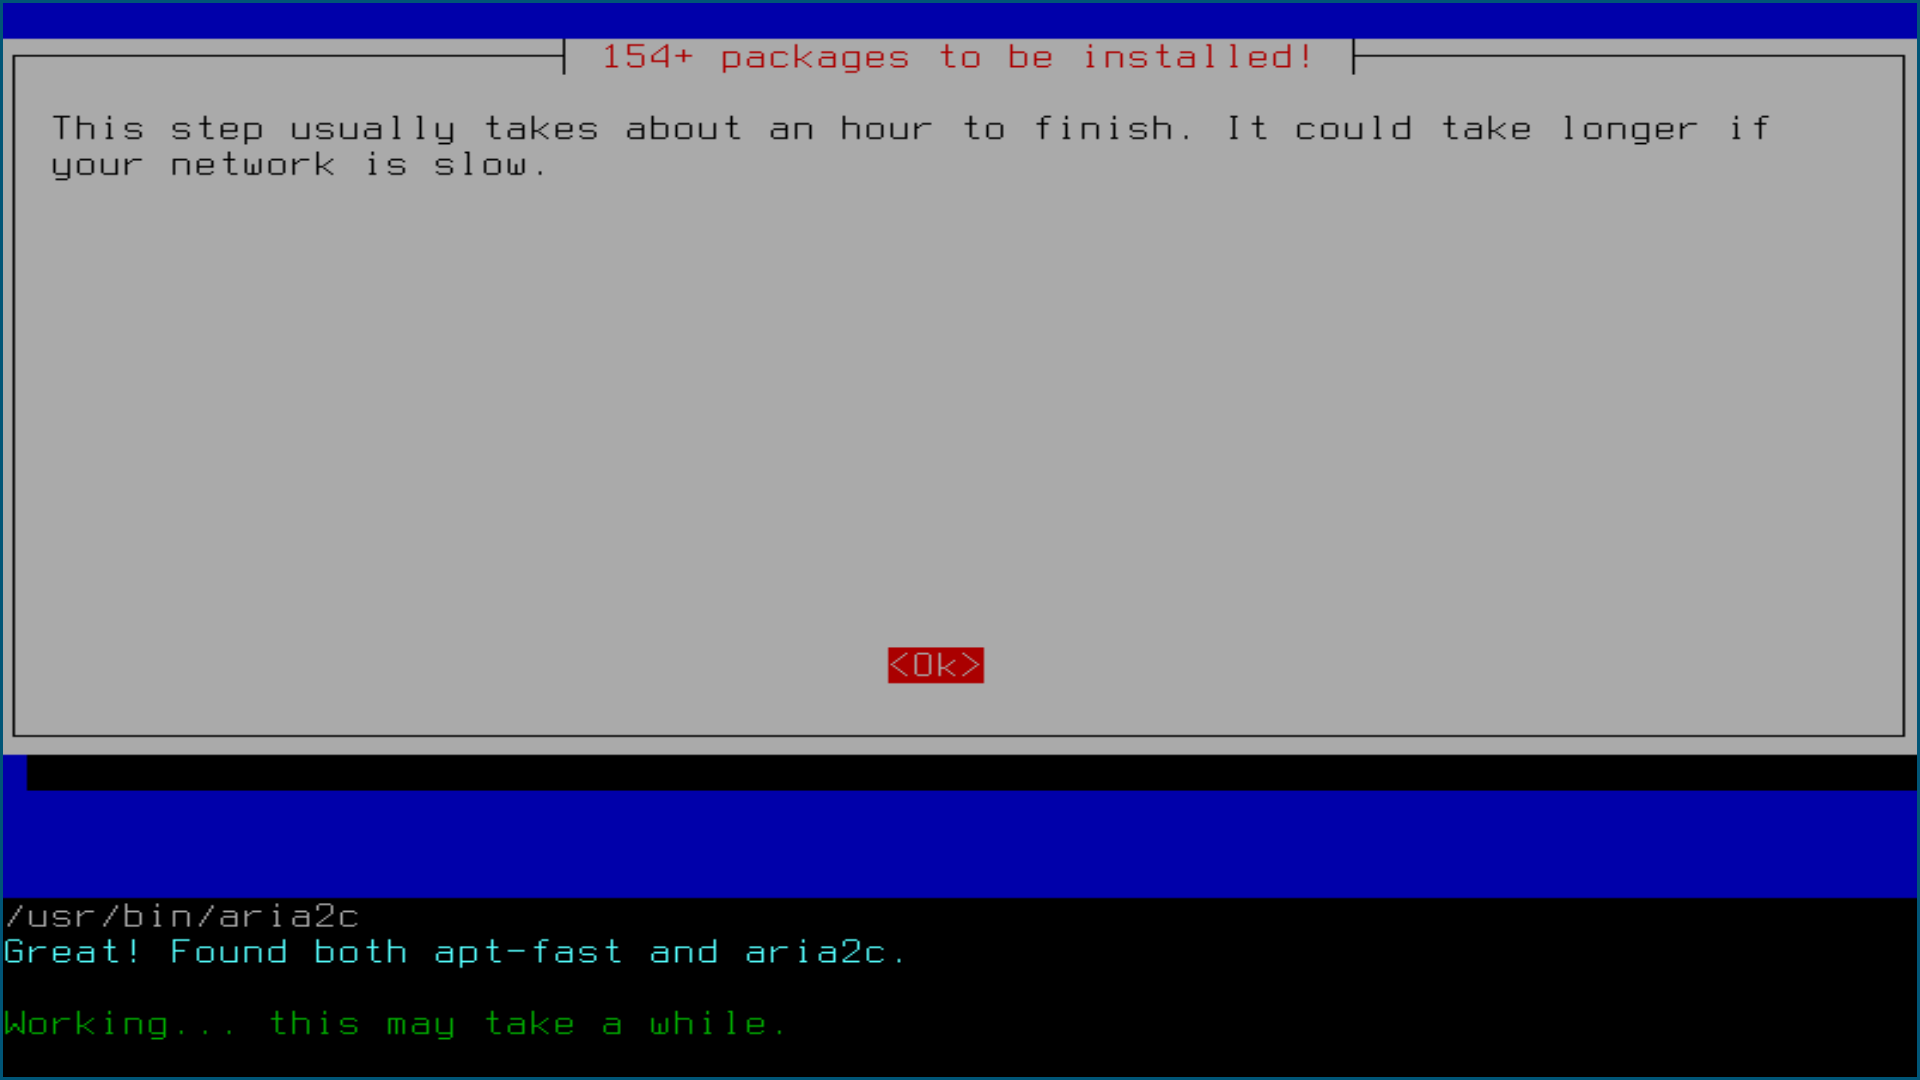
\includegraphics[width=.5\linewidth]{screenshots/44.png}
\caption{正常友善提示,回车继续}
\end{figure}

\begin{figure}[htbp]
\centering
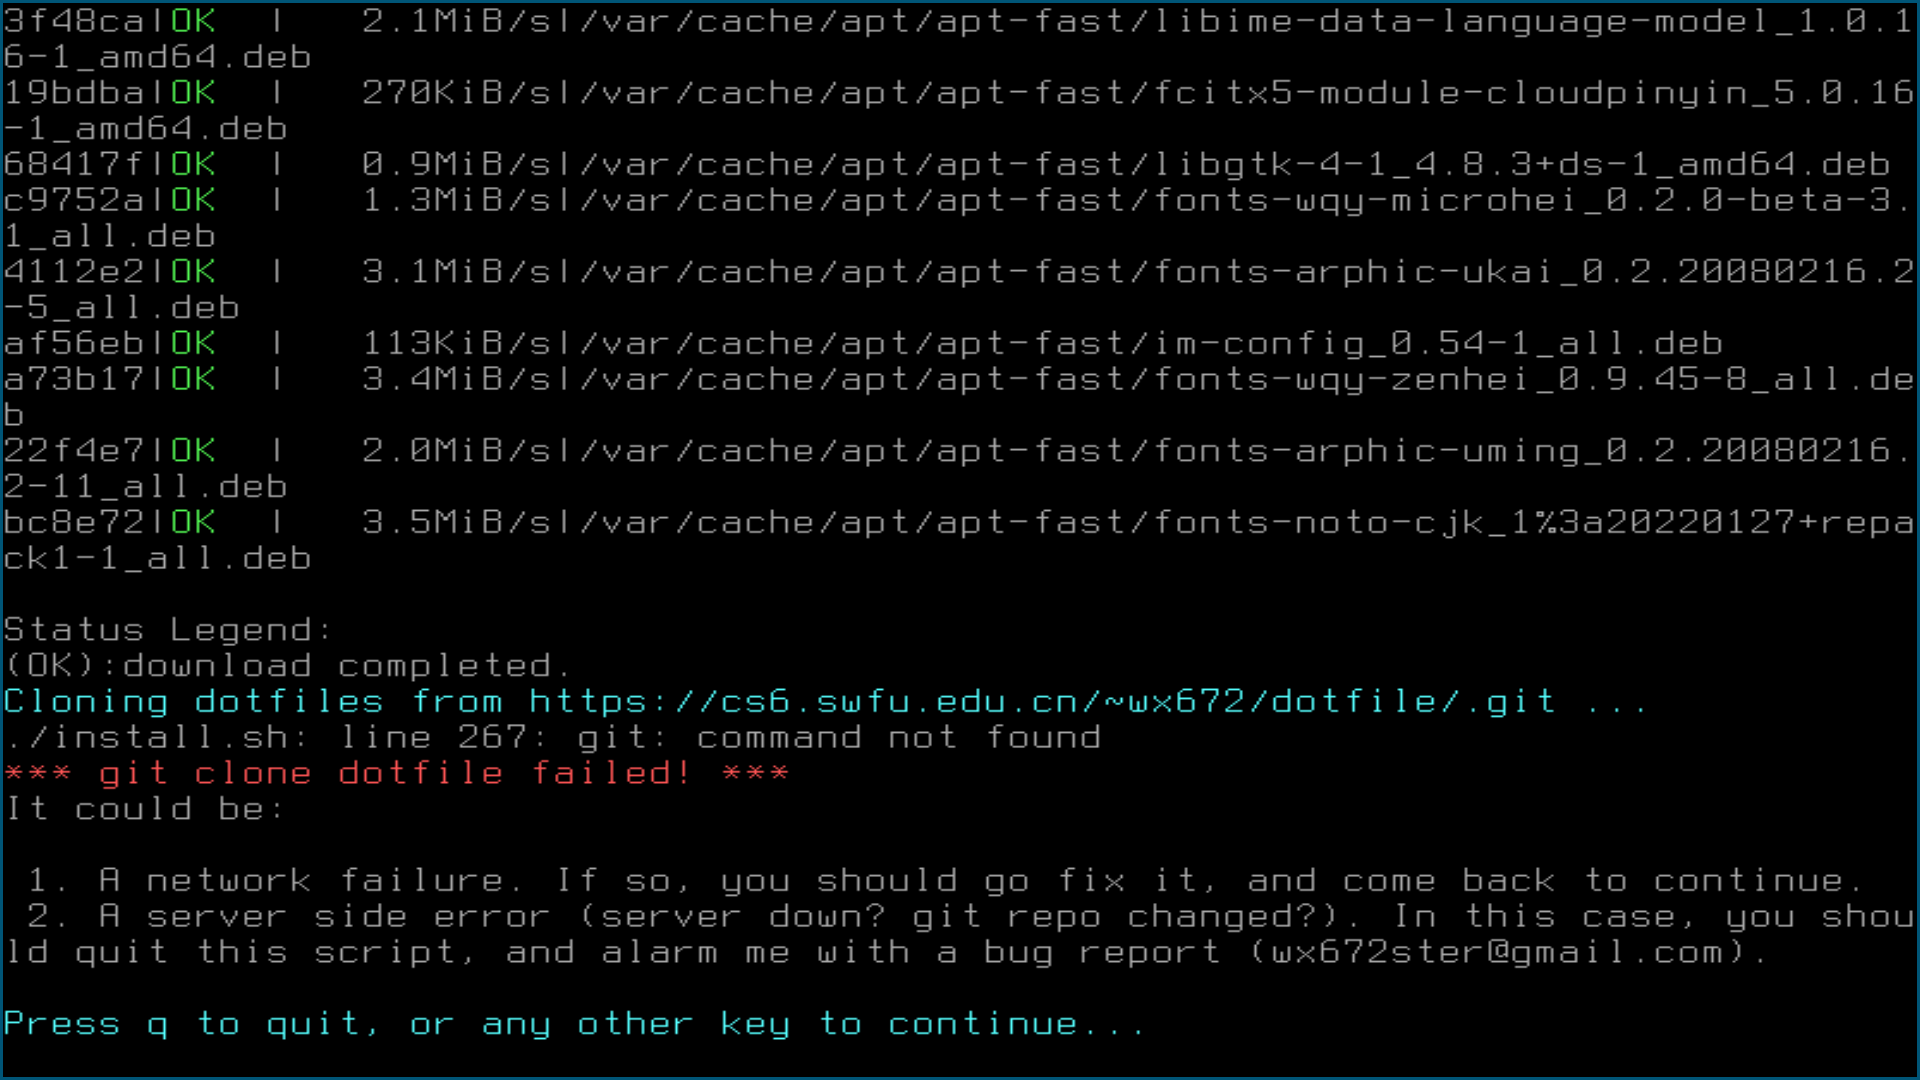
\includegraphics[width=.5\linewidth]{screenshots/45.png}
\caption{出错了!别紧张,下面我就来详细说说遇到问题该怎么办。}
\end{figure}

首先要看明白具体的出错信息。“ \texttt{git: command not found} ”,我估计初学
者不容易看明白发生了什么。 \texttt{git} 是我们在安装过程中要用到的一个命令,
居然没找到,怎么办?其实,我也感觉很意外,前面一切都很顺利,没看见
红字啊。初步判断,是我这个安装程序( \texttt{install.sh} )里有bug,前面安装
必备软件的时候,肯定是出错了,但没报错。那现在怎么办呢?如果你真的
是初学者,对Debian还一无所知,那么就求救吧。

其实,解决这个小问题也不难,把前面安装必备软件的步骤再做一遍,看看
到底是哪里出错。具体步骤如下:

\begin{enumerate}
\item 按 Ctrl-Alt-F2 切换到另一个终端,登录进去。
\item 读取 \texttt{install.sh} 里面的几个重要变量。
\begin{minted}[mathescape=true,linenos=true,numbersep=5pt,frame=lines,framesep=2mm]{sh}
source ./install.sh #注释:执行小程序
^C                  #注释:按 Ctrl-C 中止小程序
\end{minted}
注意,我们并不想完整执行这个小程序,只想执行前面给变量赋值的几句,所
以,快速按 \texttt{Ctrl-C} 将其中止。这时 \texttt{PKG\_IMP, PKG\_REC, PKG\_CHN} 这三
个变量就已经被赋好值了,
\begin{itemize}
\item \texttt{PKG\_IMP} 的值是一长串重要软件包的名字,没有这些软件系统不能正常工作
\item \texttt{PKG\_REC} 的值是一长串推荐安装的软件包的名字,比如浏览器
\item \texttt{PKG\_CHN} 的值是一长串中文支持软件包的名字,比如中文输入法
\end{itemize}

现在,我们就要手工敲命令来安装这些软件包。
\begin{minted}[mathescape=true,linenos=true,numbersep=5pt,frame=lines,framesep=2mm]{sh}
sudo apt-get install $PKG_IMP $PKG_REC $PKG_CHN
\end{minted}
安装很顺利,没出错。所以,我到现在也没搞清楚前面自动执行安装程序
的时候 \texttt{git} 为什么会没装上。以后再研究吧,现在按 Ctrl-Alt-F1 切换
回报错的终端,按任意键(除了“q”)继续。

\begin{figure}[htbp]
\centering
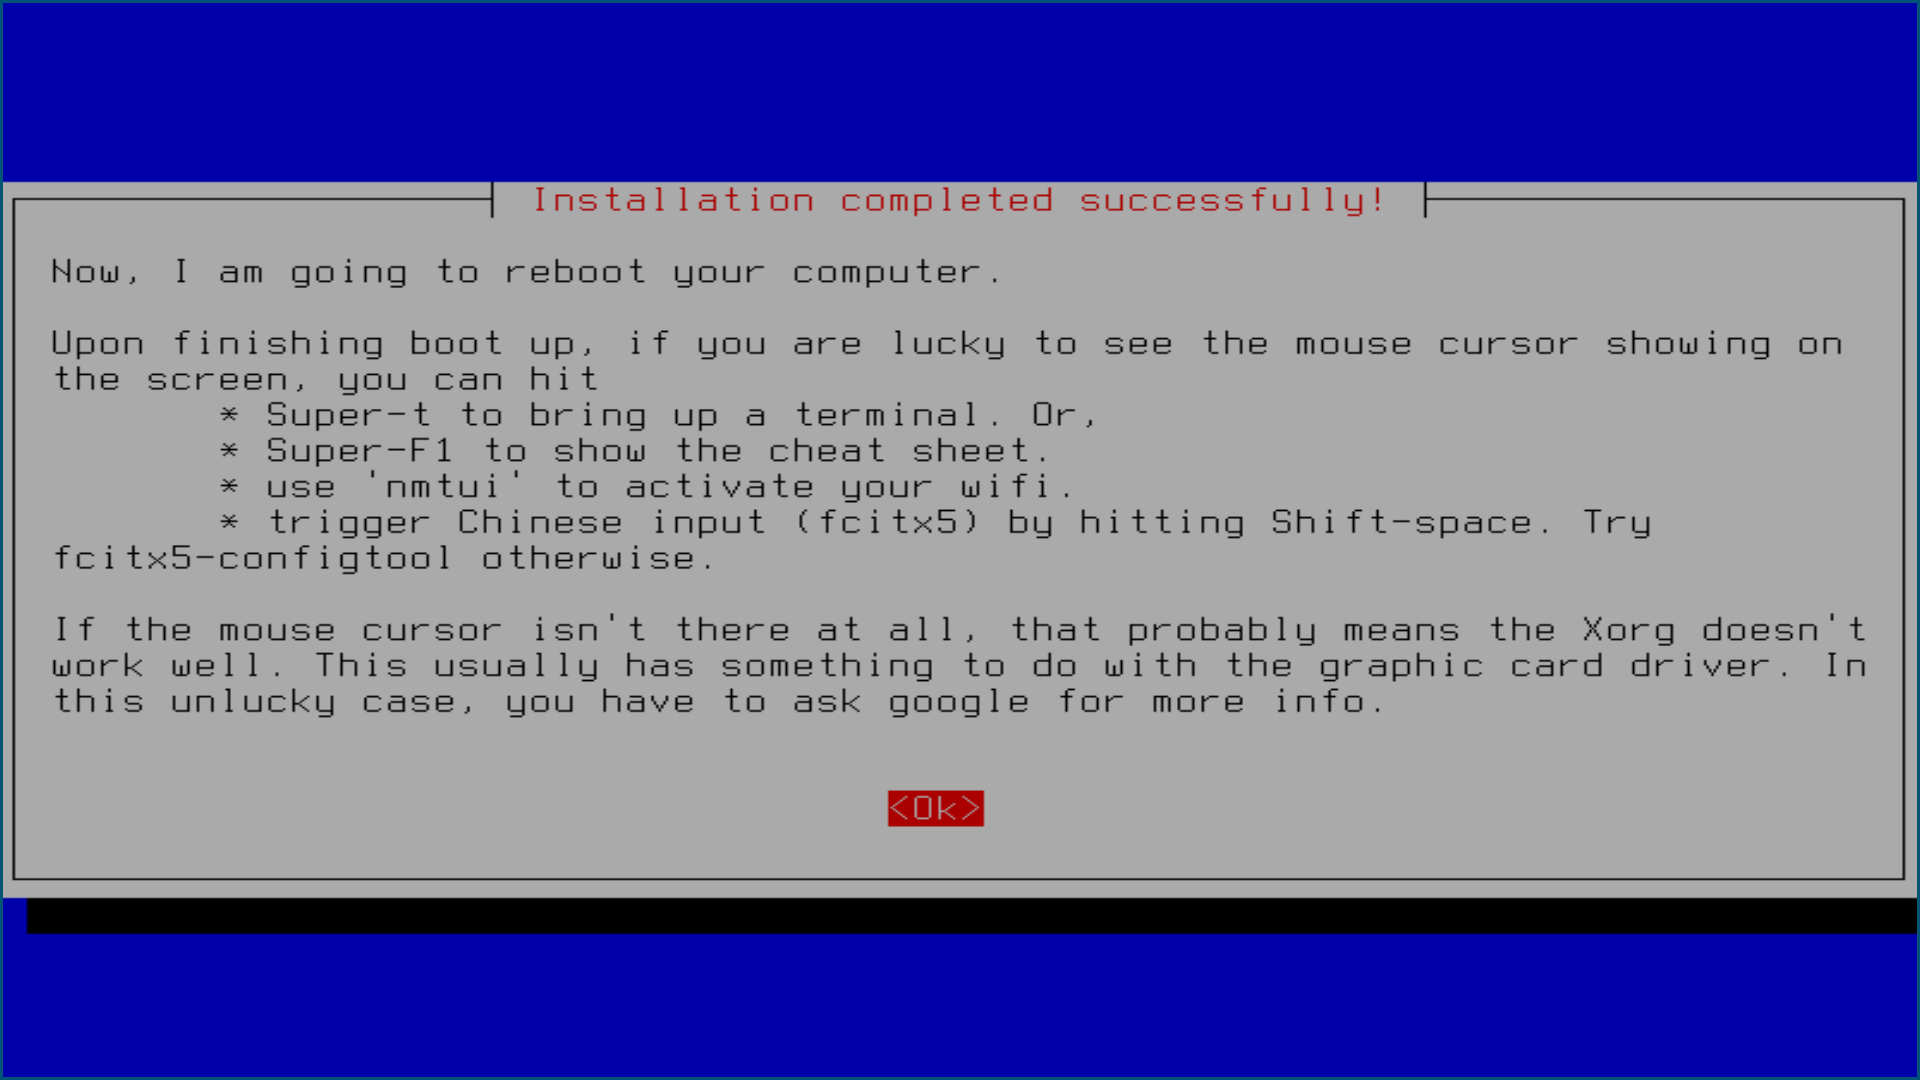
\includegraphics[width=.5\linewidth]{screenshots/46.png}
\caption{胜利结束。先仔细看看屏幕提示再回车!}
\end{figure}
\end{enumerate}
\end{enumerate}


装好之后……

\begin{enumerate}
\item 重启系统。不出意外的话,重启之后,你看到的应该就是一个终端窗口,除此之外,啥都没有,干净得令你失望。
默认的窗口管理器(Window manager)是DWM,你可以:
\begin{itemize}
\item 用 \texttt{nmtui} 来配置无线网;
\item 用 \texttt{Shift-space} 来激活中文输入法;
\item 用 \texttt{Super-q} 打开浏览器;
\item 用 \texttt{Super-l} 弹出窗口列表;
\item 用 \texttt{Super-F1} 打开“帮助墙纸”;
\item 还有很多 \texttt{Super} 开头的快捷键,自己慢慢去探索吧。
\end{itemize}
\end{enumerate}

如果重启之后,你看不到浏览器、终端、墙纸……,那么肯定是图形界面没起来,十之八九是
因为你的显卡太高级了(是Nvidia?)。你可以尝试关掉这个高级显卡,暂时使用主板上的内置显卡。
通常内置显卡要么是Intel的,要么就是AMD的,它们对Linux都很友好。具体操作如下:

\begin{enumerate}
\item 卸掉Nvidia驱动
\begin{minted}[mathescape=true,linenos=true,numbersep=5pt,frame=lines,framesep=2mm]{sh}
sudo apt purge xserver-xorg-video-{nvidia,nouveau}
\end{minted}

用 \texttt{lspci} 命令查看一下显卡的牌子。如果是Intel显卡,就安装Intel的显卡驱动:
\begin{minted}[mathescape=true,linenos=true,numbersep=5pt,frame=lines,framesep=2mm]{sh}
sudo apt install xserver-xorg-video-intel
\end{minted}

如果是AMD显卡,就安装AMD的显卡驱动:
\begin{minted}[mathescape=true,linenos=true,numbersep=5pt,frame=lines,framesep=2mm]{sh}
sudo apt install xserver-xorg-video-amdgpu
\end{minted}

如果是Radeon显卡,就安装ATI的显卡驱动:
\begin{minted}[mathescape=true,linenos=true,numbersep=5pt,frame=lines,framesep=2mm]{sh}
sudo apt install xserver-xorg-video-ati
\end{minted}

之后,重启。如果还不灵,你就自己去google吧。Have fun!
\end{enumerate}

\subsection{老办法(可以不看了)}
\label{sec:org44bac5f}
最小系统装好之后,拔出U盘,重启系统。现在我们讲讲之后的事情……
\begin{enumerate}
\item 第一件事当然是把网线插好,启动你崭新的Debian,在屏幕提示下,输入用户名、密码。
之后,你就可以通过输入命令来让电脑为你工作了。

【注意】如果你的笔记本比较新潮,比如我新买的华为Honor Magicbook,没提供有线网接口,而且
我们刚装好的最小系统里没有本机的无线网卡驱动,那么,请先参看\hyperref[sec:orgd858525]{本文末尾的附录:没有有线网卡怎么办?}
联网之后再继续。

好了,假设你解决了所有的网络问题,现在我们可以继续了……一个“最小系统”干不了多少事情,所
以我们先要安装更多的应用程序。注意,安装配置系统是管理员的工作,所以下面的很多操作自然都需要以
管理员的身份来进行,换句话说,如果你没为root设置密码的话,以后执行管理员的操作,都需要
在命令前面带上 \texttt{sudo} 。

后面的安装配置工作显然是需要联网的,所以,先检查一下你的网络状况:
\begin{verbatim}
ip a
\end{verbatim}


上面这行命令会列出你所有的网卡。仔细看一下,是否有一块网卡叫 \texttt{enpXsY} (\texttt{X} 和 \texttt{Y} 都是
数字)。仔细看看这块网卡是否已经获取到了IP地址。如果你能看到类似下面这行信息,那就没问题
了。
\begin{verbatim}
inet 192.168.1.110/24 brd 192.168.1.255 scope global dynamic eth0
\end{verbatim}

上面一行中的 \texttt{192.168.1.110} 就是有线网卡 \texttt{enp1s0} 获取到的IP地址。如果你看不到这样一
行,那么先检查一下网线是否插好了,然后敲命令:
\begin{verbatim}
sudo dhclient enpXsY
\end{verbatim}

【注释】
\begin{itemize}
\item 上面这条命令是用来获取IP地址的。没什么意外的话,你马上就可以获取到IP了。之后,再敲
\texttt{ip a} 命令确认一下。还可以 \texttt{ping} 一下,比如 \texttt{mirrors.163.com} 看看网络是否联通了。
\item \texttt{sudo} 就是要以管理员(root)的身份来执行 \texttt{dhclient enpXsY} 这条命令。前面说过,最好不要为root设置密码。当需要管理员权限时,用 \texttt{sudo} 就好。
但如果不幸你设置了root密码,那么现在你就要用 \texttt{su} 命令来变身为root
\begin{verbatim}
su
\end{verbatim}

输入密码,变成root。
\item \texttt{enpXsY} 是你的有线网卡的名字(用 \texttt{ip a} 命令可以看到)。把 \texttt{X,Y} 换成正确的数字。
\end{itemize}

【注意】如果你用的是无线网卡,那么关于联网密码设置问题,请先参看\hyperref[sec:orgf9afa95]{本文末尾的附录:无线联网时的密码设置}。

\item 修改 \texttt{sources.list} 文件
\begin{verbatim}
sudo nano /etc/apt/sources.list
\end{verbatim}

把这个文件里原有的内容全部删除掉,然后添加下面这三行:
\begin{verbatim}
deb http://mirrors.163.com/debian testing main non-free contrib
deb http://mirrors.163.com/debian testing-updates main non-free contrib
deb http://mirrors.163.com/debian testing-proposed-updates main non-free contrib
\end{verbatim}

\item 存盘退出后,刷新一下软件包列表,并更新你的最小系统:
\begin{verbatim}
sudo apt update && sudo apt dist-upgrade
\end{verbatim}


网络顺畅的话,这一步要花十几分钟的时间。
\item 现在,“机房装了什么,我就要装什么”。那就先把机房系统的软件清单弄到手,在\href{https://cs6.swfu.edu.cn/\~wx672/debian-install/list.laptop}{这里}。
这是我个人Debian笔记本电脑上的软件包列表。用 \texttt{wget} 把\href{https://gitlab.swfu.edu.cn/wx672/lecture\_notes/blob/master/linux/tutorials/install/deb-pkg-list/laptop}{这个软件清单}下载:

【注意】 \textbf{这一步不要sudo} 。
\begin{verbatim}
cd
wget -c --no-check-certificate https://cs6.swfu.edu.cn/~wx672/debian-install/01-important
\end{verbatim}


\begin{itemize}
\item 如果\url{https://cs6.swfu.edu.cn/}这个网址不好使的话,你可以试试:
\begin{itemize}
\item \url{https://github.com/wx672/lecture-notes/blob/master/linux/tutorials/install/deb-pkg-list/01-important}
\end{itemize}
\end{itemize}
\item 然后,开始大批量安装软件包:
\begin{verbatim}
sudo apt install $(cat 01-important)
\end{verbatim}


如果网络顺畅的话,这一步大概需要半个小时。通常,安装过程是不需要人为干预的。但有的软件
包在安装过程中,会停下来问你「Yes/no」。这种时候,你最好耐心把屏幕提示看明白。一般来讲,
直接按「回车」就好。
\item 一切顺利的话,网卡、声卡、显卡……都不需要额外的操心。但如果运气不太好的话(这通常是人品
问题,因为你以学习的名义向家里要钱,最终却为了玩游戏而买了个声卡、显卡都特新潮的游戏机),
那么……假设你幡然悔悟了,可以看看本文末尾的附录:\hyperref[sec:org81b3258]{关于硬件配置}。
\item 如果像我一样,你也是\hyperref[sec:orgf9afa95]{用USB无线网卡完成的安装},那么现在你应该可以拔掉USB无线网卡了。同时
把刚才添加进 \texttt{/etc/network/interfaces} 文件的四行删除,或者注释掉。重启系统之后,用
\texttt{nmtui} 来连接无线网:
\begin{verbatim}
nmtui
\end{verbatim}

这是个界面挺友好的小工具,不用人教,你就会用。
\item 上面安装的 \texttt{01-important} 文件中的软件包都是我认为必不可少的,但并不充分。如果要满足日
常需求,我觉得你最好把下面这些包也装上。
\begin{itemize}
\item \url{https://cs6.swfu.edu.cn/\~wx672/debian-install/02-recommend}
\item \url{https://cs6.swfu.edu.cn/\~wx672/debian-install/03-chinese}
\end{itemize}

我日常使用的大概就是这些了。
\end{enumerate}

\section{配置(可以不看了)}
\label{sec:orge8febae}

\subsection{sudo 的时候总要问密码,是不是很烦?}
\label{sec:org5e59d5a}
那就不让它问了:
\begin{enumerate}
\item 建立一个新文件
\begin{verbatim}
sudo nano /etc/sudoers.d/your-user-name
\end{verbatim}

【注意】把 \texttt{your-user-name} 改成你自己的用户名。

\item 在里面写这么一行:
\begin{verbatim}
your-user-name  ALL = NOPASSWD: ALL
\end{verbatim}

【注意】把 \texttt{your-user-name} 改成你自己的用户名。
\item 改一下权限:
\begin{verbatim}
sudo chmod 0440 /etc/sudoers.d/your-user-name
\end{verbatim}

这以后 \texttt{sudo} 就不再问密码了。

\item 如果前面你不是用 \texttt{sudo} ,而是用 \texttt{su} 获得root权限的,那么现在应该退回到普通用户身份:
\begin{verbatim}
exit
\end{verbatim}

总之,命令行提示符不是 \texttt{\#}, 而是 \texttt{\$}, 就对了。
\end{enumerate}

\subsection{dotfile}
\label{sec:org90f7f21}
现在你的系统和机房的差不多一样了,唯一的差别就是你还没配置呢。
配置是个琐碎的事情,比较省事的办法就是把我的配置文件拷贝过来。最省事的拷贝方式就是
git( \textbf{以普通用户的身份来做} ):
\begin{minted}[mathescape=true,linenos=true,numbersep=5pt,frame=lines,framesep=2mm]{sh}
cd
git clone https://github.com/wx672/dotfile.git
#或者
git clone https://cs6.swfu.edu.cn/~wx672/dotfile/.git
\end{minted}

上面两个网址应该都可以。 \texttt{git} 是著名的源代码管理工具,也就是版本控制工具。用它来管理配置文
件也非常顺手。上面的命令完成之后, \texttt{ls} 一下,应该可以看到,你的 \texttt{\$HOME} 目录里多了一个子
目录 \texttt{dotfile} ,里面放的都是杂七杂八的配置文件。

现在把 \texttt{dotfile} 目录里所有以 \texttt{dot.} 开头的文件和目录都链接到 \texttt{\$HOME} 目录里,
\begin{enumerate}
\item 先确保你在 \texttt{\$HOME}:
\begin{verbatim}
cd
\end{verbatim}

\item 把旧的 \texttt{.bash*} 文件都删掉:
\begin{verbatim}
rm -f .bash*
\end{verbatim}

\item 做链接:
\begin{verbatim}
ln -sf dotfile/dot.* .
ln -sf dotfile/help/dot.* .
\end{verbatim}


现在 \texttt{ls} 一下,你会发现 \texttt{\$HOME} 目录里有了很多 \texttt{dot.} 开头的文件。

\item 把所有的 \texttt{dot.} 都变成 \texttt{.}, 也就是把文件名前面的 \texttt{dot} 都去掉,只留下 \texttt{.}:
\begin{verbatim}
rename 's/dot//' dot.*
\end{verbatim}

现在用 \texttt{ls -al} 检查一下,我们需要的配置文件(也就是‘点’开头的文件)应该都在 \texttt{\$HOME} 目录里了。

\item 我的Emacs配置里用到了很多插件,自然你也需要它们,否则Emacs不能正常工作。
\begin{enumerate}
\item 先把我的插件包下载下来
\begin{minted}[mathescape=true,linenos=true,numbersep=5pt,frame=lines,framesep=2mm]{sh}
wget -c --no-check-certificate http://cs6.swfu.edu.cn/~wx672/debian-install/elpa.tgz
\end{minted}
\item 放到Emacs的配置文件目录里
\begin{minted}[mathescape=true,linenos=true,numbersep=5pt,frame=lines,framesep=2mm]{sh}
mv elpa.tgz ~/.emacs.d/
\end{minted}
\item 然后解压缩
\begin{minted}[mathescape=true,linenos=true,numbersep=5pt,frame=lines,framesep=2mm]{sh}
cd ~/.emacs.d
tar zxf elpa.tgz
\end{minted}
\item 测试一下
\begin{minted}[mathescape=true,linenos=true,numbersep=5pt,frame=lines,framesep=2mm]{sh}
emacs --debug-init
\end{minted}
如果报错,就把出错信息发给我(wx672ster@gmail.com)。  
当然,如果你能自己解决问题那再好不过了。
\end{enumerate}
\end{enumerate}

\subsection{Auto login}
\label{sec:orgb7c3a20}
简单起见,我们只讲“怎么做”,先不管“为什么”。
\begin{enumerate}
\item 拷贝配置文件
\begin{minted}[mathescape=true,linenos=true,numbersep=5pt,frame=lines,framesep=2mm]{sh}
sudo cp -r ~/dotfile/etc/systemd/system/getty@tty1.service.d/ /etc/systemd/system/
\end{minted}
注意, \texttt{\textasciitilde{}} (也就是波浪线), 它代表你的 \texttt{\$HOME} 目录。
\item 修改
\begin{minted}[mathescape=true,linenos=true,numbersep=5pt,frame=lines,framesep=2mm]{sh}
sudo nano /etc/systemd/system/getty@tty1.service.d/override.conf
\end{minted}
在这个 \texttt{override.conf} 文件里应该只有如下三行:
\begin{verbatim}
[Service]
ExecStart=
ExecStart=-/sbin/agetty --autologin wx672 --noclear %I $TERM
\end{verbatim}
你只要把其中的 \texttt{wx672} 改成你自己的用户名就可以了。
\end{enumerate}

\subsection{中文语言环境}
\label{sec:org41cfbcf}
注意,我们其实并不需要一套纯正的中文环境,我们只是需要输入和阅读中文。
其它方面,比如窗口菜单、提示信息、man page,我觉得还是看英文比较好。

千万别说“我英文差,还是用中文算了”。要知道,就是因为你
“这个差、那个不行、这个不懂、那个不会……”所以你才来上学的,不是吗?
既然知道“差”,那就该好好学习,提高它。
英文是用熟的,如果你总是回避它,就总也不会长进了。

好了,下面我们来配置一个简单的中文环境。相关中文字体我们已经安装好了。下面只需要:
\begin{enumerate}
\item 安装中文字体和输入法。
\begin{minted}[mathescape=true,linenos=true,numbersep=5pt,frame=lines,framesep=2mm]{sh}
cd
wget -c --no-check-certificate https://cs6.swfu.edu.cn/~wx672/debian-install/03-chinese
sudo apt install `cat 03-chinese`
\end{minted}

\item 选择 \texttt{locale}
\begin{minted}[mathescape=true,linenos=true,numbersep=5pt,frame=lines,framesep=2mm]{sh}
sudo dpkg-reconfigure locales
\end{minted}
在这一长串列表中,只要选中
\begin{itemize}
\item[{$\boxtimes$}] \texttt{en\_US.UTF-8 UTF-8}
\item[{$\boxtimes$}] \texttt{zh\_CN.GB18030 GB18030}
\item[{$\boxtimes$}] \texttt{zh\_CN.UTF-8 UTF-8}
\end{itemize}
就可以了。默认语言环境选 \texttt{None} 。

\item 拷贝一个小配置文件:
\begin{minted}[mathescape=true,linenos=true,numbersep=5pt,frame=lines,framesep=2mm]{sh}
sudo cp ~/dotfile/etc/default/locale /etc/default
\end{minted}

\item 顺带再拷贝一个小文件:
\begin{minted}[mathescape=true,linenos=true,numbersep=5pt,frame=lines,framesep=2mm]{sh}
sudo cp ~/dotfile/etc/default/keyboard /etc/default
\end{minted}
这是把你的 \texttt{CapsLock} 键变成 \texttt{Ctrl} 键,
因为Unix用户经常要用 \texttt{Ctrl} 键,从来不用 \texttt{CapsLock} 。

好了,现在安装配置的工作基本就结束了。你可以重启一下系统。
系统重启后,看到的应该就是学院机房里那个没有桌面的“桌面系统”了。
不记得快捷键了?按 \texttt{Super-F1} 。

中文输入法,我选用的是 \texttt{fcitx}, 因为感觉它的bug要少一些,比较稳定。
如果你需要配置它的话,就:
\begin{minted}[mathescape=true,linenos=true,numbersep=5pt,frame=lines,framesep=2mm]{sh}
fcitx-configtool
\end{minted}
你最好和我一样,用 \texttt{Shift-space} 来激活输入法,因为 \texttt{Ctrl-space} 在Emacs里有特殊用途。

注意:fcitx依赖于dbus-x11,而显然fcitx软件包的维护者忽略了这个小细节。那么我们就自己把
它装上呗:
\begin{minted}[mathescape=true,linenos=true,numbersep=5pt,frame=lines,framesep=2mm]{sh}
sudo apt install dbus-x11
\end{minted}
\end{enumerate}

\section{附录:没有有线网卡怎么办?}
\label{sec:orgd858525}
办法很多:
\begin{enumerate}
\item 用Android手机的USB Tethering功能。以我自己的手机系统为例(LineageOS 16.0/Android 9),
很简单,
\begin{enumerate}
\item 用USB线连接手机和电脑;
\item 在手机的「系统设置」里有个搜索框,在里面输入“tethering”,马上就能找到“Hotspot \&
Tethering”,激活里面的USB Tethering功能就行了;
\item 在电脑上,敲命令 \texttt{ip a} 应该能看到一块有线网卡。比如,
\begin{verbatim}
3: enp2s0f4u2: <BROADCAST,MULTICAST,UP,LOWER_UP> mtu 1500 qdisc pfifo_fast state UNKNOWN group default qlen 1000
   link/ether 26:b1:c7:c5:02:1f brd ff:ff:ff:ff:ff:ff
\end{verbatim}
从上面的屏幕输出信息可以看到,这块有线网卡的名字是 \texttt{enp2s0f4u2} 。然后,以root身份,
敲下面这条命令:
\begin{minted}[mathescape=true,linenos=true,numbersep=5pt,frame=lines,framesep=2mm]{sh}
sudo dhclient enp2s0f4u2
\end{minted}
你就可以获得一个IP地址了,也就是说,你已经成功联网了。
\end{enumerate}
\item 去找一个USB无线网卡试试。我找到一个Realtek的指甲盖大小的USB无线网卡,不需要驱动,插上就
能用。我也尝试过两个比较古老的tp-link无线网卡,不好使。
\item 另外,如果你真的和我一样,用的是华为Honor Magicbook,那么也许你不必去找USB网卡,可以先
试试能否让内置网卡工作。Magicbook的内置网卡是Intel的。既然完成后面的安装步骤之后它能正
常工作,那我想,现在使使劲应该也能解决问题吧。但毕竟我还没有亲自尝试过,所以只能先给出
一些想法:
\begin{itemize}
\item 之所以内置网卡暂时不工作,我怀疑是我们用来安装最小系统的iso文件不够新。它是以Debian稳
定版(stretch)为基础做出来的,其中的内核(4.9)和相应固件(firmware-iwlwifi)都偏旧,
可能尚不支持这么新潮(2018年)的硬件。所以,可以试试把内核和相应固件从稳定版更新到测
试版(buster)。在没有网络连接的情况下,显然这需要我们另找办法下载,并手动安装一些软
件包,包括:
\begin{itemize}
\item \href{https://packages.debian.org/buster/linux-image-amd64}{linux-image-amd64}
\item \href{https://packages.debian.org/buster/firmware-iwlwifi}{firmware-iwlwifi}
\item 还有若干被上述两个软件包依赖的软件包
\end{itemize}
\item 一些参考链接:
\begin{itemize}
\item \href{https://unix.stackexchange.com/questions/283722/how-to-connect-to-wifi-from-command-line}{How to connect to WiFi from command line?}
\item \href{https://askubuntu.com/questions/974/how-can-i-install-software-or-packages-without-internet-offline}{How can I install software packages without Internet?}
\item \href{https://commandlinefanatic.com/cgi-bin/showarticle.cgi?article=art016}{Installing Debian without a Network}
\item \href{https://wiki.debian.org/WiFi}{Debian Wiki --- WiFi}
\end{itemize}
\end{itemize}
\item 如果上述办法都不成功,那么这招肯定行,就是笨点。直接去下面这些镜像站下载完整的安装盘。
\begin{itemize}
\item \url{http://mirrors.163.com/debian-cd/current/amd64/iso-dvd/}
\item \url{http://mirrors.ustc.edu.cn/debian-cd/current/amd64/iso-dvd/}
\end{itemize}

完整的DVD安装盘包含3个iso文件,你可以先下载第一个试试。如果里面有了你需要的无线网卡驱动
和相关程序,那么激活网卡之后,你就可以直接网络安装了,无需下载其它的iso文件了。
\end{enumerate}

\subsection{无线联网时的密码设置}
\label{sec:orgf9afa95}
无线联网时通常是要输入密码的,所以我们需要修改一个配置文件 \texttt{/etc/network/interfaces} ,很
简单,编辑这个小文件:
\begin{minted}[mathescape=true,linenos=true,numbersep=5pt,frame=lines,framesep=2mm]{sh}
sudo nano /etc/network/interfaces
\end{minted}
\texttt{nano} 是个很简单的编辑器,用起来应该不会有什么困难吧。 
\texttt{nano} 窗口的最下两行都是快捷键提示,最重要的两个是:
\begin{enumerate}
\item 存盘: \texttt{Ctrl-o}
\item 退出: \texttt{Ctrl-x}
\end{enumerate}

在这个文件的最后加上如下几行:
\begin{verbatim}
iface tmp inet dhcp
wireless-essid MY-ESSID
wpa-ssid MY-ESSID
wpa-psk PASSWORD
\end{verbatim}
【注意】把 \texttt{MY-ESSID} 和 \texttt{PASSWORD} 换成你自己的无线网络的名字和密码。

然后,用下面这条命令来连接无线网:
\begin{minted}[mathescape=true,linenos=true,numbersep=5pt,frame=lines,framesep=2mm]{sh}
sudo ifup WLANCARD=tmp
\end{minted}
【注意】把 \texttt{WLANCARD} 换成你自己的无线网卡的名字,网卡的名字通常是w开头的,比如我的无线
网卡名字就是 \texttt{wlp1s0} ,那么我用的联网命令就是:
\begin{minted}[mathescape=true,linenos=true,numbersep=5pt,frame=lines,framesep=2mm]{sh}
sudo ifup wlp1s0=tmp
\end{minted}

\section{附录:关于硬件配置}
\label{sec:org81b3258}
首先,当然是要搞清楚你到底有哪些硬件。很简单:
\begin{minted}[mathescape=true,linenos=true,numbersep=5pt,frame=lines,framesep=2mm]{sh}
lspci
#想看更详细的信息,就:
lspci -vvv
\end{minted}

总之, \texttt{lspci} 能列出你所有外围设备的详细信息。然后,如果
你的有线或无线网卡是Realtek,或者Atheros牌子的,那么你需要安装相应的firmware(固件)。
\begin{minted}[mathescape=true,linenos=true,numbersep=5pt,frame=lines,framesep=2mm]{sh}
#如果是Realtek网卡,就:
sudo apt install firmware-realtek
#如果是Atheros网卡,就:
sudo apt install firmware-atheros
#如果是Intel网卡,就:
sudo apt install firmware-iwlwifi
\end{minted}

并不是所有的网卡都需要安装相应的固件,甚至上面提到的Realtek, Atheros, Intel网卡,即使不
装固件,网卡也可能工作,但未必那么稳定。所以,既然有固件,那还是装上比较
好。同样,针对声卡、显卡,Debian库里也有很多固件。下面这条命令可以列出库里所有的固件包:
\begin{minted}[mathescape=true,linenos=true,numbersep=5pt,frame=lines,framesep=2mm]{sh}
aptitude search ^firmware
\end{minted}
大概也就三十几个吧。找找有没有和你的硬件相关的。怎么知道是否相关呢?看看固件包的详细信
息呗,比如:
\begin{minted}[mathescape=true,linenos=true,numbersep=5pt,frame=lines,framesep=2mm]{sh}
apt show firmware-atheros
\end{minted}
于是就知道了这个固件适用于哪些网卡。

关于显卡,听说Nvidia显卡比较难伺候,好在我从来没碰到过,因为只有游戏本才配置这么贵的显
卡。如果你(曾经人品不好)不幸碰到了,那么,省事起见,我建议你暂时不要用它,就用主板上内置
的(通常是Intel)显卡就好。直到有一天你成了一个熟练的Linux用户之后,再把它激活。
\section{附录:\LaTeX{} (非必须)}
\label{sec:orgb7905fe}
在Linux平台,你不用非要学习使用\LaTeX{}来排版你的文章、报告、论文,
因为你已经有了一套开源的office软件。如果前面的事情你都顺利完成了,那么现在只需要按
\texttt{Super-o} (键盘上那个Win键,我们叫它Super键)
就可以调出著名的Libreoffice了。然后,你完全可以像在Windows平台上那样写东西。

但是,「你们这些使用Linux的人,不就是“装逼、扮酷”嘛」,既然他嫌你酷,那么你就再酷一点嘛。
TeXLive是一套优秀而庞大的排版系统,我们只需要安装使用它提供的少数十几个软件包就够了。

我个人用到的\LaTeX{}软件包列表在\href{https://cs6.swfu.edu.cn/\~wx672/debian-install/list.texlive}{这里}:
\begin{verbatim}
$ wget -c --no-check-certificate http://cs6.swfu.edu.cn/~wx672/debian-install/04-texlive
$ sudo apt install `cat 04-texlive`
\end{verbatim}

上面这两行命令和我们前面用到的很相似吧。第一行是下载 \texttt{04-texlive} 文件,
也就是我的TeXLive软件包列表。第二行是安装文件里的所有软件包。
安装好以后,如果想“酷”,那么你要做如下几件事情:
\begin{enumerate}
\item 熟悉Emacs的使用。为什么非要用Emacs啊?因为它为编辑\LaTeX{}文件提供了最好的支持。而且,我不
想在这里唠唠叨叨,如果你想看我为Emacs做的广告,可以看我在「知乎」上写的一个小答案:
\begin{itemize}
\item \url{https://www.zhihu.com/question/30955165/answer/70799403}
\end{itemize}

顺带贩卖一下我为Debian做的广告:
\begin{itemize}
\item \url{https://www.zhihu.com/question/19676224/answer/29321011}
\end{itemize}

\item 学习一点关于\LaTeX{}的基础知识,我觉得两三个小时应该够了吧。我推荐 \texttt{lshort}:
\begin{verbatim}
texdoc -l lshort
\end{verbatim}

上面这条命令会列出几个相关的PDF文件,你要关注的是前两个:
\begin{verbatim}
1 /usr/share/texlive/texmf-dist/doc/latex/lshort-english/lshort.pdf
2 /usr/share/texlive/texmf-dist/doc/latex/lshort-chinese/lshort-zh-cn.pdf
\end{verbatim}

我鼓励你看英文原版,至少应该中英对照着看吧。
\item 如果你打算尝试用\LaTeX{}来写你的毕业论文,那么我为你提供了点小帮助:
\begin{itemize}
\item \url{https://github.com/wx672/texmf/tree/master/doc/latex/swfu/swfuthesis}
\item \url{https://cs6.swfu.edu.cn/\~wx672/texmf/doc/latex/swfu/swfuthesis/}
\end{itemize}
上面两个链接里的内容是一样的,看哪个都行。有问题可以向我求助。

Happy LaTeXing!
\end{enumerate}
\end{document}
%%% Local Variables:
%%% mode: latex
%%% TeX-master: t
%%% End:
